\begin{frame}{$\tAmp_{2B}^{\mathrm{Re}}$ at $P_L=-1$: lattice coordinates}
\centering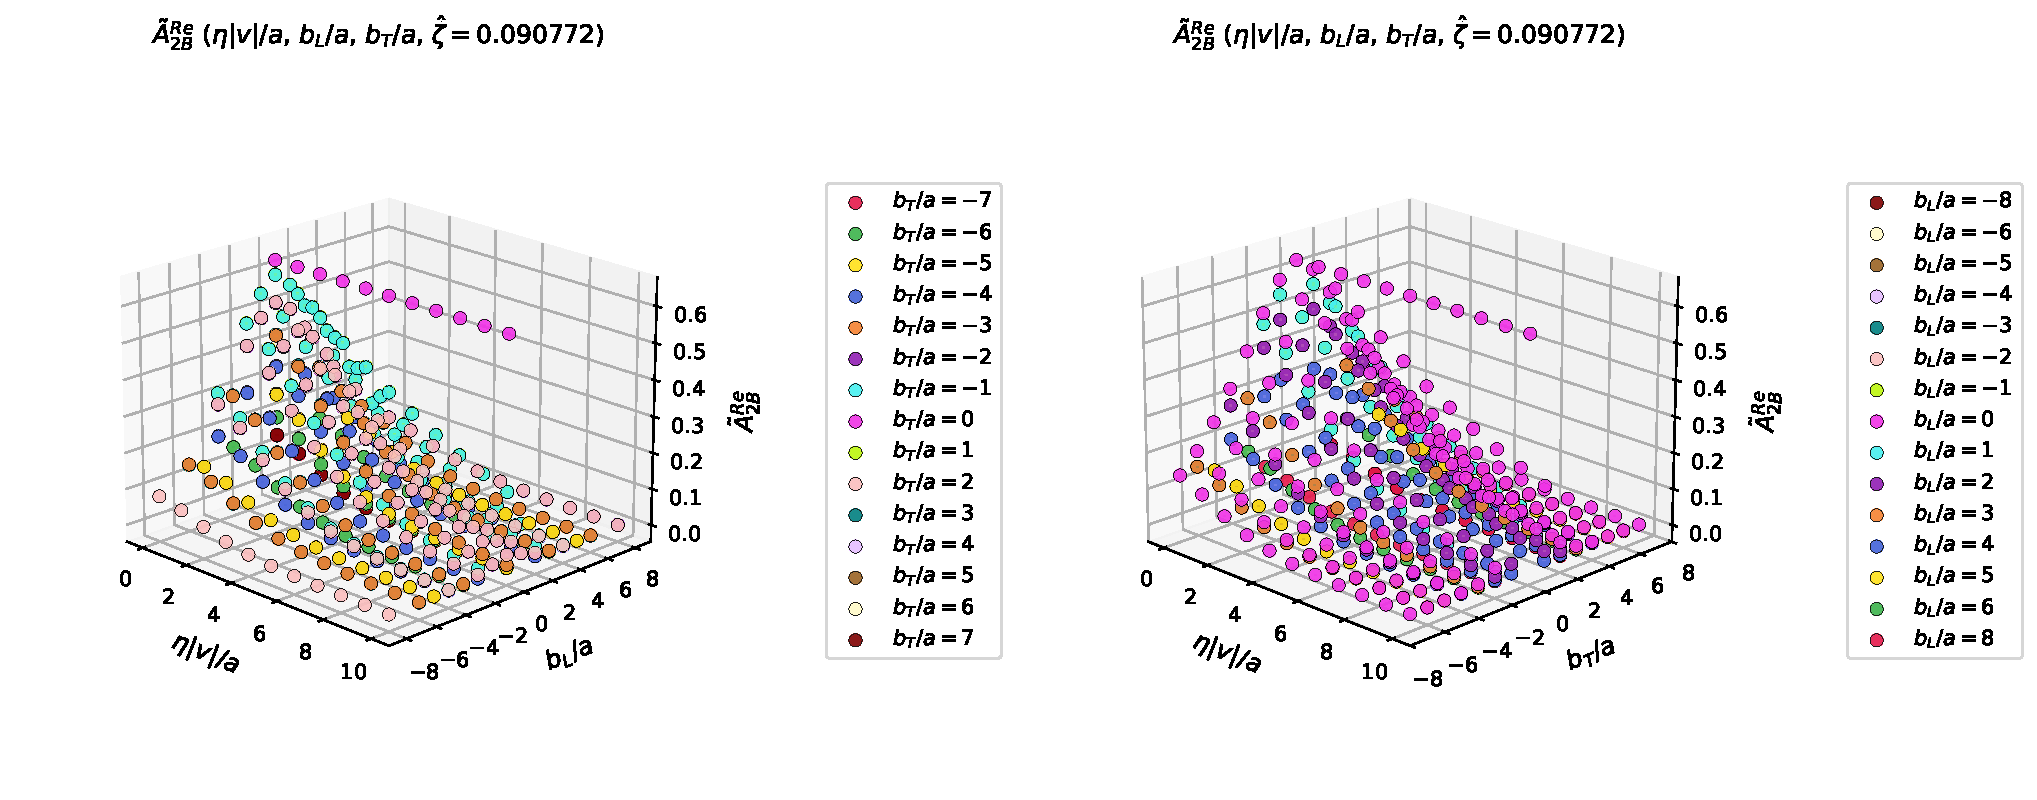
\includegraphics[width=0.98\linewidth,height=0.73\textheight,keepaspectratio]{ReA2B_PL-1_3D.pdf}\\[1mm]
{\small $\zetahat=0.090772$; $(b_L,b_T)$; staple-length dependence}
\figsrc{Thesis, Ch. 5: raw amplitude profiles; complete original panels.}
\end{frame}

\begin{frame}{$\tAmp_{2B}^{\mathrm{Re}}$ at $P_L=-1$: invariant coordinates}
\centering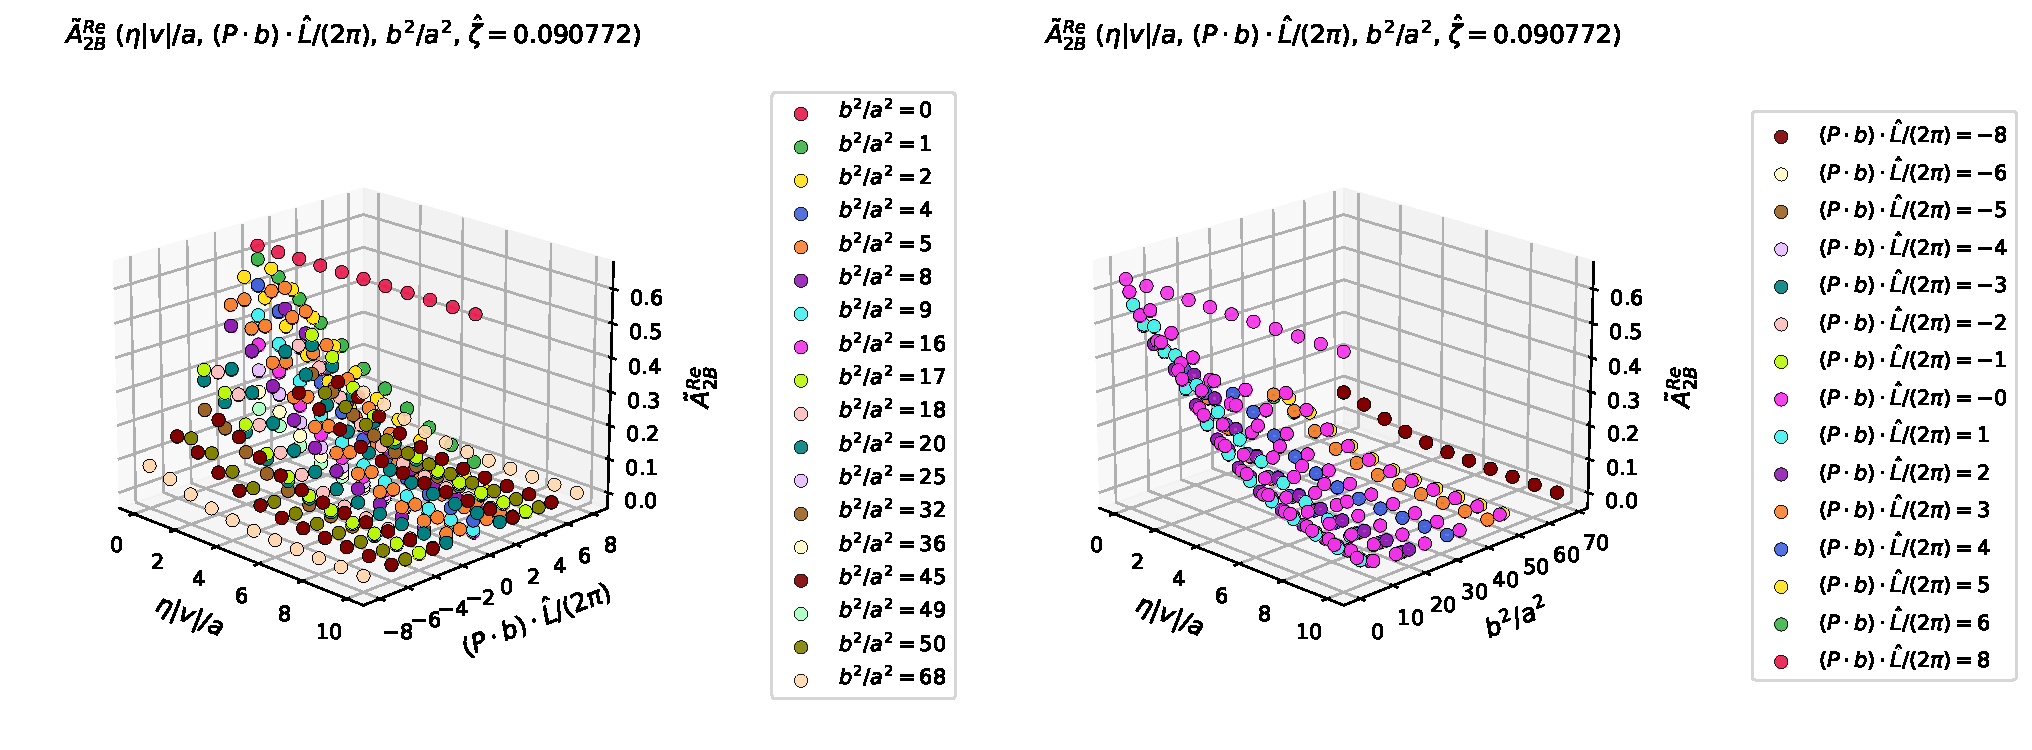
\includegraphics[width=0.98\linewidth,height=0.73\textheight,keepaspectratio]{ReA2B_Pb_bsq_PL-1_3D.pdf}\\[1mm]
{\small $\zetahat=0.090772$; $(\nu,s)$; staple-length dependence}
\figsrc{Thesis, Ch. 5: raw amplitude profiles; complete original panels.}
\end{frame}

\begin{frame}{$\tAmp_{2B}^{\mathrm{Im}}$ at $P_L=-1$: lattice coordinates}
\centering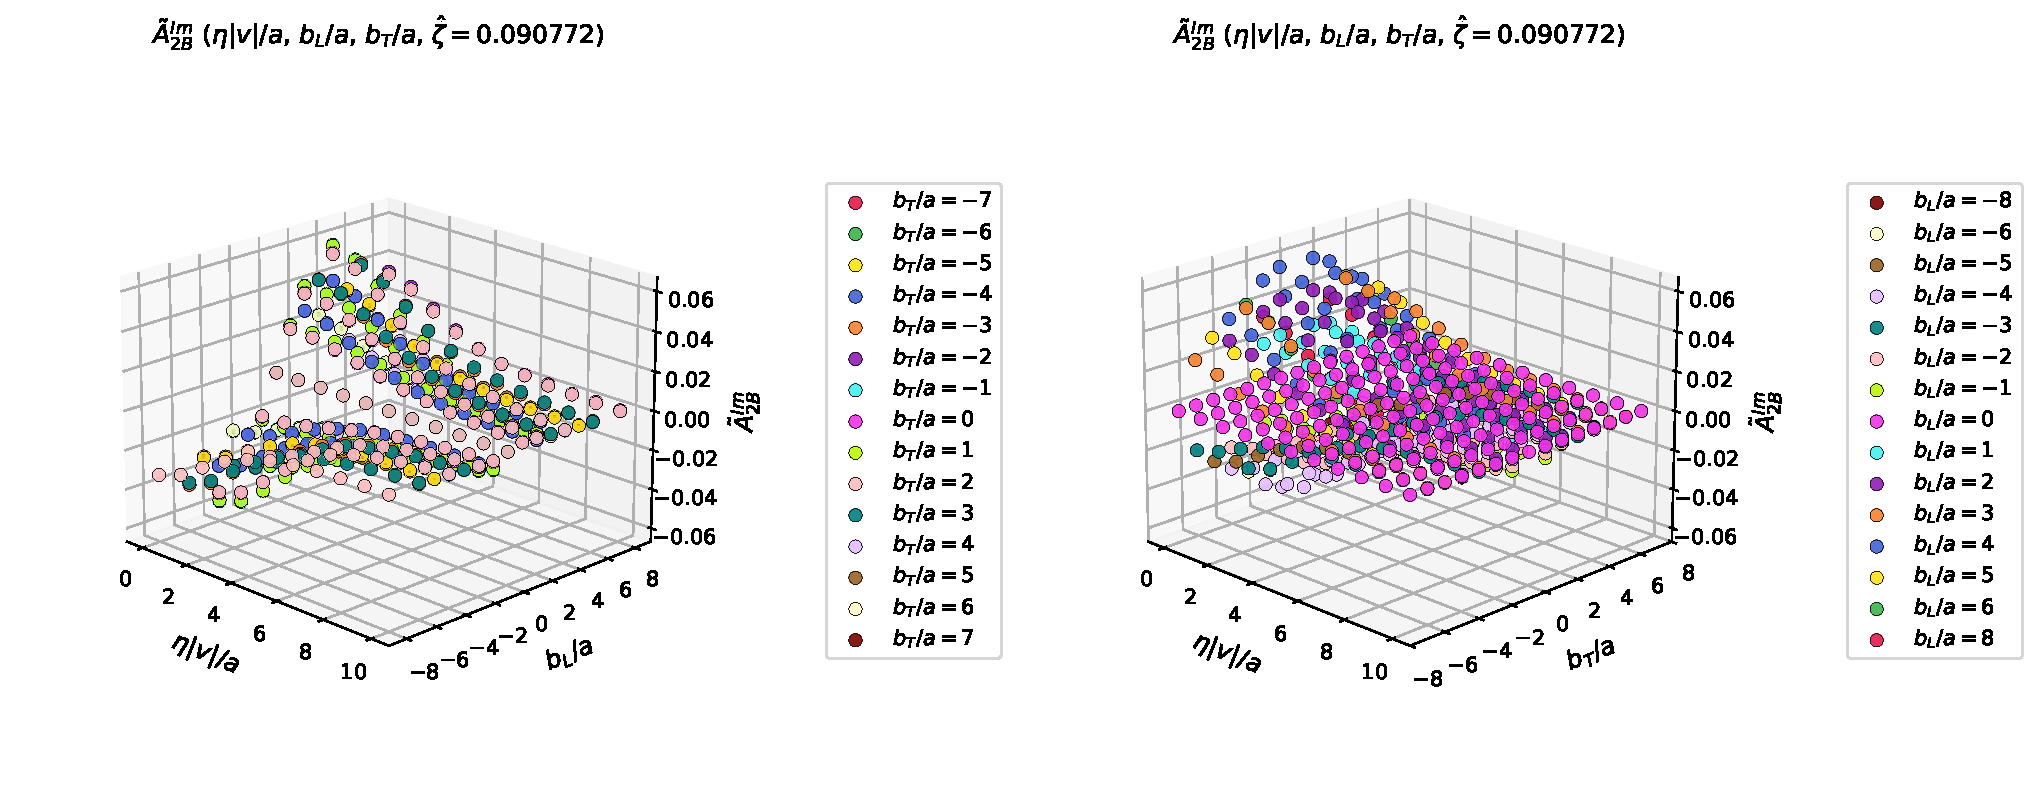
\includegraphics[width=0.98\linewidth,height=0.73\textheight,keepaspectratio]{ImA2B_PL-1_3D.pdf}\\[1mm]
{\small $\zetahat=0.090772$; $(b_L,b_T)$; staple-length dependence}
\figsrc{Thesis, Ch. 5: raw amplitude profiles; complete original panels.}
\end{frame}

\begin{frame}{$\tAmp_{2B}^{\mathrm{Im}}$ at $P_L=-1$: invariant coordinates}
\centering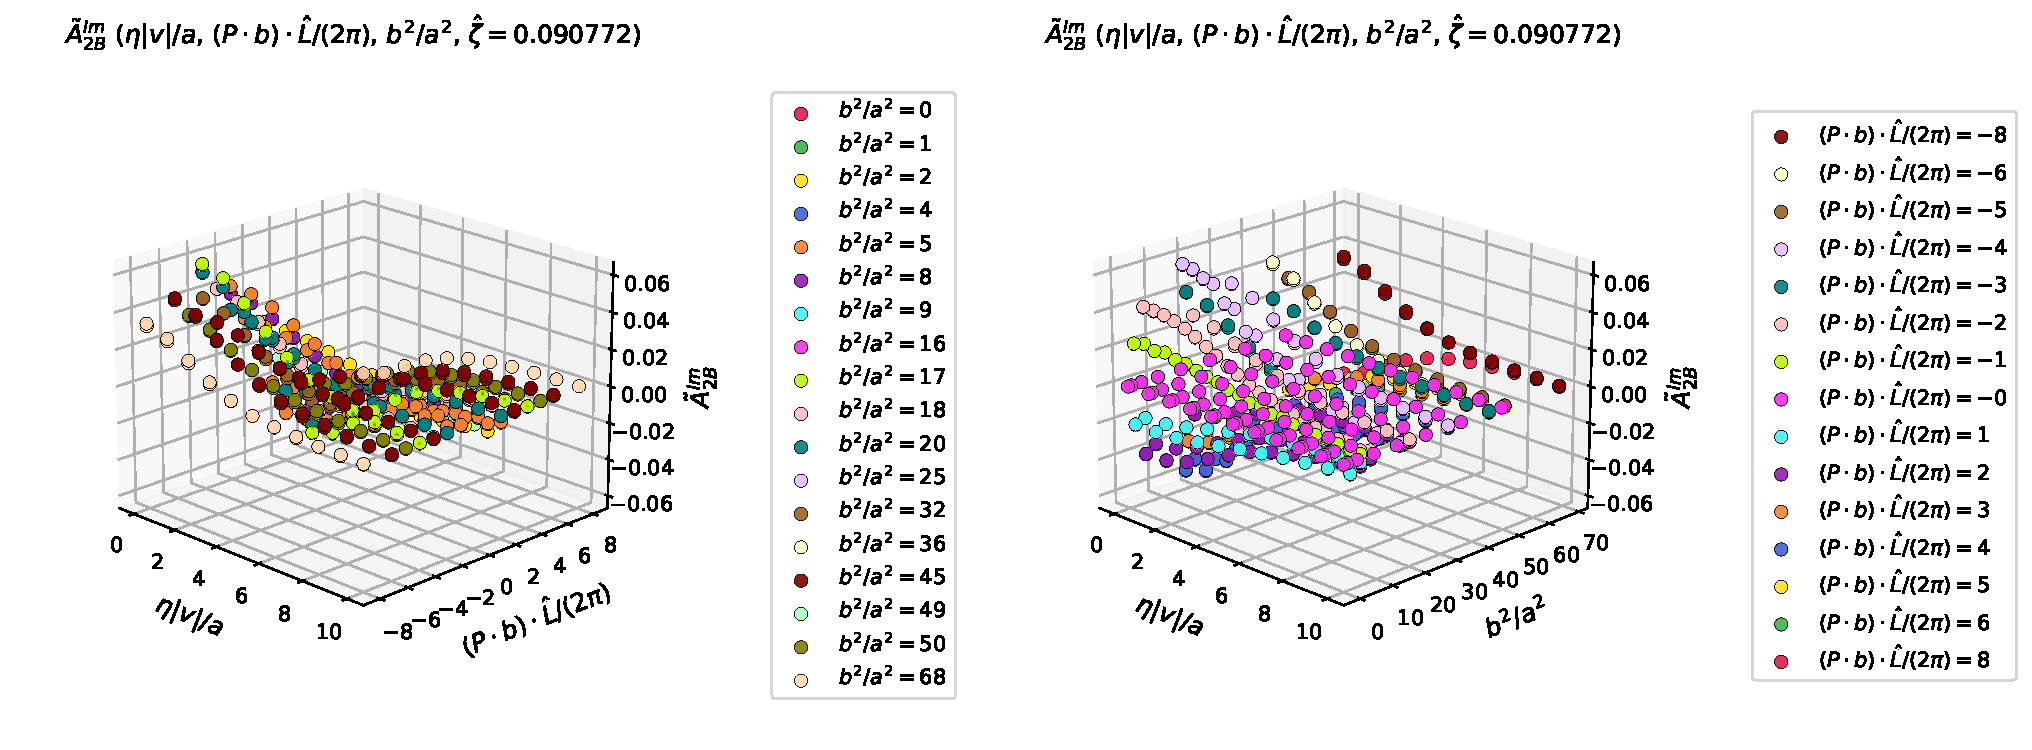
\includegraphics[width=0.98\linewidth,height=0.73\textheight,keepaspectratio]{ImA2B_Pb_bsq_PL-1_3D.pdf}\\[1mm]
{\small $\zetahat=0.090772$; $(\nu,s)$; staple-length dependence}
\figsrc{Thesis, Ch. 5: raw amplitude profiles; complete original panels.}
\end{frame}

\begin{frame}{$\tAmp_{12B}^{\mathrm{Re}}$ at $P_L=-1$: lattice coordinates}
\centering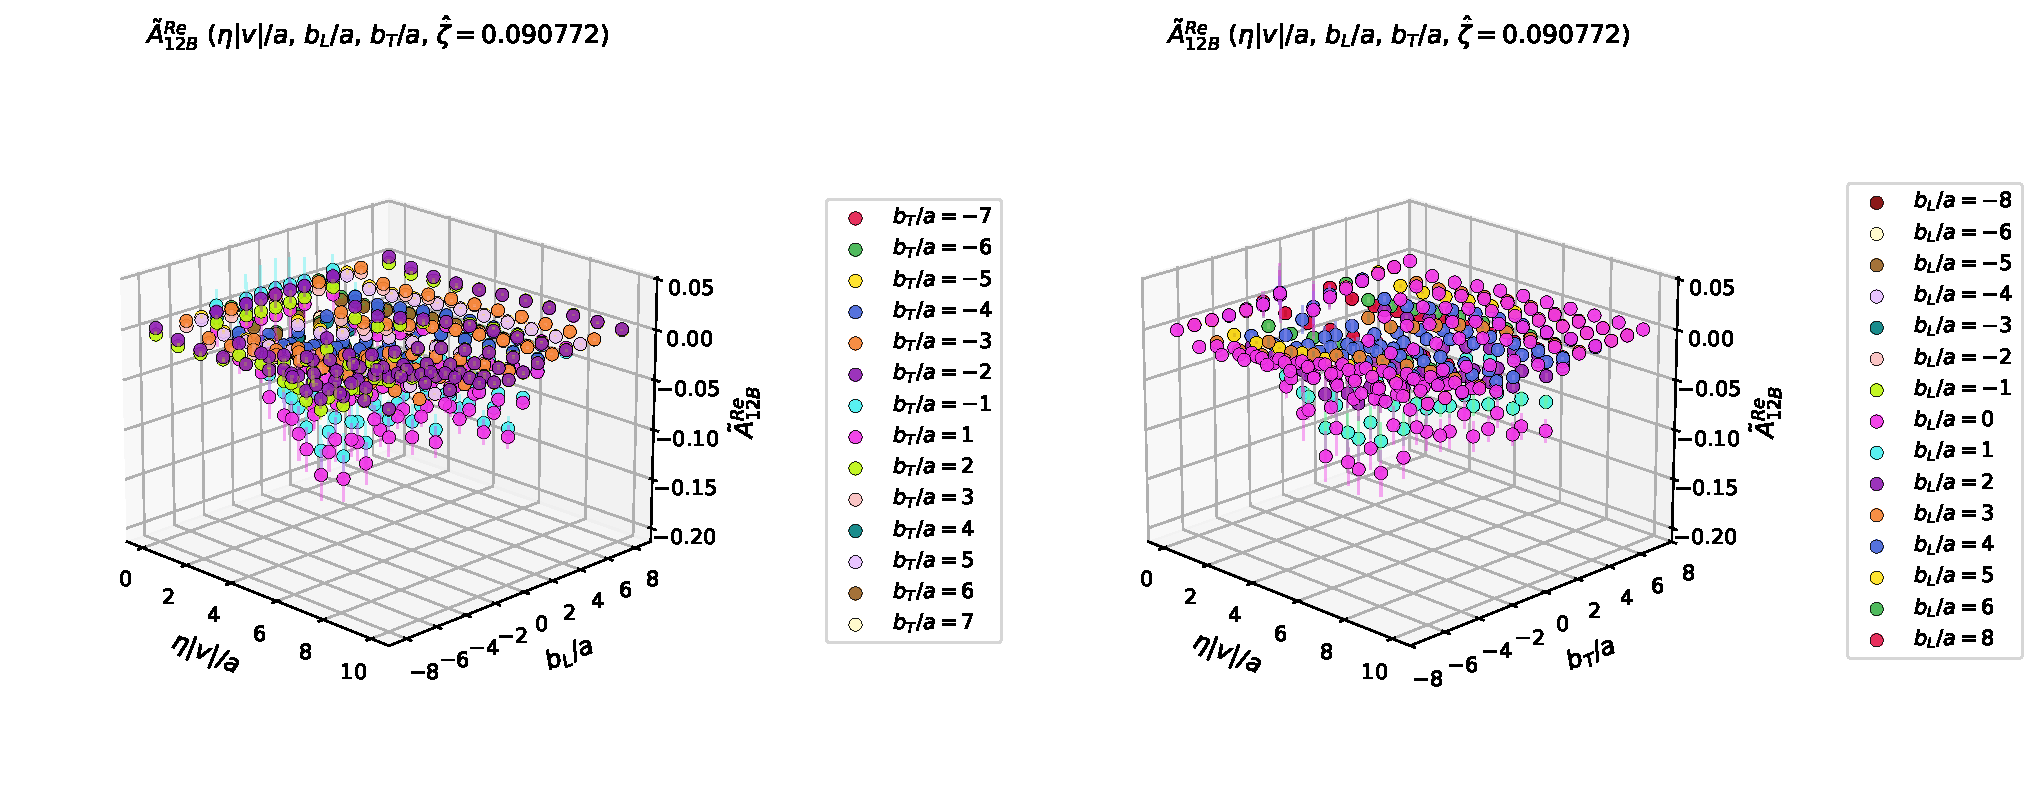
\includegraphics[width=0.98\linewidth,height=0.73\textheight,keepaspectratio]{ReA12B_PL-1_3D.pdf}\\[1mm]
{\small $\zetahat=0.090772$; $(b_L,b_T)$; staple-length dependence}
\figsrc{Thesis, Ch. 5: raw amplitude profiles; complete original panels.}
\end{frame}

\begin{frame}{$\tAmp_{12B}^{\mathrm{Re}}$ at $P_L=-1$: invariant coordinates}
\centering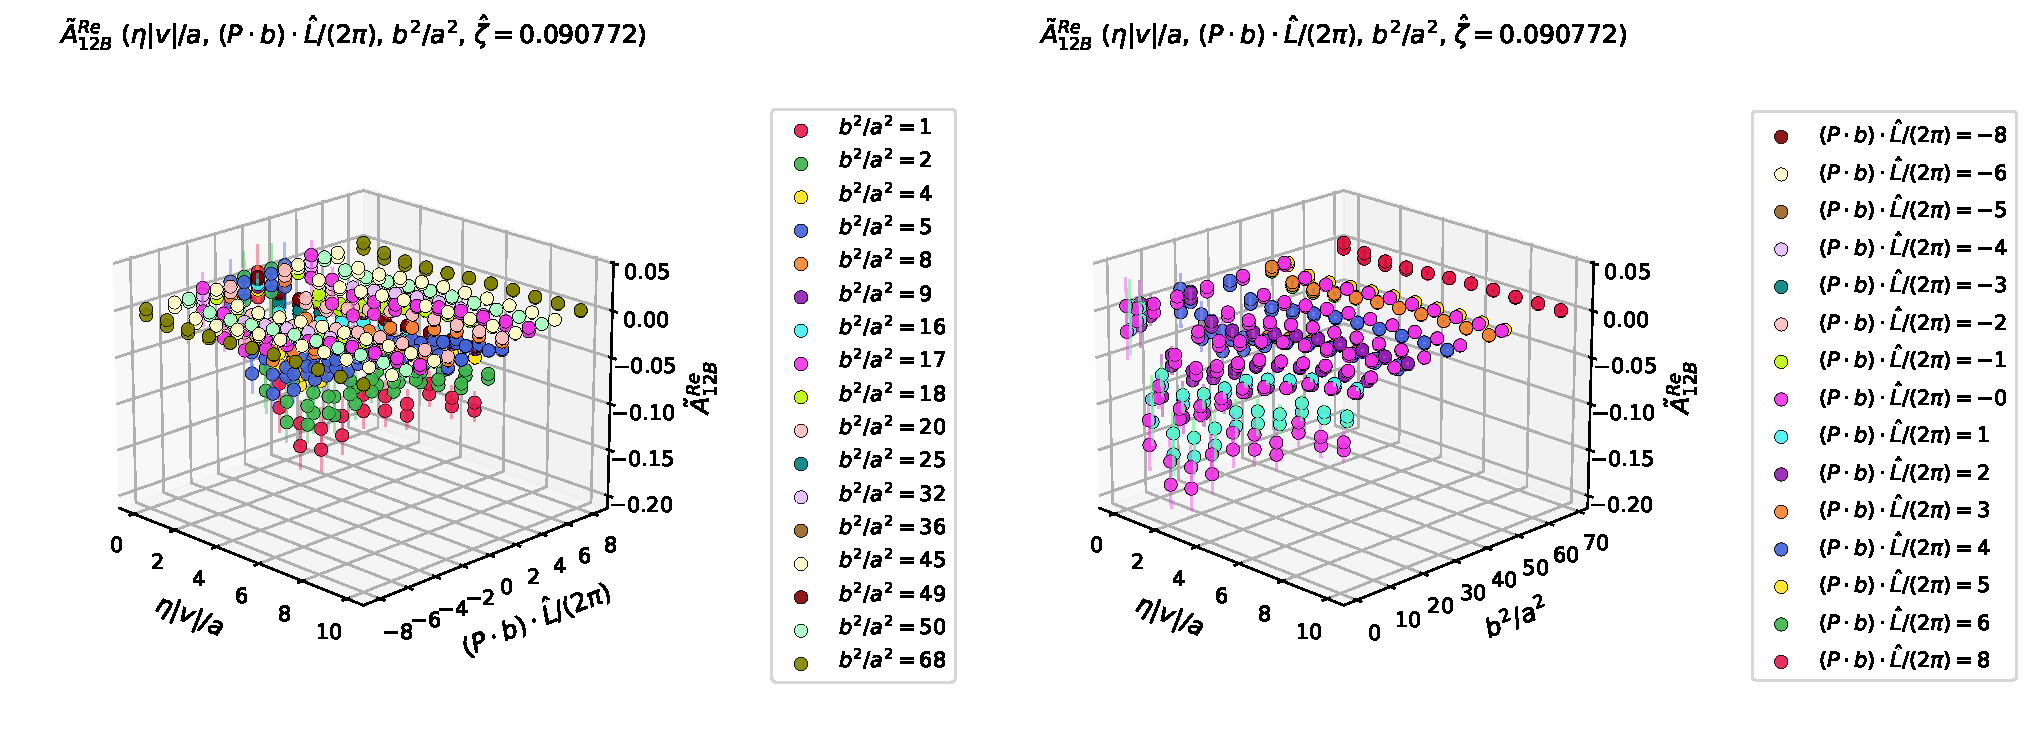
\includegraphics[width=0.98\linewidth,height=0.73\textheight,keepaspectratio]{ReA12B_Pb_bsq_PL-1_3D.pdf}\\[1mm]
{\small $\zetahat=0.090772$; $(\nu,s)$; staple-length dependence}
\figsrc{Thesis, Ch. 5: raw amplitude profiles; complete original panels.}
\end{frame}

\begin{frame}{$\tAmp_{12B}^{\mathrm{Im}}$ at $P_L=-1$: lattice coordinates}
\centering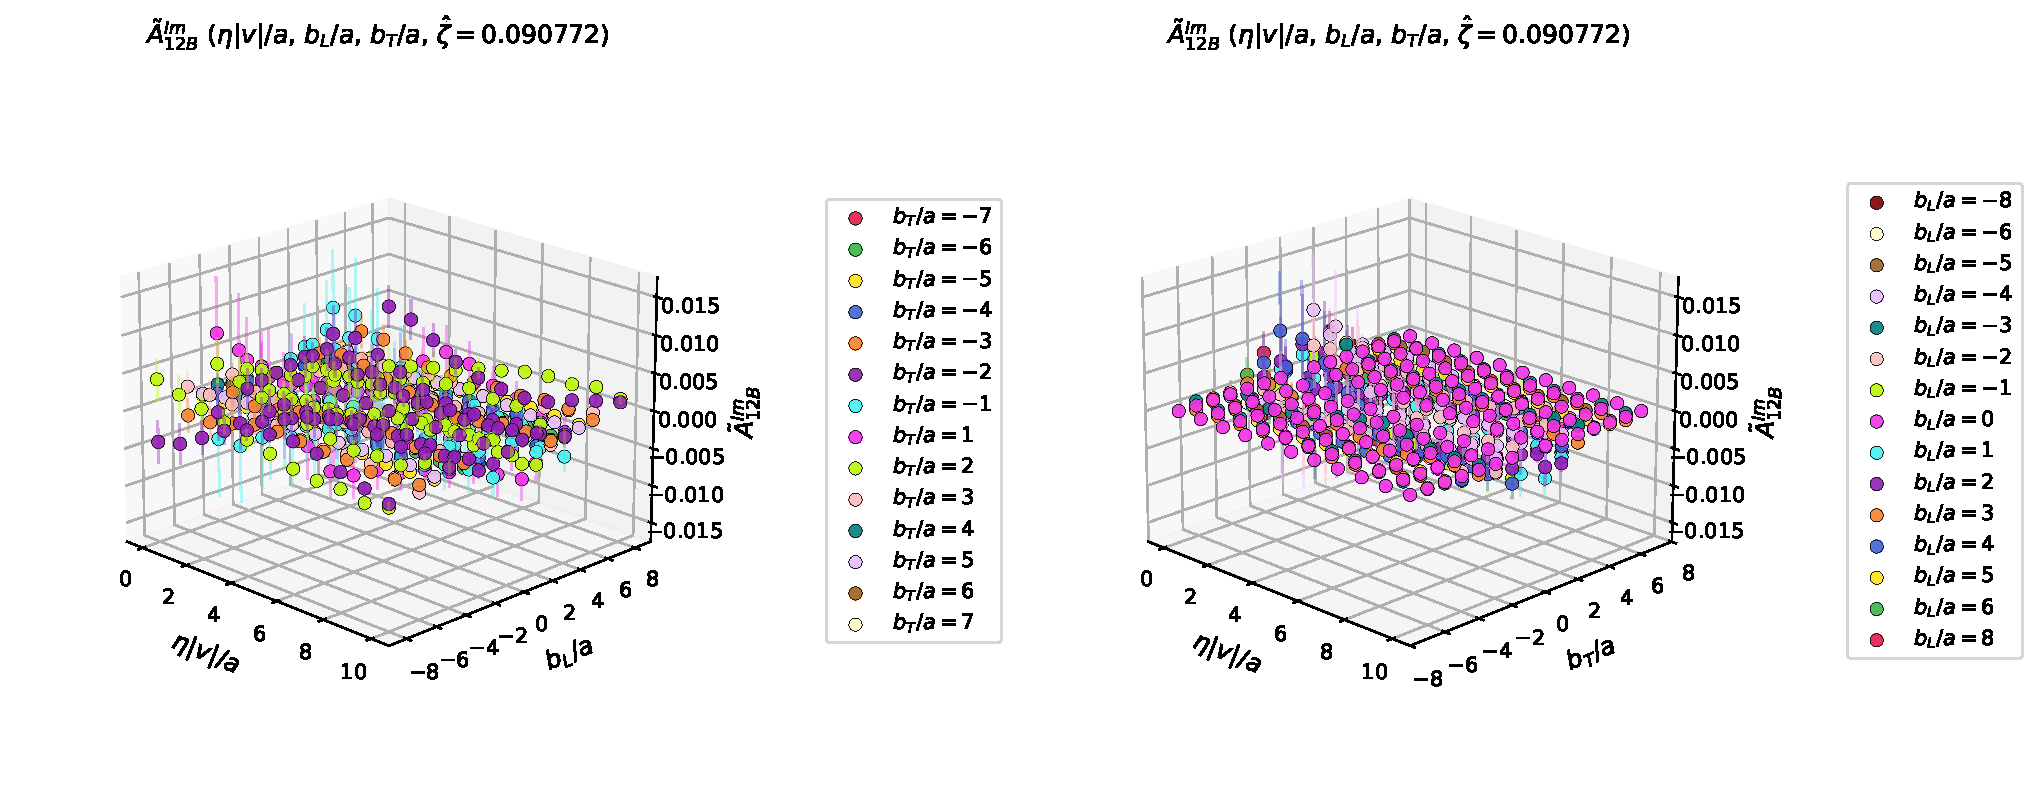
\includegraphics[width=0.98\linewidth,height=0.73\textheight,keepaspectratio]{ImA12B_PL-1_3D.pdf}\\[1mm]
{\small $\zetahat=0.090772$; $(b_L,b_T)$; staple-length dependence}
\figsrc{Thesis, Ch. 5: raw amplitude profiles; complete original panels.}
\end{frame}

\begin{frame}{$\tAmp_{12B}^{\mathrm{Im}}$ at $P_L=-1$: invariant coordinates}
\centering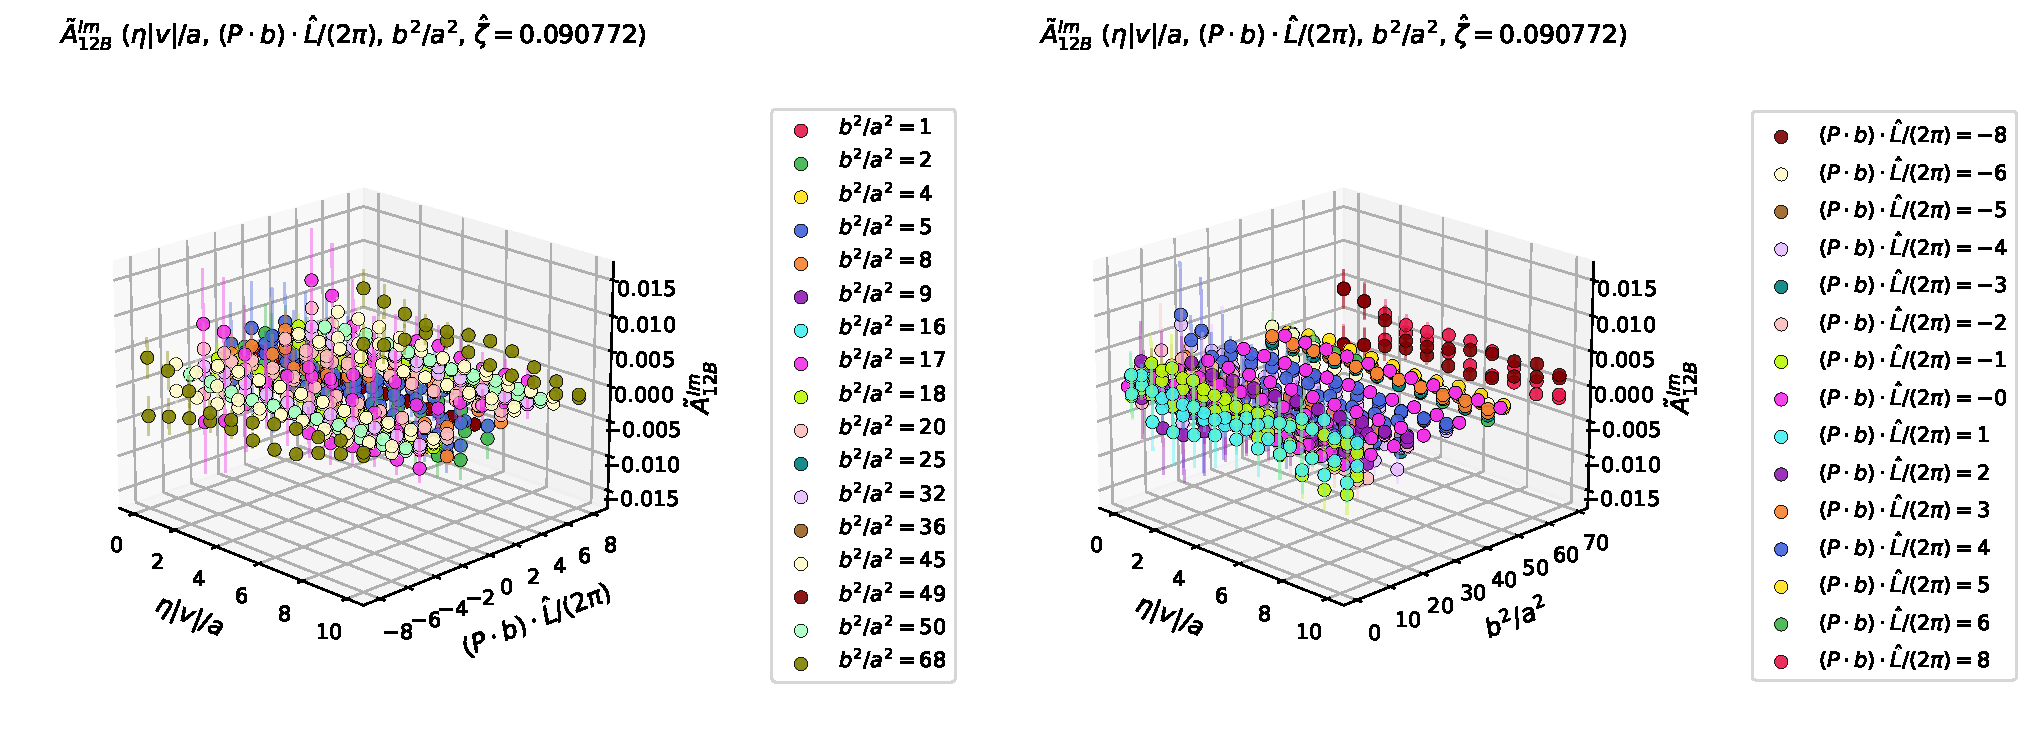
\includegraphics[width=0.98\linewidth,height=0.73\textheight,keepaspectratio]{ImA12B_Pb_bsq_PL-1_3D.pdf}\\[1mm]
{\small $\zetahat=0.090772$; $(\nu,s)$; staple-length dependence}
\figsrc{Thesis, Ch. 5: raw amplitude profiles; complete original panels.}
\end{frame}

\begin{frame}{$\tAmp_{2B}^{\mathrm{Re}}$ at $P_L=-1$: lattice coordinates}
\centering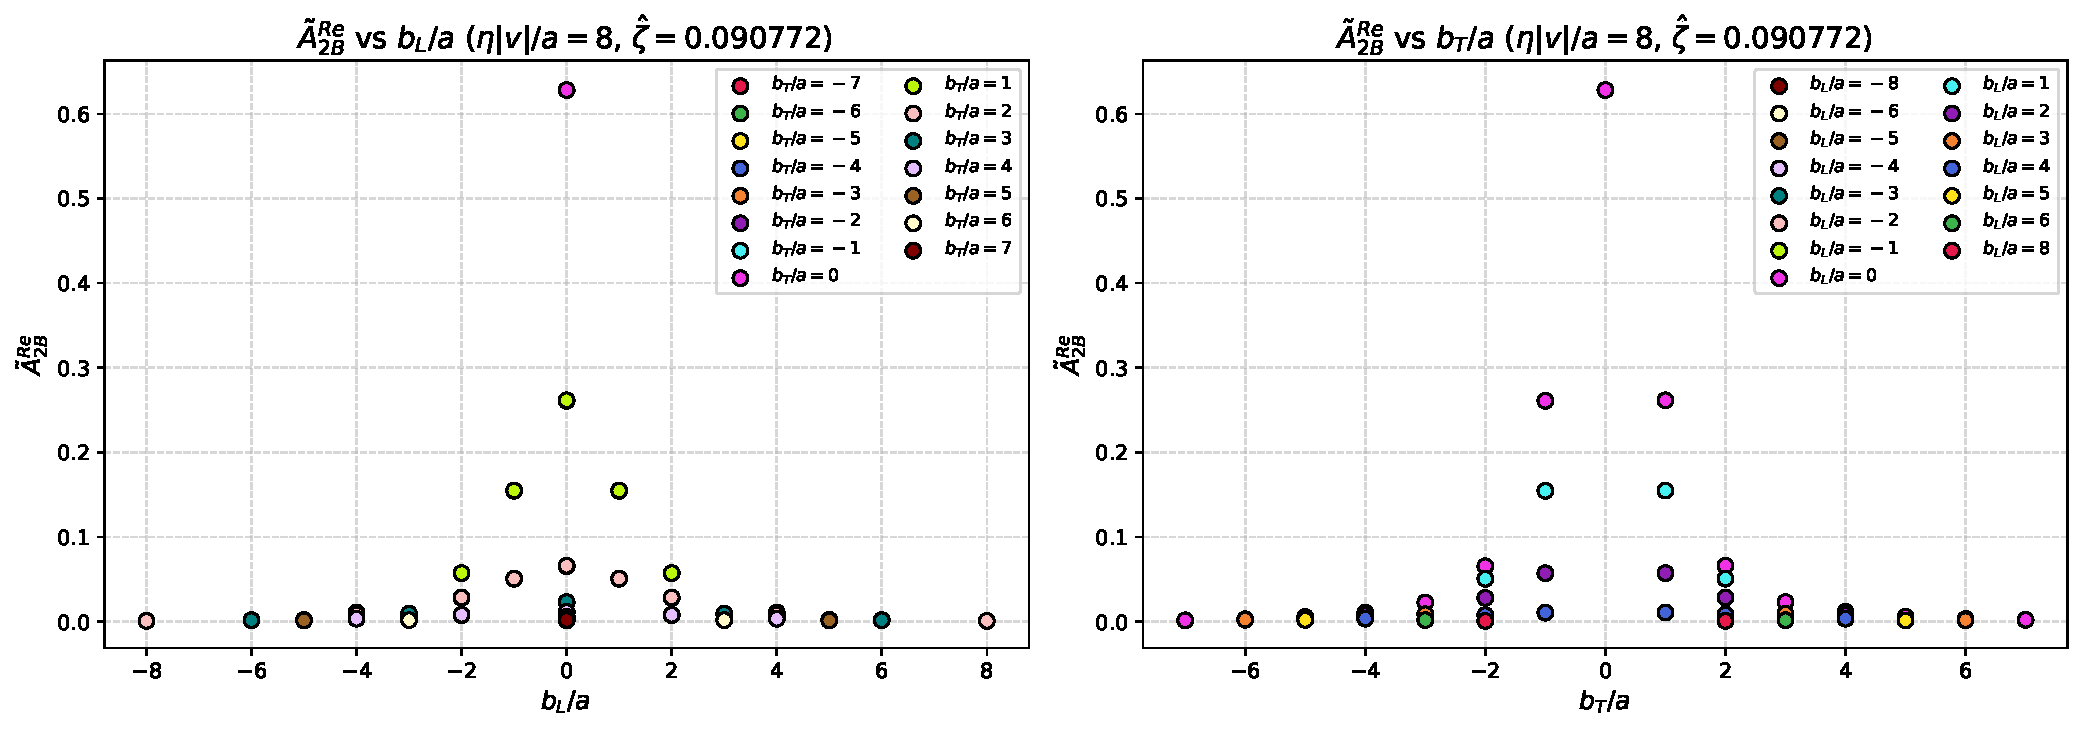
\includegraphics[width=0.98\linewidth,height=0.73\textheight,keepaspectratio]{ReA2B_eta8_PL-1_2D.pdf}\\[1mm]
{\small $\zetahat=0.090772$; $(b_L,b_T)$; $\eta|v|/a=8$ slices}
\figsrc{Thesis, Ch. 5: raw amplitude profiles; complete original panels.}
\end{frame}

\begin{frame}{$\tAmp_{2B}^{\mathrm{Re}}$ at $P_L=-1$: invariant coordinates}
\centering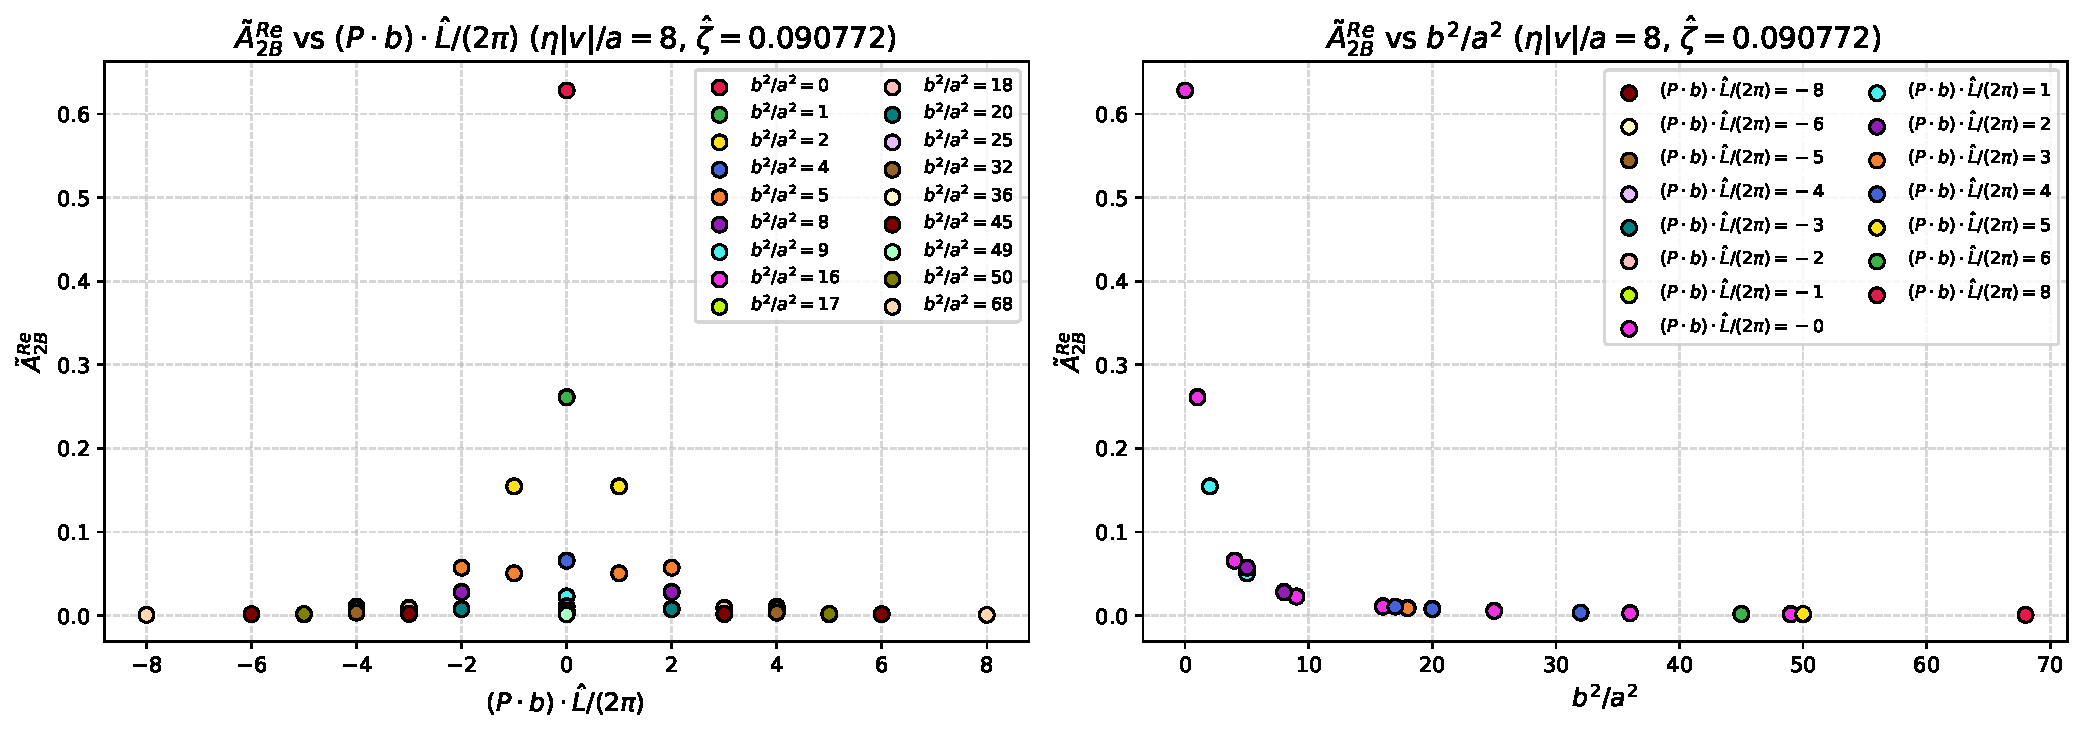
\includegraphics[width=0.98\linewidth,height=0.73\textheight,keepaspectratio]{ReA2B_Pb_bsq_eta8_PL-1_2D.pdf}\\[1mm]
{\small $\zetahat=0.090772$; $(\nu,s)$; $\eta|v|/a=8$ slices}
\figsrc{Thesis, Ch. 5: raw amplitude profiles; complete original panels.}
\end{frame}

\begin{frame}{$\tAmp_{2B}^{\mathrm{Im}}$ at $P_L=-1$: lattice coordinates}
\centering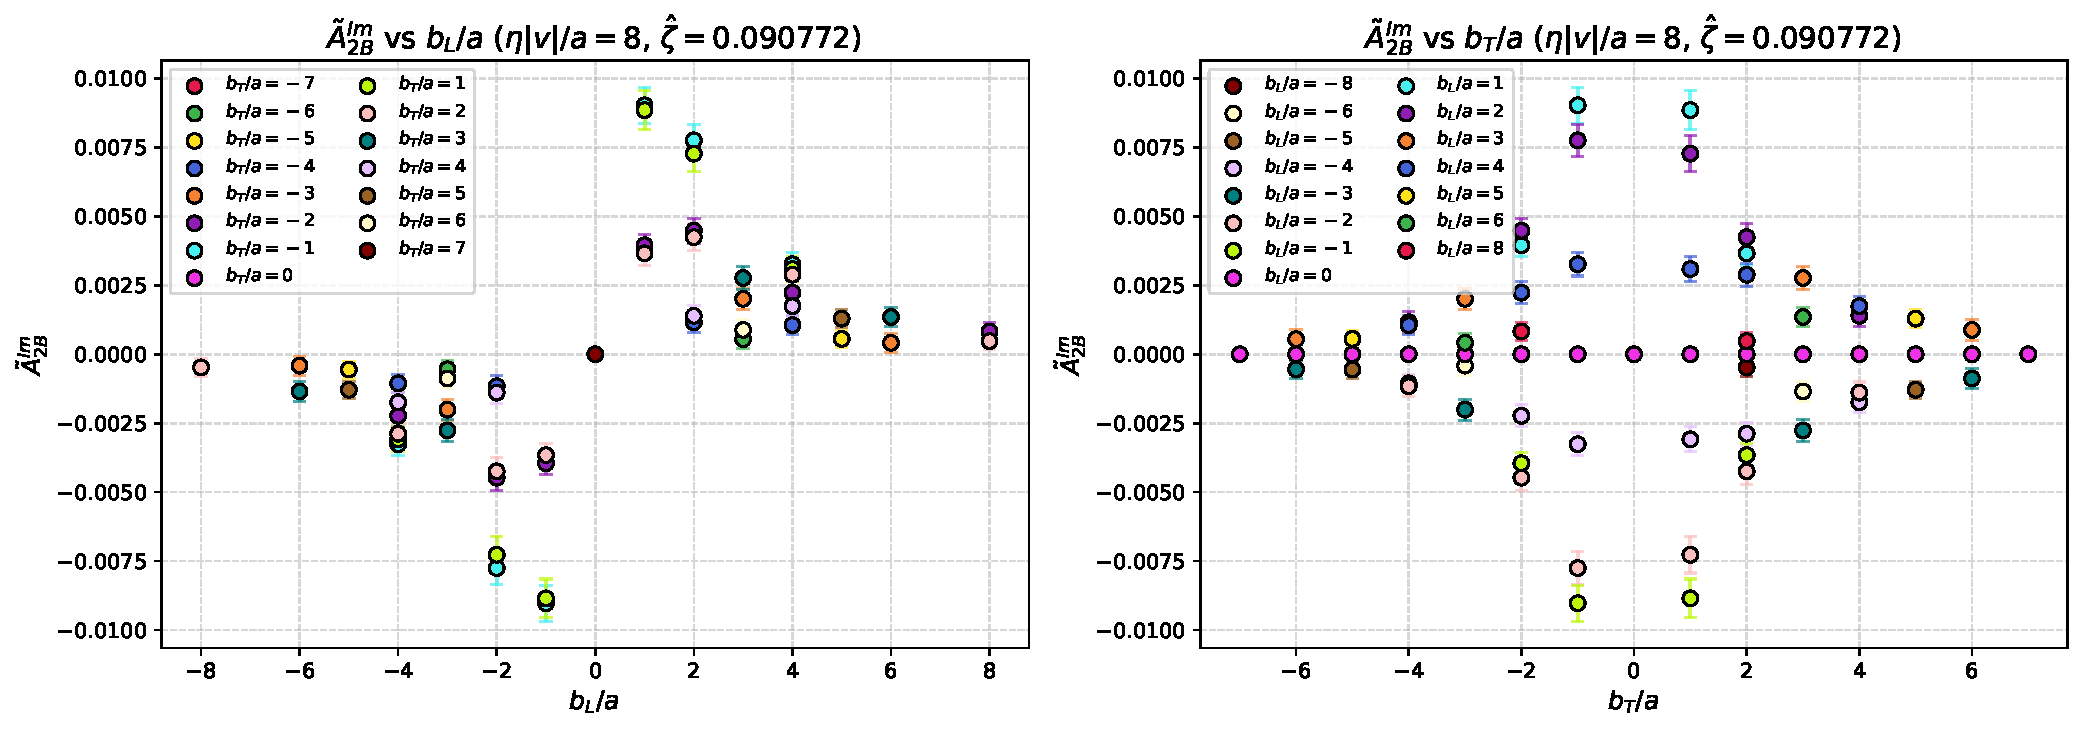
\includegraphics[width=0.98\linewidth,height=0.73\textheight,keepaspectratio]{ImA2B_eta8_PL-1_2D.pdf}\\[1mm]
{\small $\zetahat=0.090772$; $(b_L,b_T)$; $\eta|v|/a=8$ slices}
\figsrc{Thesis, Ch. 5: raw amplitude profiles; complete original panels.}
\end{frame}

\begin{frame}{$\tAmp_{2B}^{\mathrm{Im}}$ at $P_L=-1$: invariant coordinates}
\centering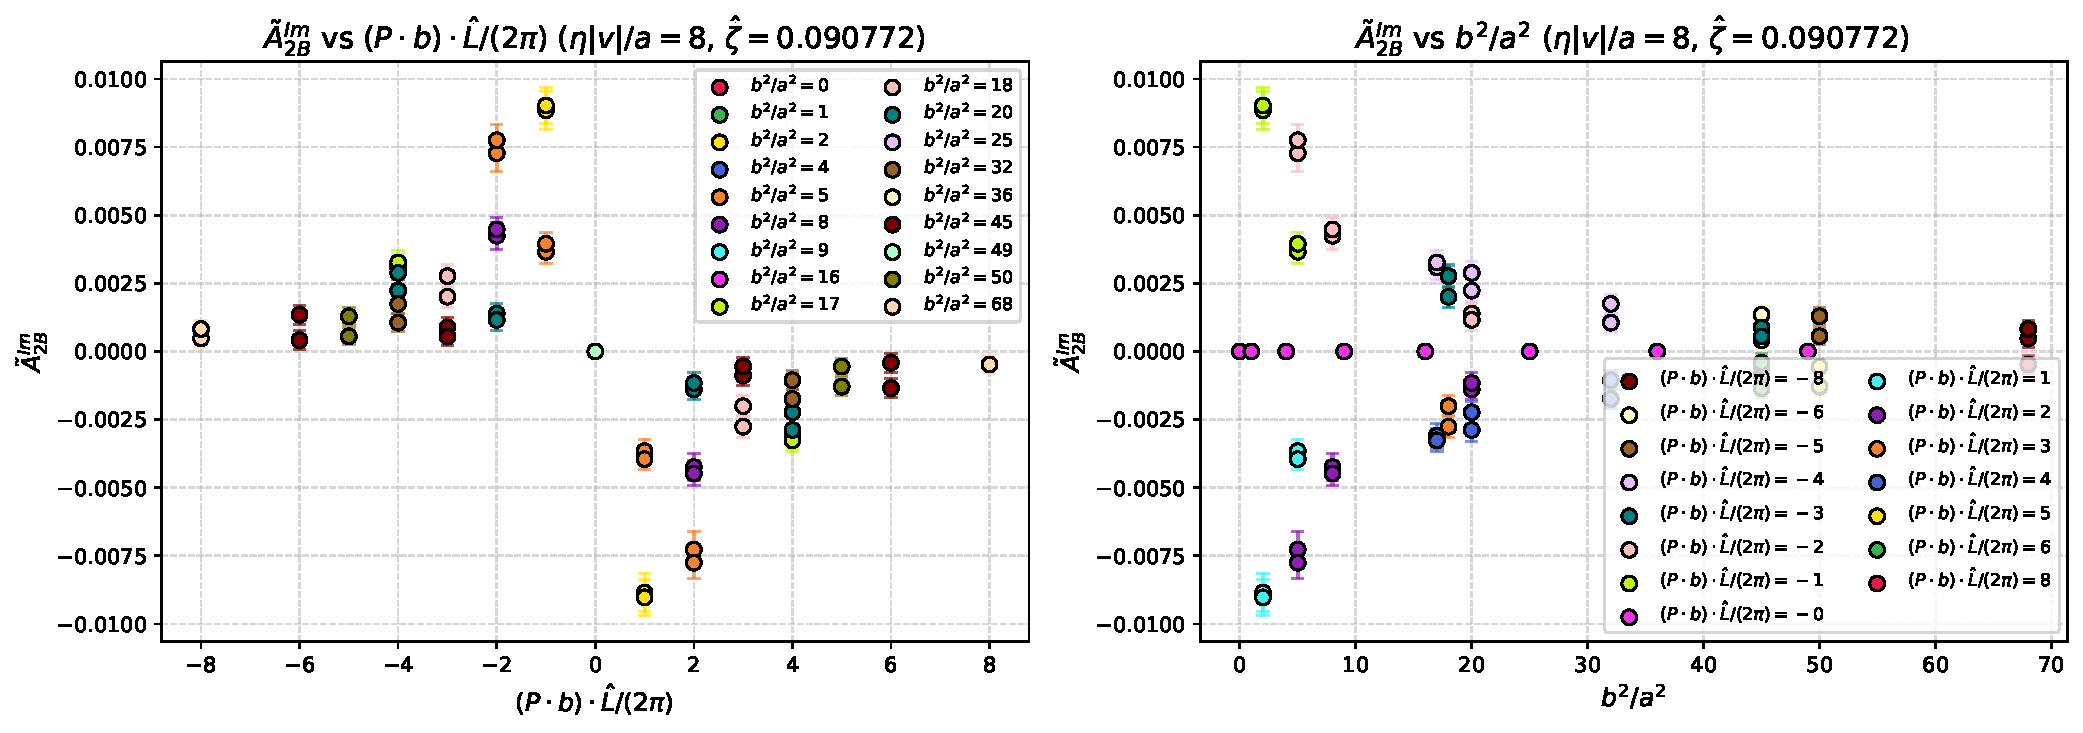
\includegraphics[width=0.98\linewidth,height=0.73\textheight,keepaspectratio]{ImA2B_Pb_bsq_eta8_PL-1_2D.pdf}\\[1mm]
{\small $\zetahat=0.090772$; $(\nu,s)$; $\eta|v|/a=8$ slices}
\figsrc{Thesis, Ch. 5: raw amplitude profiles; complete original panels.}
\end{frame}

\begin{frame}{$\tAmp_{12B}^{\mathrm{Re}}$ at $P_L=-1$: lattice coordinates}
\centering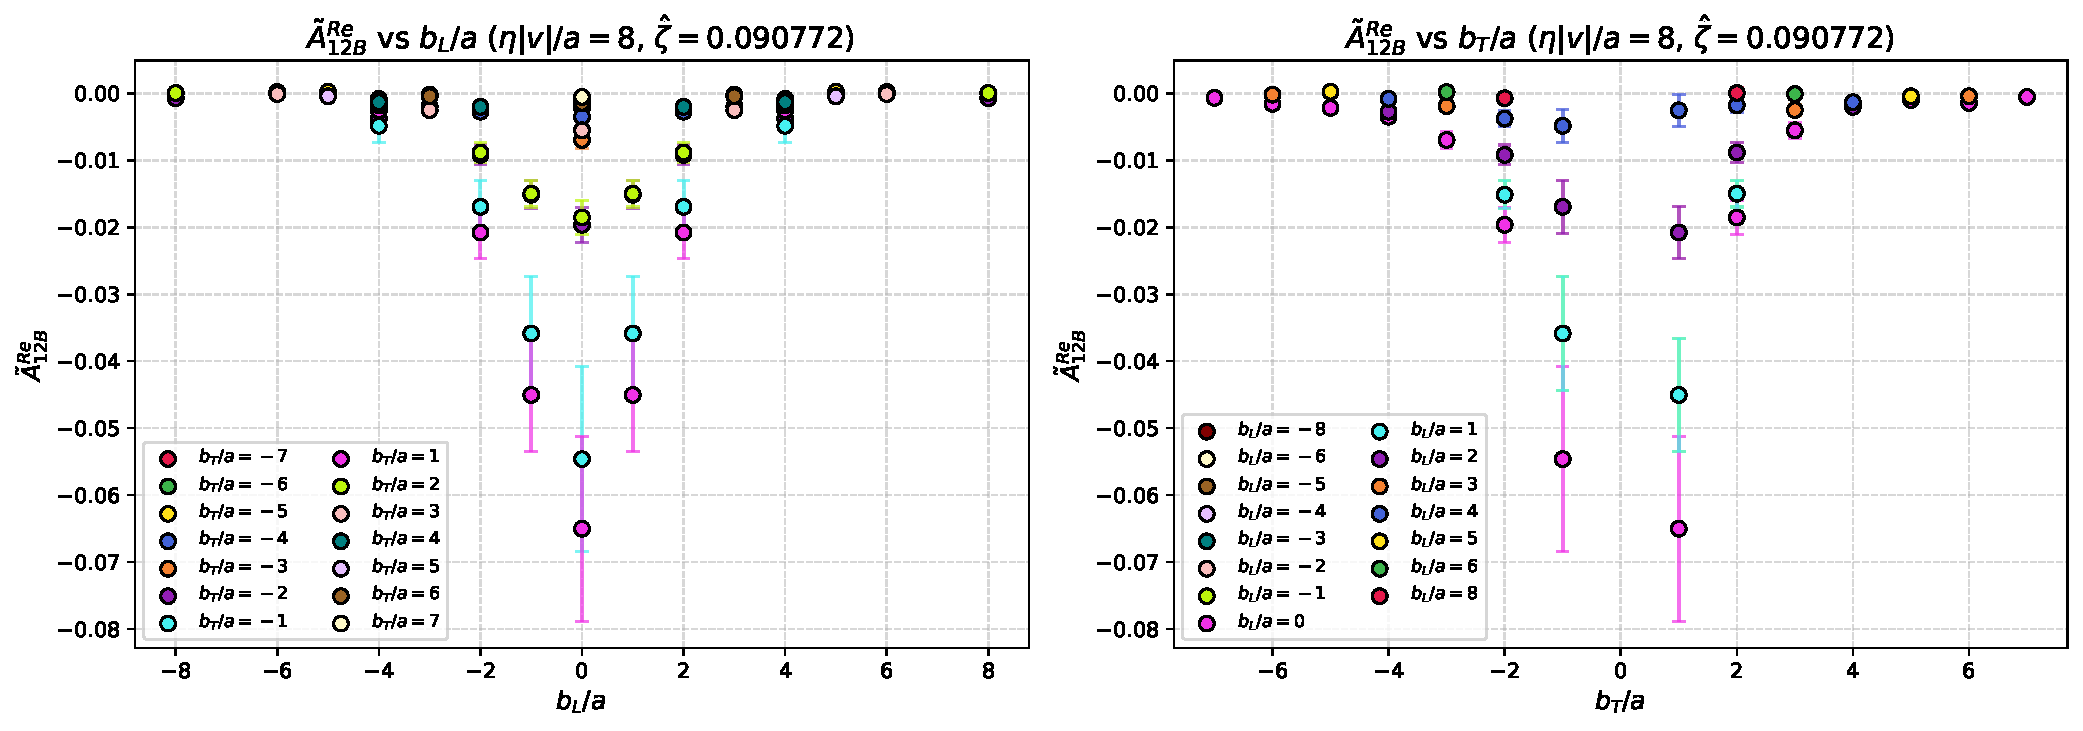
\includegraphics[width=0.98\linewidth,height=0.73\textheight,keepaspectratio]{ReA12B_eta8_PL-1_2D.pdf}\\[1mm]
{\small $\zetahat=0.090772$; $(b_L,b_T)$; $\eta|v|/a=8$ slices}
\figsrc{Thesis, Ch. 5: raw amplitude profiles; complete original panels.}
\end{frame}

\begin{frame}{$\tAmp_{12B}^{\mathrm{Re}}$ at $P_L=-1$: invariant coordinates}
\centering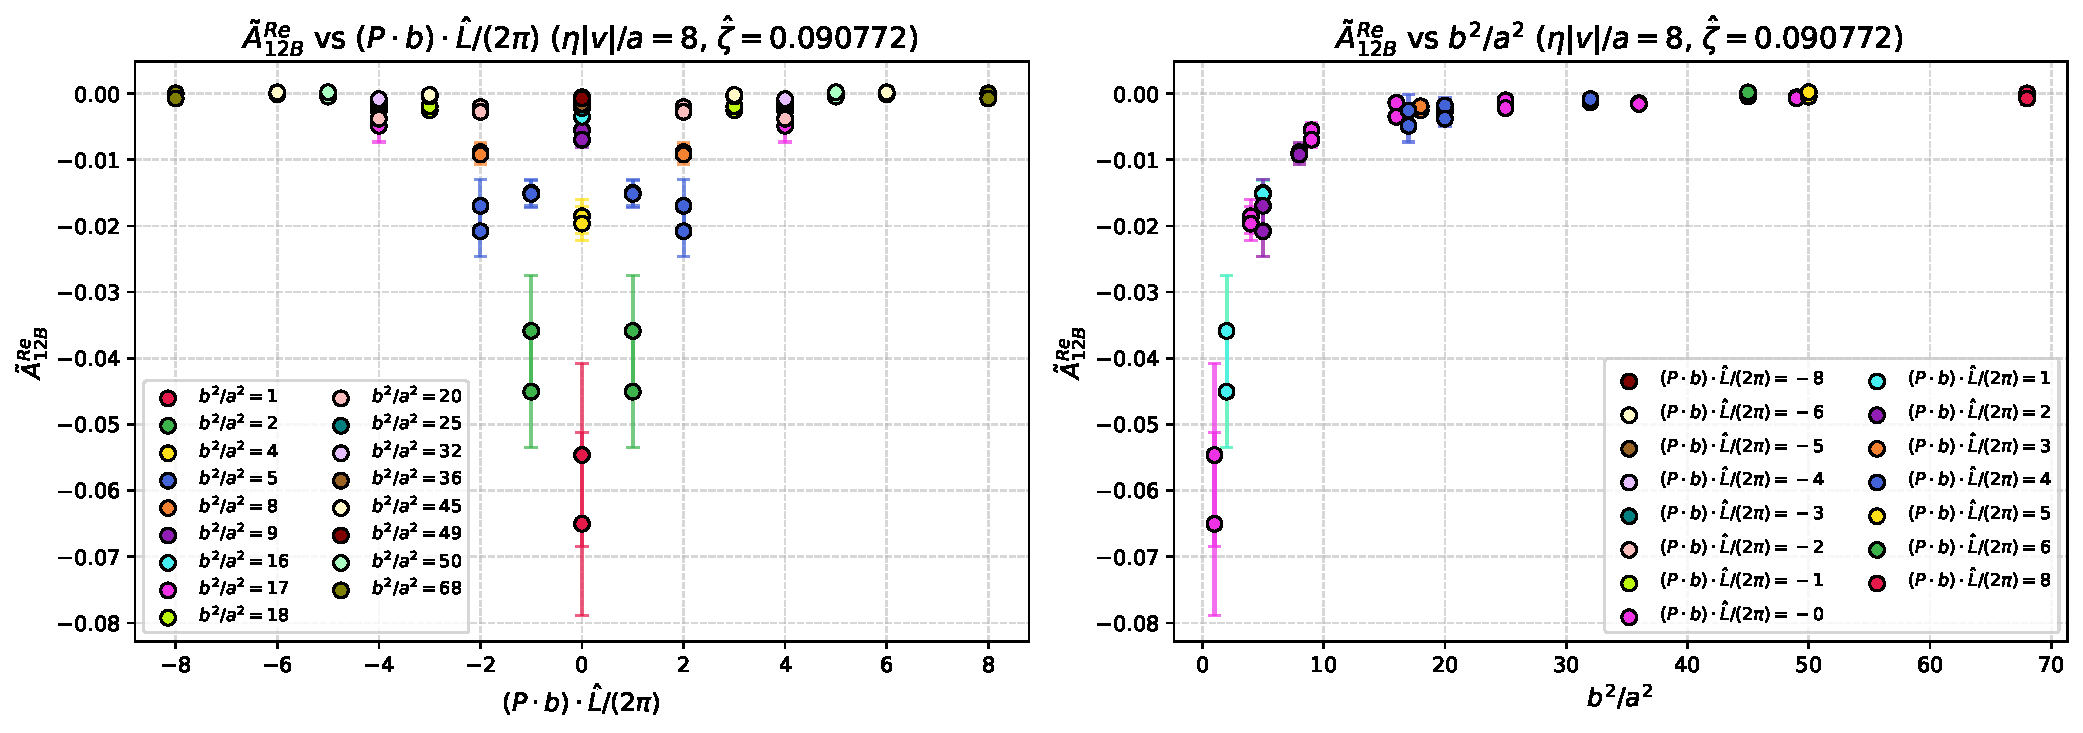
\includegraphics[width=0.98\linewidth,height=0.73\textheight,keepaspectratio]{ReA12B_Pb_bsq_eta8_PL-1_2D.pdf}\\[1mm]
{\small $\zetahat=0.090772$; $(\nu,s)$; $\eta|v|/a=8$ slices}
\figsrc{Thesis, Ch. 5: raw amplitude profiles; complete original panels.}
\end{frame}

\begin{frame}{$\tAmp_{12B}^{\mathrm{Im}}$ at $P_L=-1$: lattice coordinates}
\centering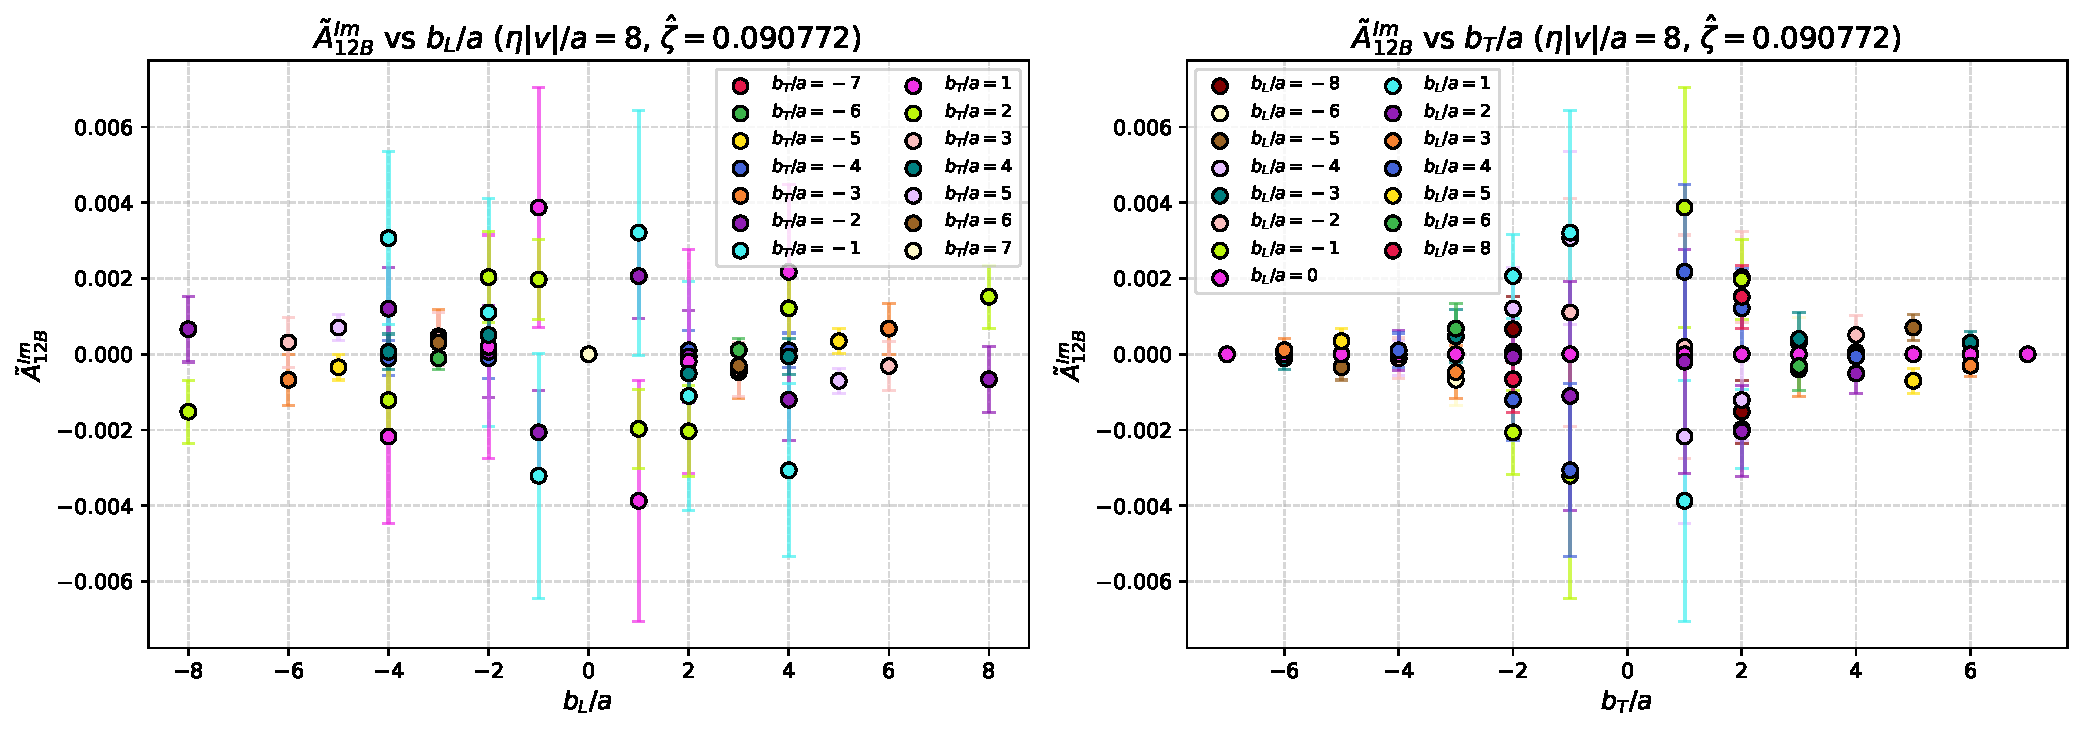
\includegraphics[width=0.98\linewidth,height=0.73\textheight,keepaspectratio]{ImA12B_eta8_PL-1_2D.pdf}\\[1mm]
{\small $\zetahat=0.090772$; $(b_L,b_T)$; $\eta|v|/a=8$ slices}
\figsrc{Thesis, Ch. 5: raw amplitude profiles; complete original panels.}
\end{frame}

\begin{frame}{$\tAmp_{12B}^{\mathrm{Im}}$ at $P_L=-1$: invariant coordinates}
\centering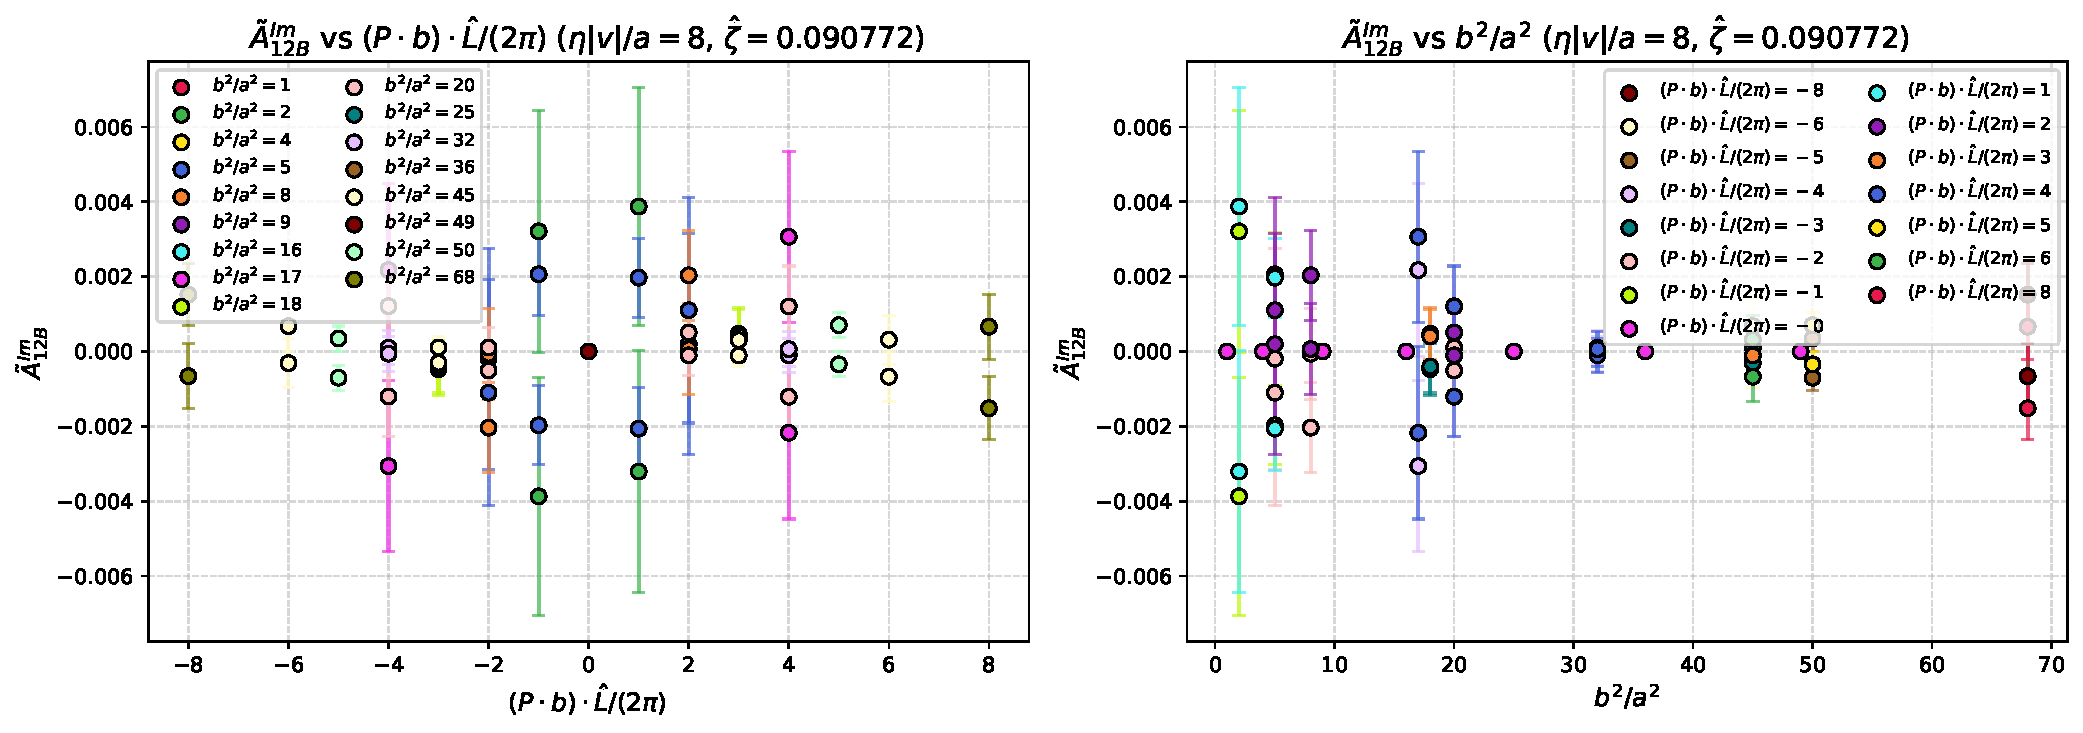
\includegraphics[width=0.98\linewidth,height=0.73\textheight,keepaspectratio]{ImA12B_Pb_bsq_eta8_PL-1_2D.pdf}\\[1mm]
{\small $\zetahat=0.090772$; $(\nu,s)$; $\eta|v|/a=8$ slices}
\figsrc{Thesis, Ch. 5: raw amplitude profiles; complete original panels.}
\end{frame}

\begin{frame}{$\tAmp_{2B}^{\mathrm{Re}}$ at $P_L=-2$: lattice coordinates}
\centering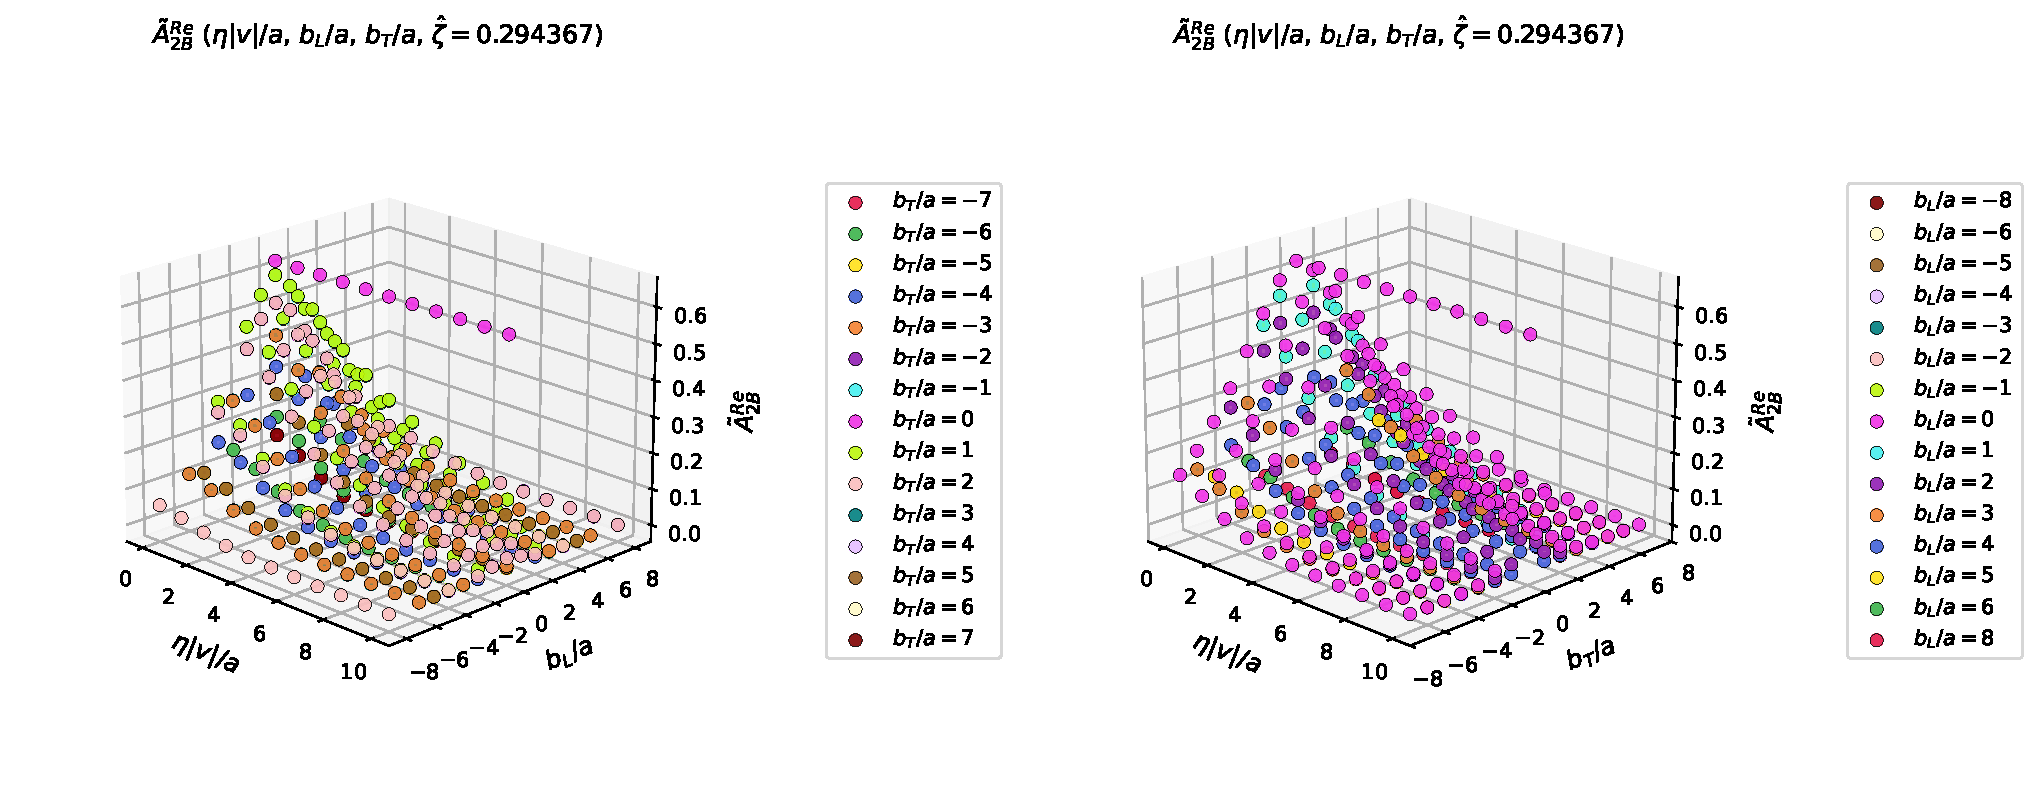
\includegraphics[width=0.98\linewidth,height=0.73\textheight,keepaspectratio]{ReA2B_PL-2_3D.pdf}\\[1mm]
{\small $\zetahat=0.294367$; $(b_L,b_T)$; staple-length dependence}
\figsrc{Thesis, Ch. 5: raw amplitude profiles; complete original panels.}
\end{frame}

\begin{frame}{$\tAmp_{2B}^{\mathrm{Re}}$ at $P_L=-2$: invariant coordinates}
\centering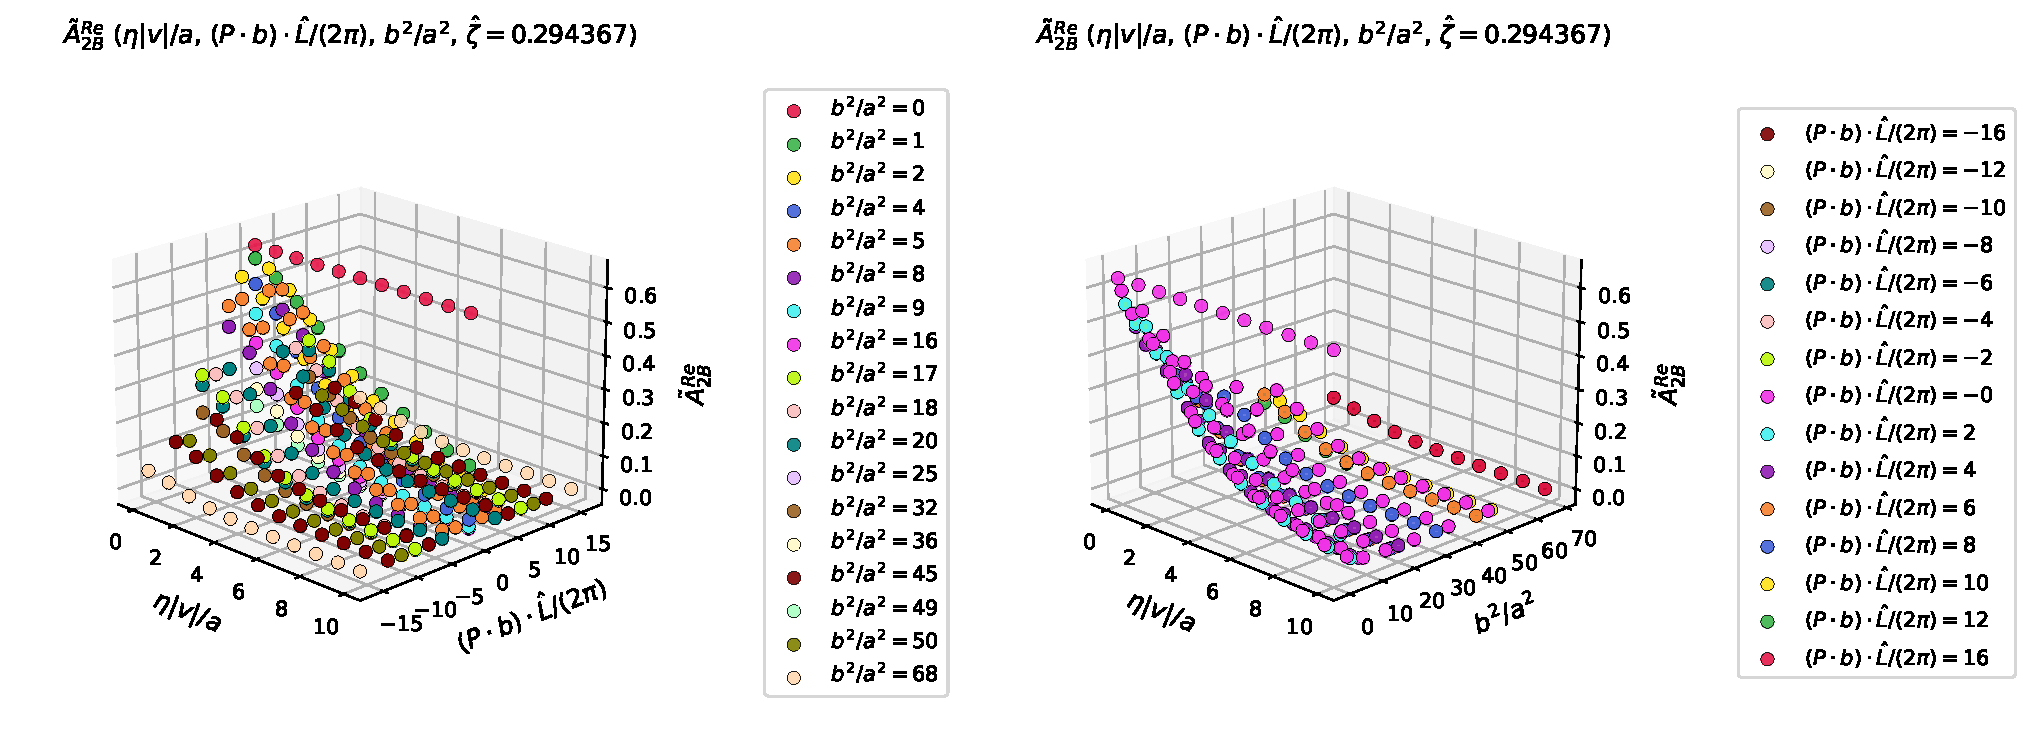
\includegraphics[width=0.98\linewidth,height=0.73\textheight,keepaspectratio]{ReA2B_Pb_bsq_PL-2_3D.pdf}\\[1mm]
{\small $\zetahat=0.294367$; $(\nu,s)$; staple-length dependence}
\figsrc{Thesis, Ch. 5: raw amplitude profiles; complete original panels.}
\end{frame}

\begin{frame}{$\tAmp_{2B}^{\mathrm{Im}}$ at $P_L=-2$: lattice coordinates}
\centering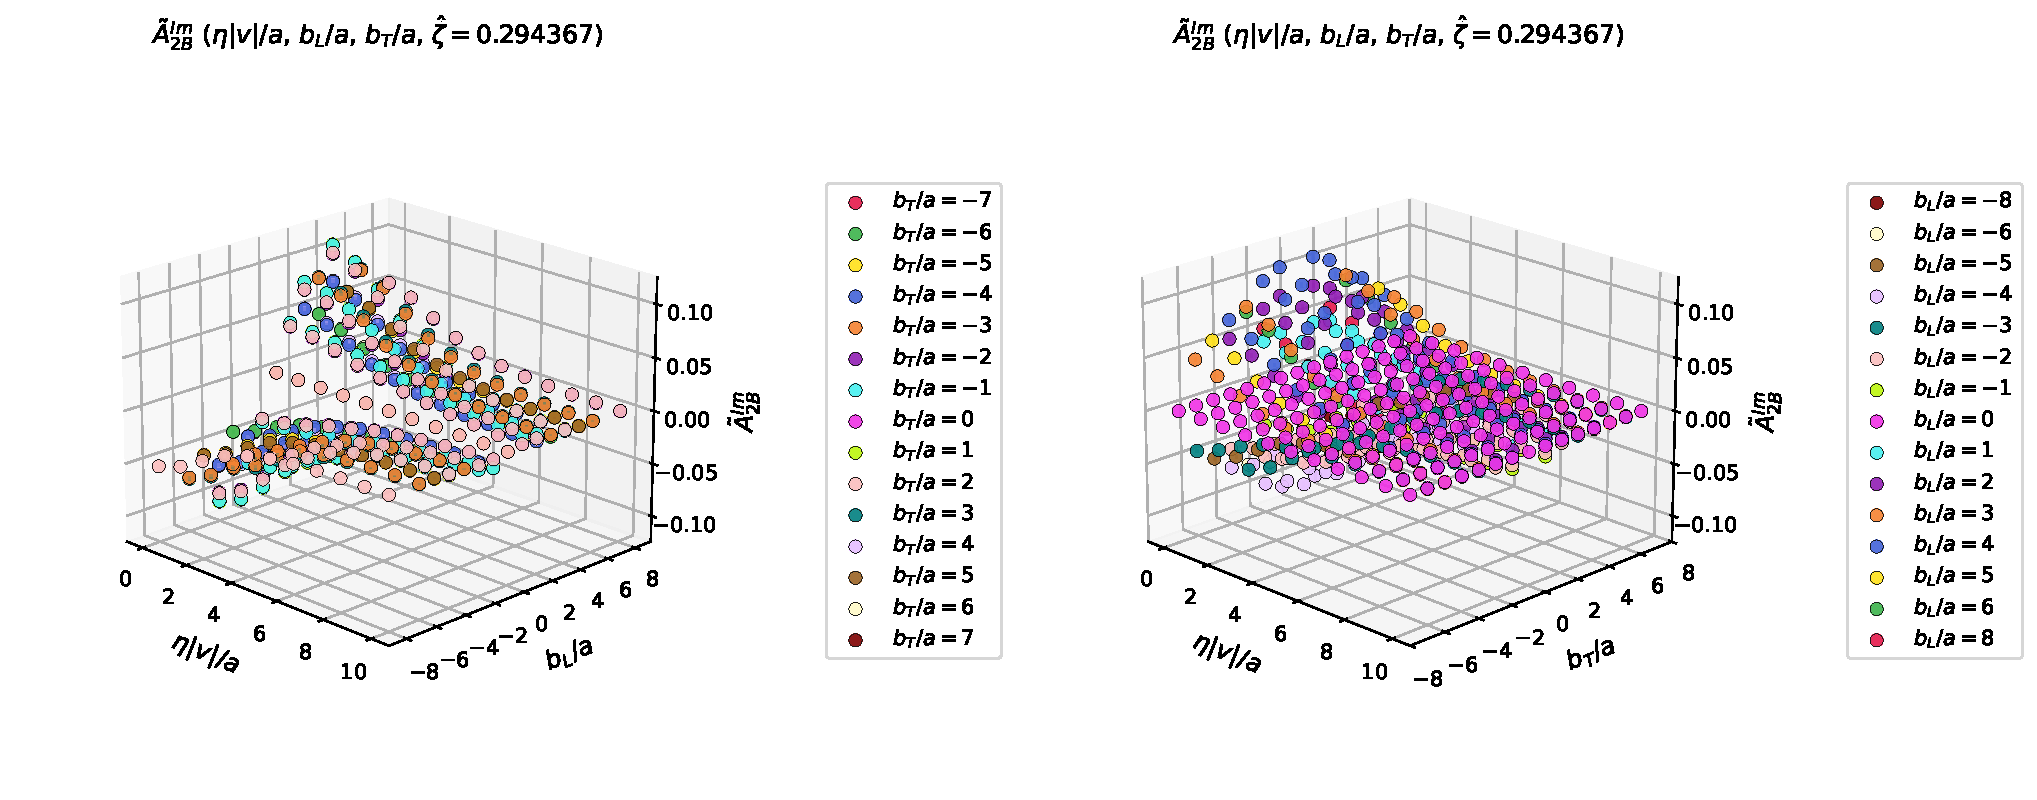
\includegraphics[width=0.98\linewidth,height=0.73\textheight,keepaspectratio]{ImA2B_PL-2_3D.pdf}\\[1mm]
{\small $\zetahat=0.294367$; $(b_L,b_T)$; staple-length dependence}
\figsrc{Thesis, Ch. 5: raw amplitude profiles; complete original panels.}
\end{frame}

\begin{frame}{$\tAmp_{2B}^{\mathrm{Im}}$ at $P_L=-2$: invariant coordinates}
\centering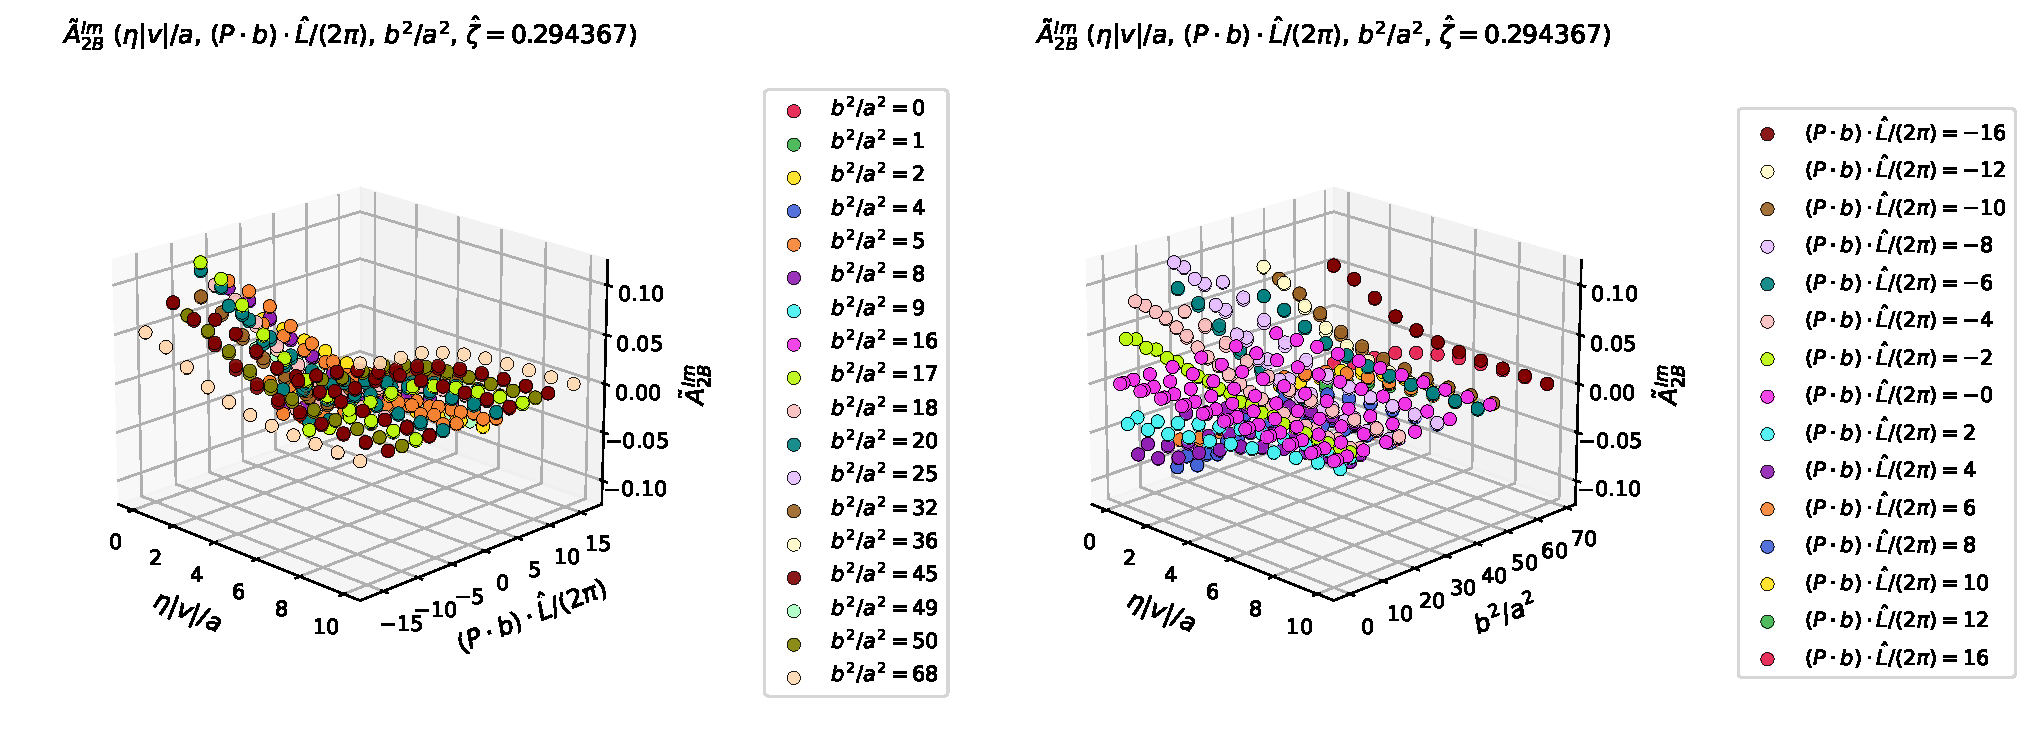
\includegraphics[width=0.98\linewidth,height=0.73\textheight,keepaspectratio]{ImA2B_Pb_bsq_PL-2_3D.pdf}\\[1mm]
{\small $\zetahat=0.294367$; $(\nu,s)$; staple-length dependence}
\figsrc{Thesis, Ch. 5: raw amplitude profiles; complete original panels.}
\end{frame}

\begin{frame}{$\tAmp_{12B}^{\mathrm{Re}}$ at $P_L=-2$: lattice coordinates}
\centering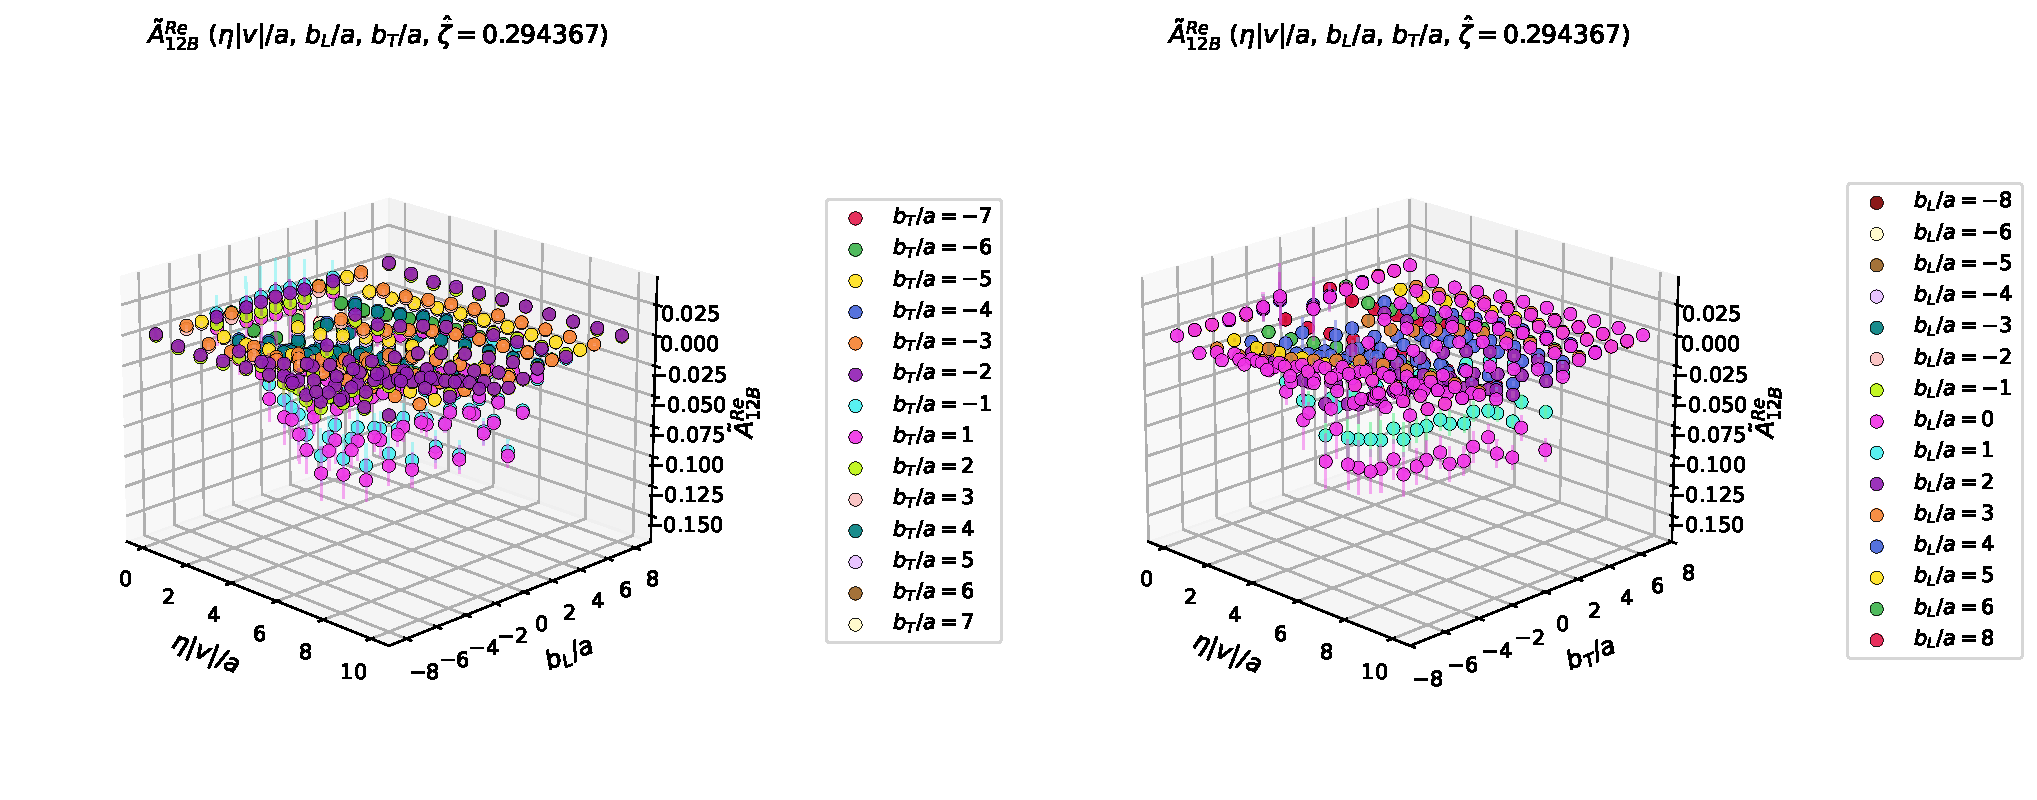
\includegraphics[width=0.98\linewidth,height=0.73\textheight,keepaspectratio]{ReA12B_PL-2_3D.pdf}\\[1mm]
{\small $\zetahat=0.294367$; $(b_L,b_T)$; staple-length dependence}
\figsrc{Thesis, Ch. 5: raw amplitude profiles; complete original panels.}
\end{frame}

\begin{frame}{$\tAmp_{12B}^{\mathrm{Re}}$ at $P_L=-2$: invariant coordinates}
\centering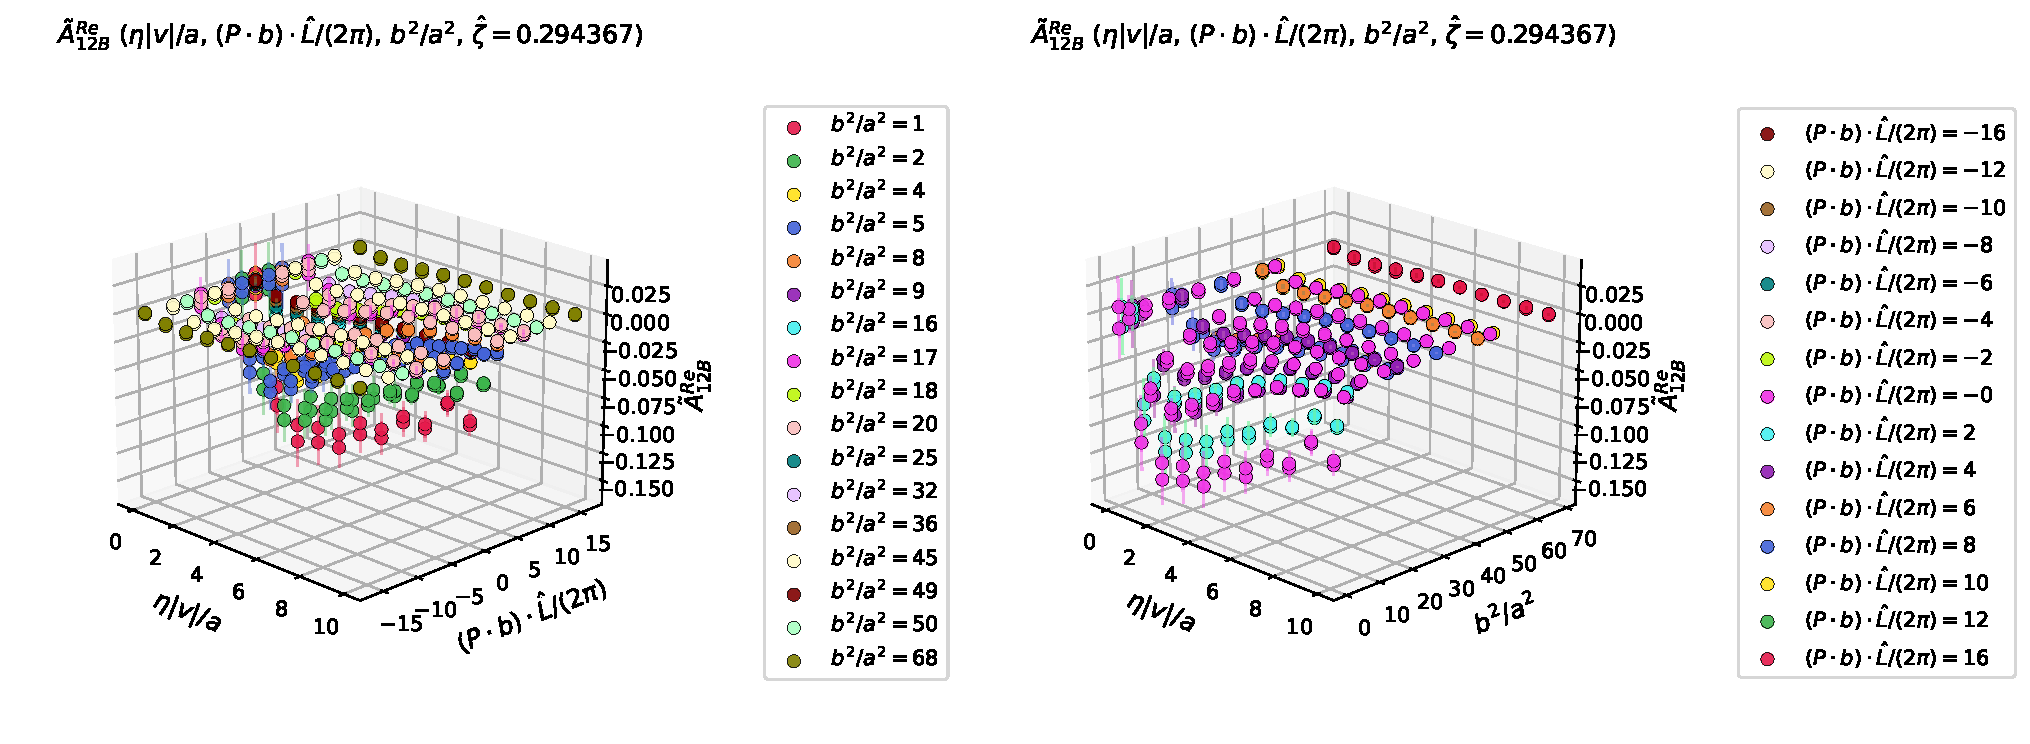
\includegraphics[width=0.98\linewidth,height=0.73\textheight,keepaspectratio]{ReA12B_Pb_bsq_PL-2_3D.pdf}\\[1mm]
{\small $\zetahat=0.294367$; $(\nu,s)$; staple-length dependence}
\figsrc{Thesis, Ch. 5: raw amplitude profiles; complete original panels.}
\end{frame}

\begin{frame}{$\tAmp_{12B}^{\mathrm{Im}}$ at $P_L=-2$: lattice coordinates}
\centering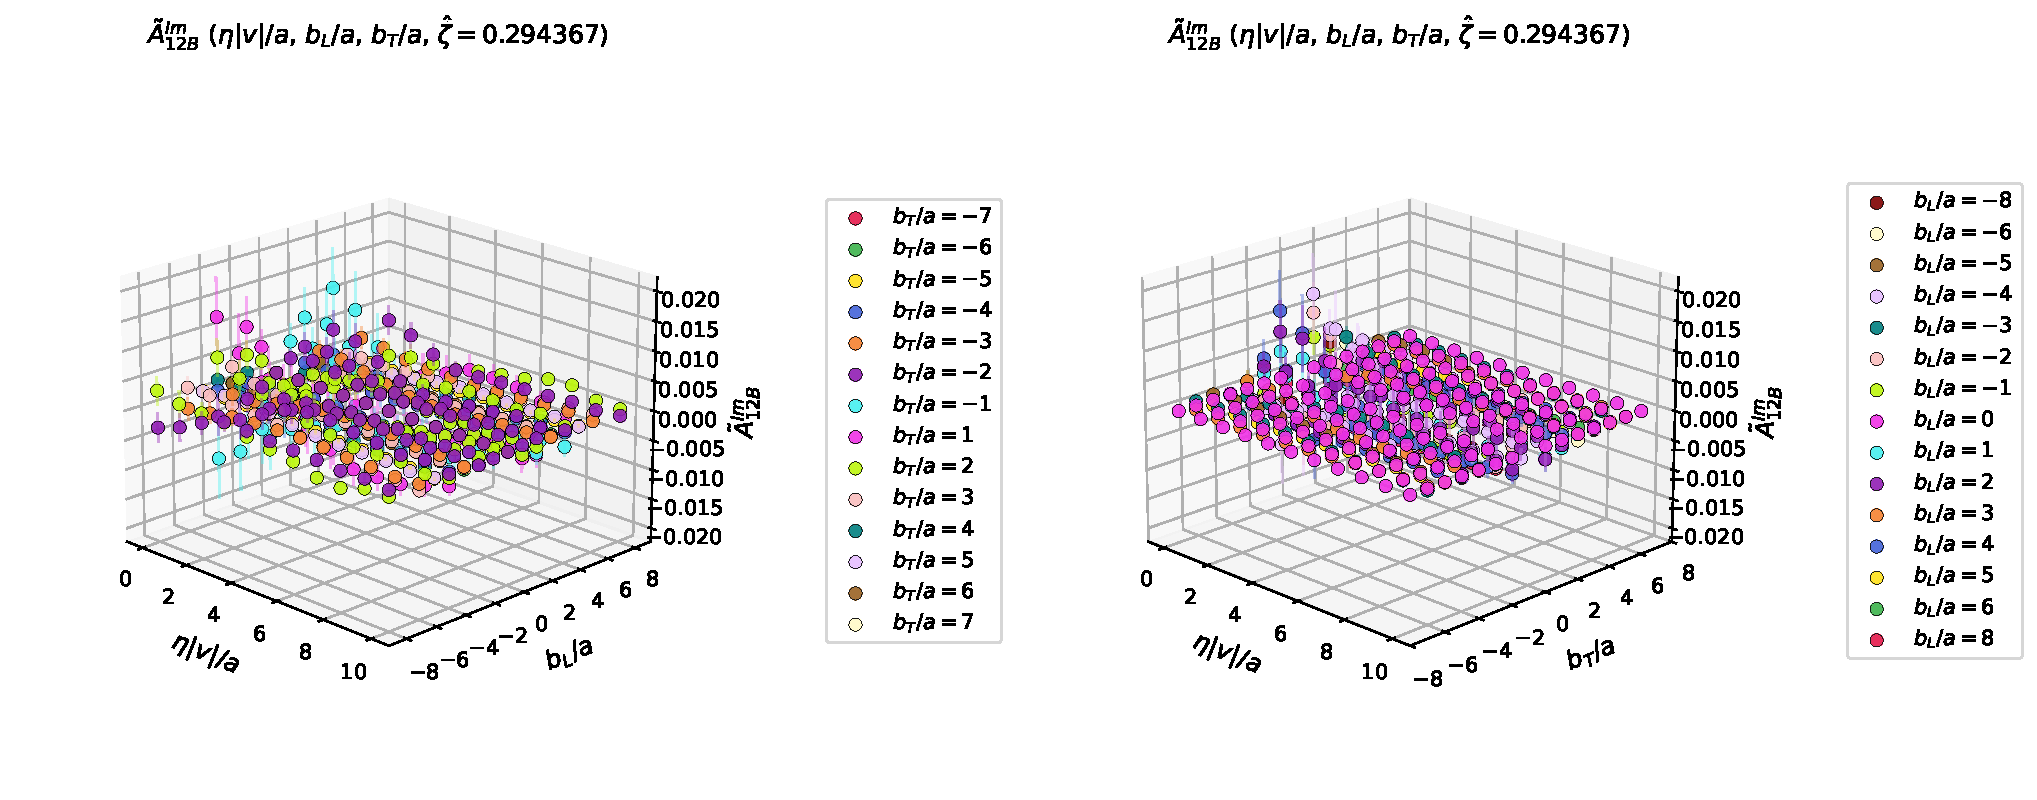
\includegraphics[width=0.98\linewidth,height=0.73\textheight,keepaspectratio]{ImA12B_PL-2_3D.pdf}\\[1mm]
{\small $\zetahat=0.294367$; $(b_L,b_T)$; staple-length dependence}
\figsrc{Thesis, Ch. 5: raw amplitude profiles; complete original panels.}
\end{frame}

\begin{frame}{$\tAmp_{12B}^{\mathrm{Im}}$ at $P_L=-2$: invariant coordinates}
\centering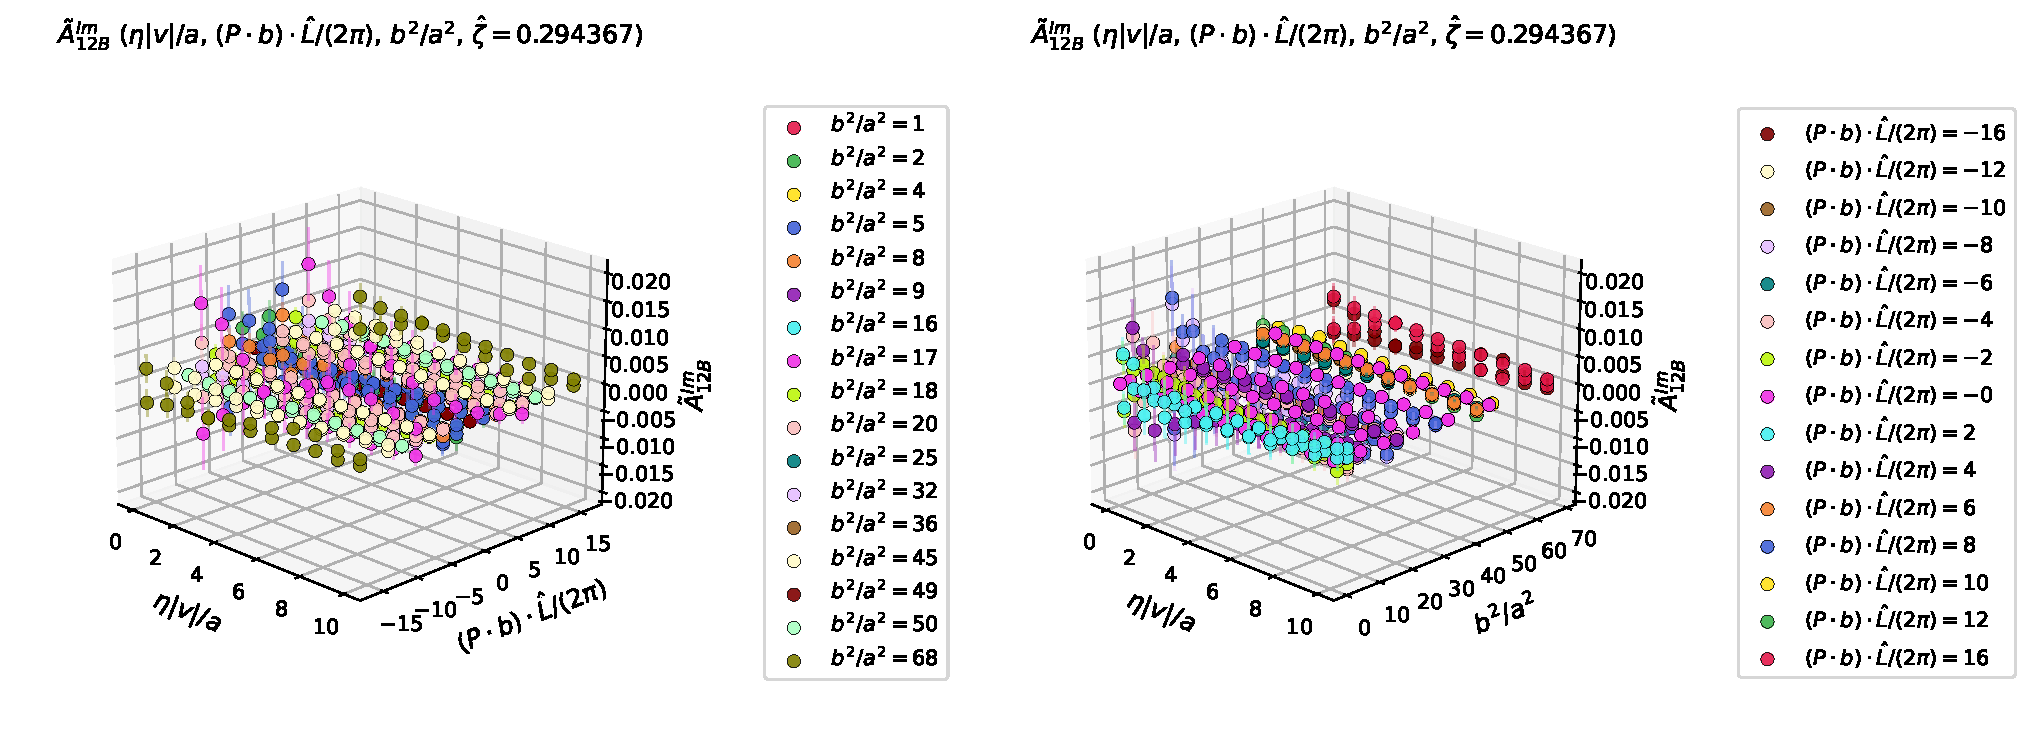
\includegraphics[width=0.98\linewidth,height=0.73\textheight,keepaspectratio]{ImA12B_Pb_bsq_PL-2_3D.pdf}\\[1mm]
{\small $\zetahat=0.294367$; $(\nu,s)$; staple-length dependence}
\figsrc{Thesis, Ch. 5: raw amplitude profiles; complete original panels.}
\end{frame}

\begin{frame}{$\tAmp_{2B}^{\mathrm{Re}}$ at $P_L=-2$: lattice coordinates}
\centering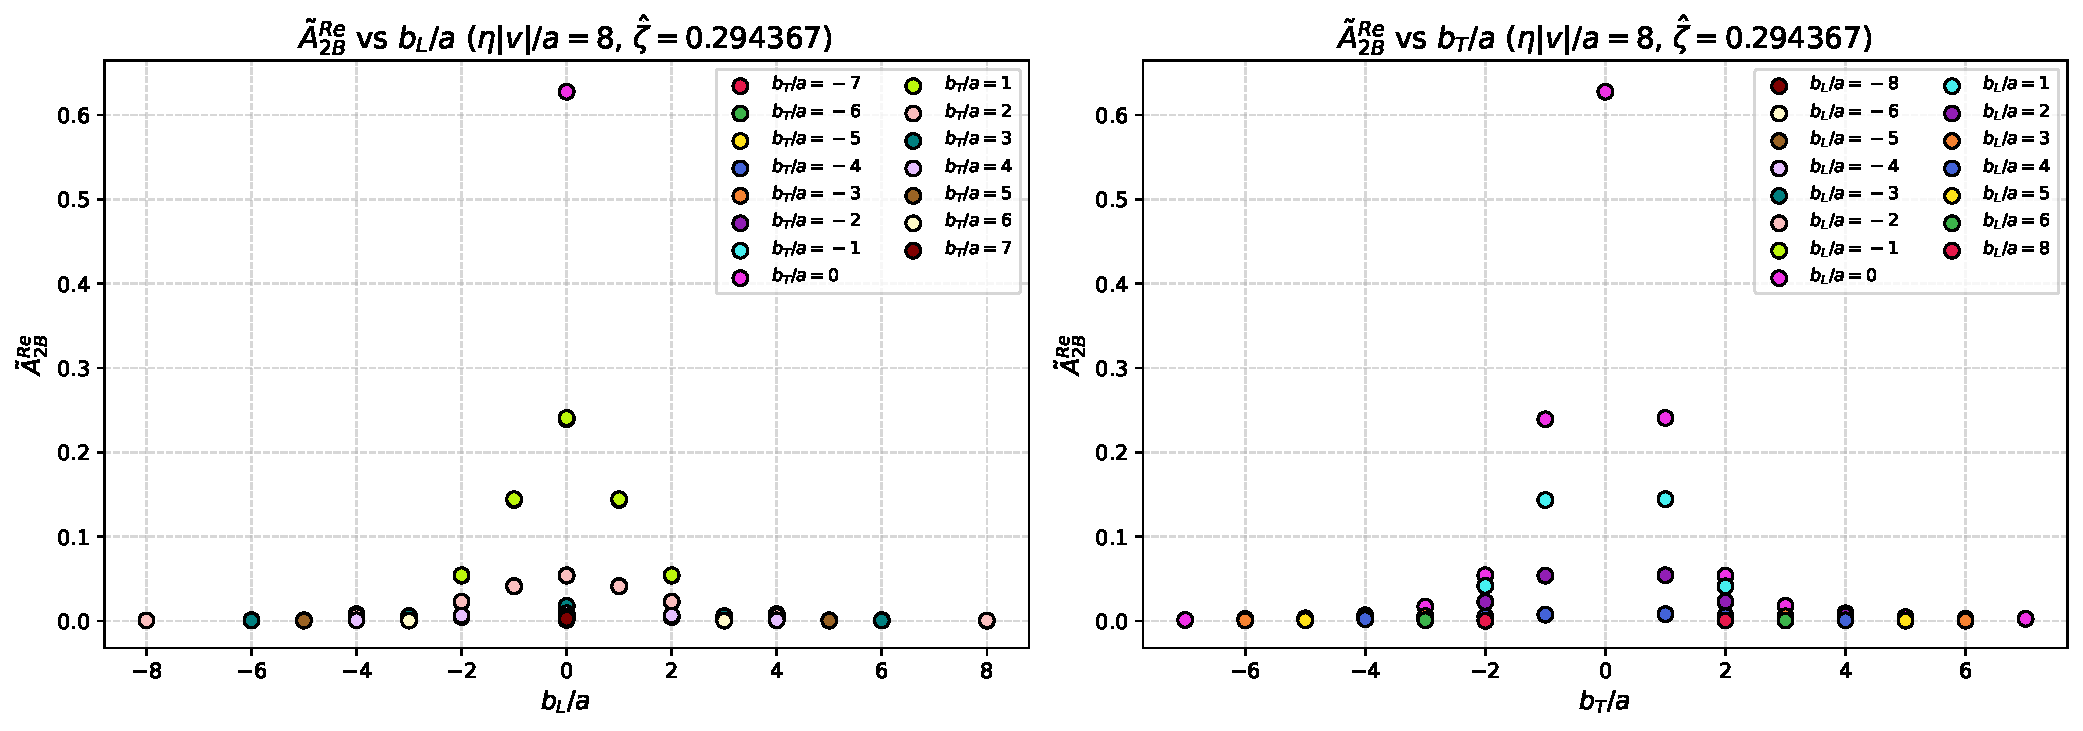
\includegraphics[width=0.98\linewidth,height=0.73\textheight,keepaspectratio]{ReA2B_eta8_PL-2_2D.pdf}\\[1mm]
{\small $\zetahat=0.294367$; $(b_L,b_T)$; $\eta|v|/a=8$ slices}
\figsrc{Thesis, Ch. 5: raw amplitude profiles; complete original panels.}
\end{frame}

\begin{frame}{$\tAmp_{2B}^{\mathrm{Re}}$ at $P_L=-2$: invariant coordinates}
\centering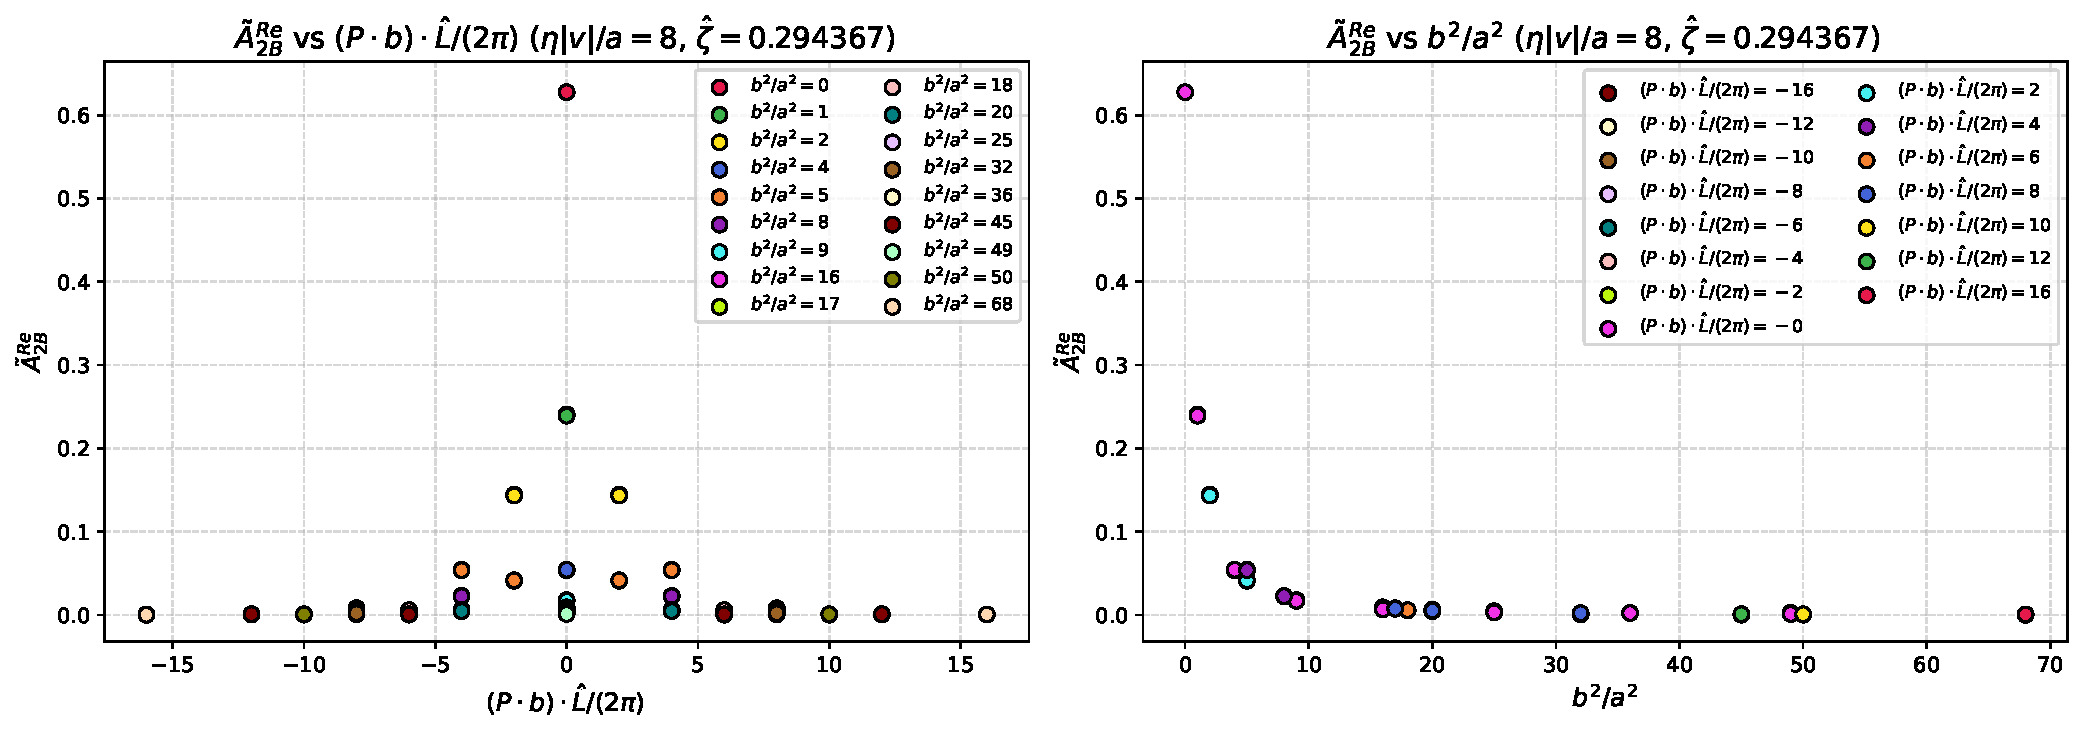
\includegraphics[width=0.98\linewidth,height=0.73\textheight,keepaspectratio]{ReA2B_Pb_bsq_eta8_PL-2_2D.pdf}\\[1mm]
{\small $\zetahat=0.294367$; $(\nu,s)$; $\eta|v|/a=8$ slices}
\figsrc{Thesis, Ch. 5: raw amplitude profiles; complete original panels.}
\end{frame}

\begin{frame}{$\tAmp_{2B}^{\mathrm{Im}}$ at $P_L=-2$: lattice coordinates}
\centering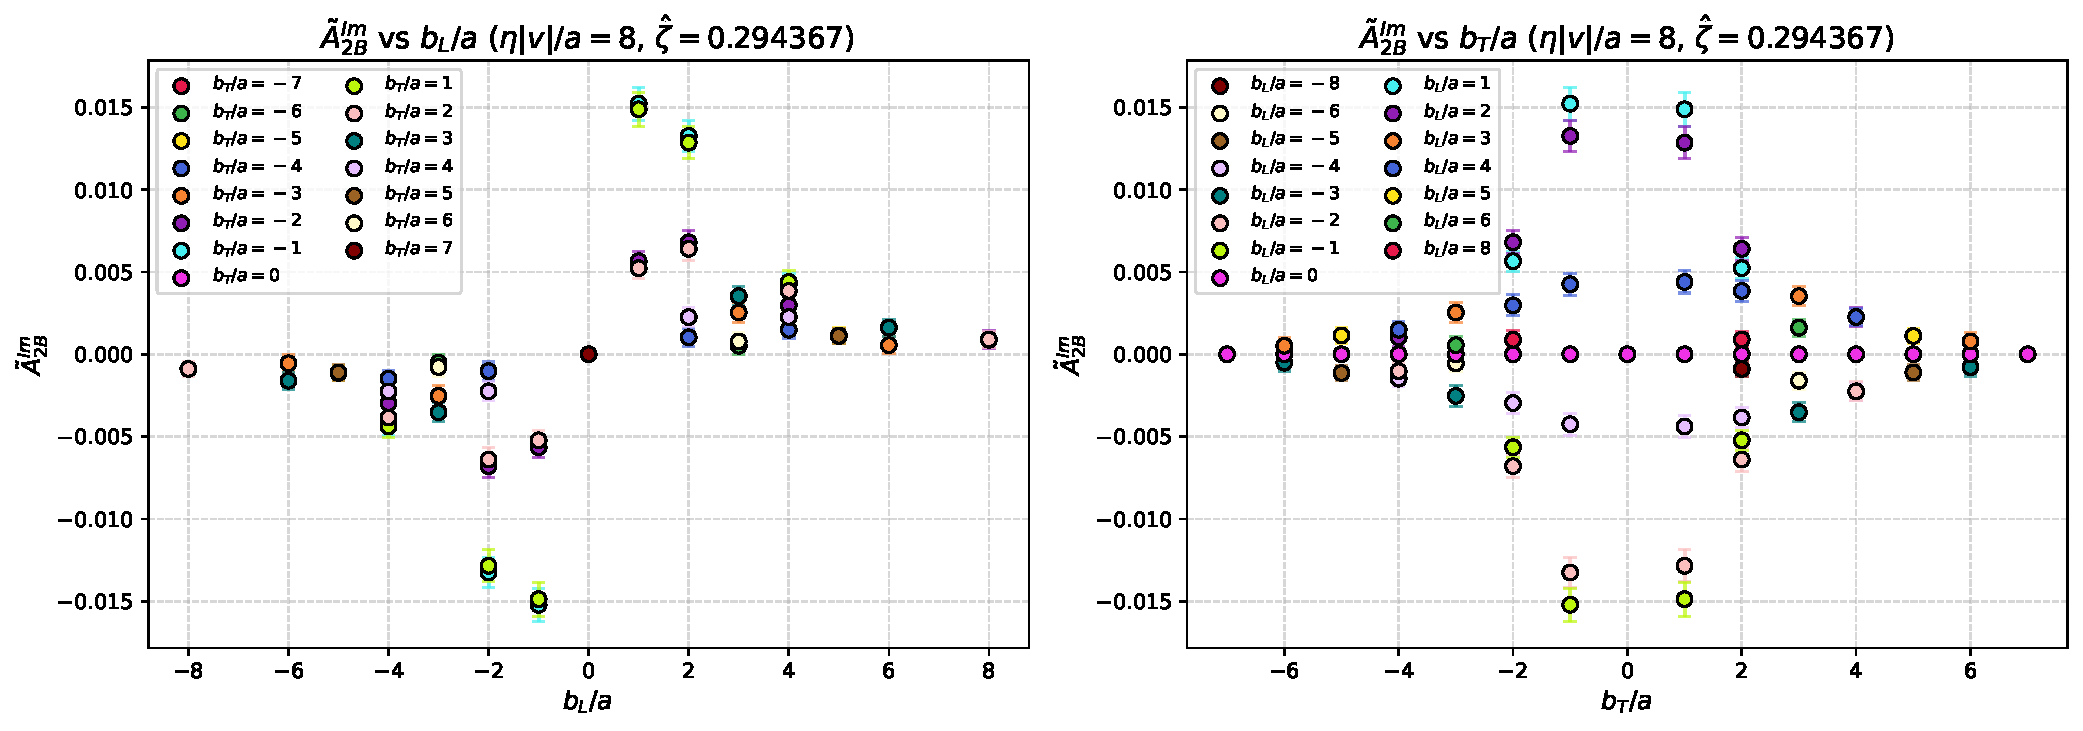
\includegraphics[width=0.98\linewidth,height=0.73\textheight,keepaspectratio]{ImA2B_eta8_PL-2_2D.pdf}\\[1mm]
{\small $\zetahat=0.294367$; $(b_L,b_T)$; $\eta|v|/a=8$ slices}
\figsrc{Thesis, Ch. 5: raw amplitude profiles; complete original panels.}
\end{frame}

\begin{frame}{$\tAmp_{2B}^{\mathrm{Im}}$ at $P_L=-2$: invariant coordinates}
\centering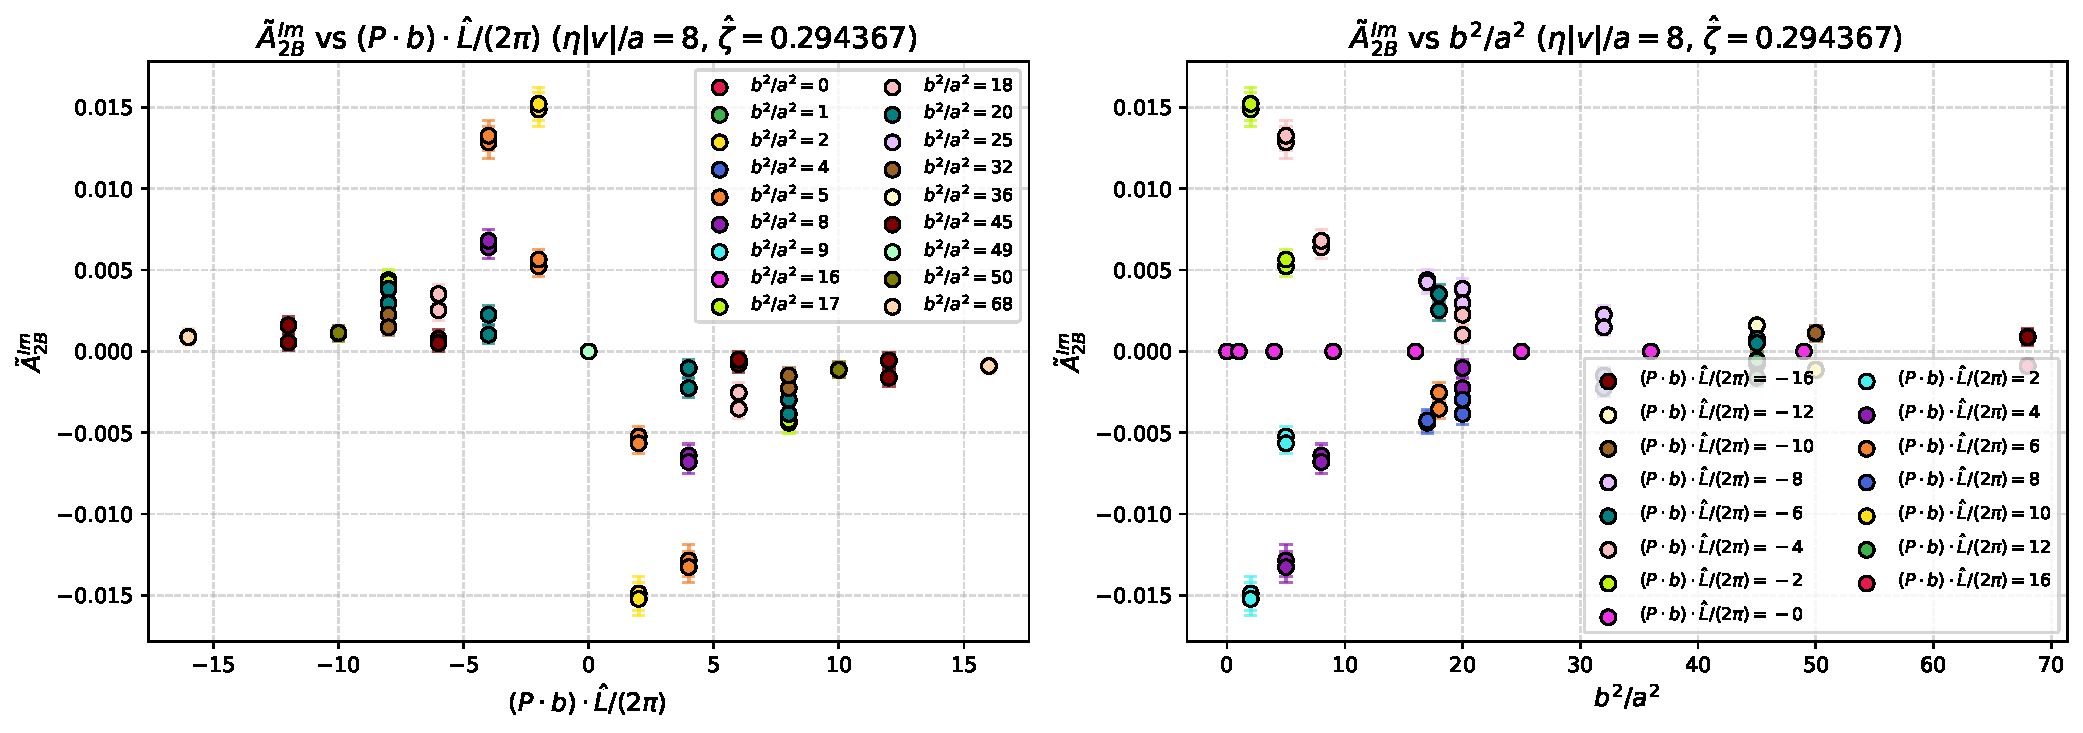
\includegraphics[width=0.98\linewidth,height=0.73\textheight,keepaspectratio]{ImA2B_Pb_bsq_eta8_PL-2_2D.pdf}\\[1mm]
{\small $\zetahat=0.294367$; $(\nu,s)$; $\eta|v|/a=8$ slices}
\figsrc{Thesis, Ch. 5: raw amplitude profiles; complete original panels.}
\end{frame}

\begin{frame}{$\tAmp_{12B}^{\mathrm{Re}}$ at $P_L=-2$: lattice coordinates}
\centering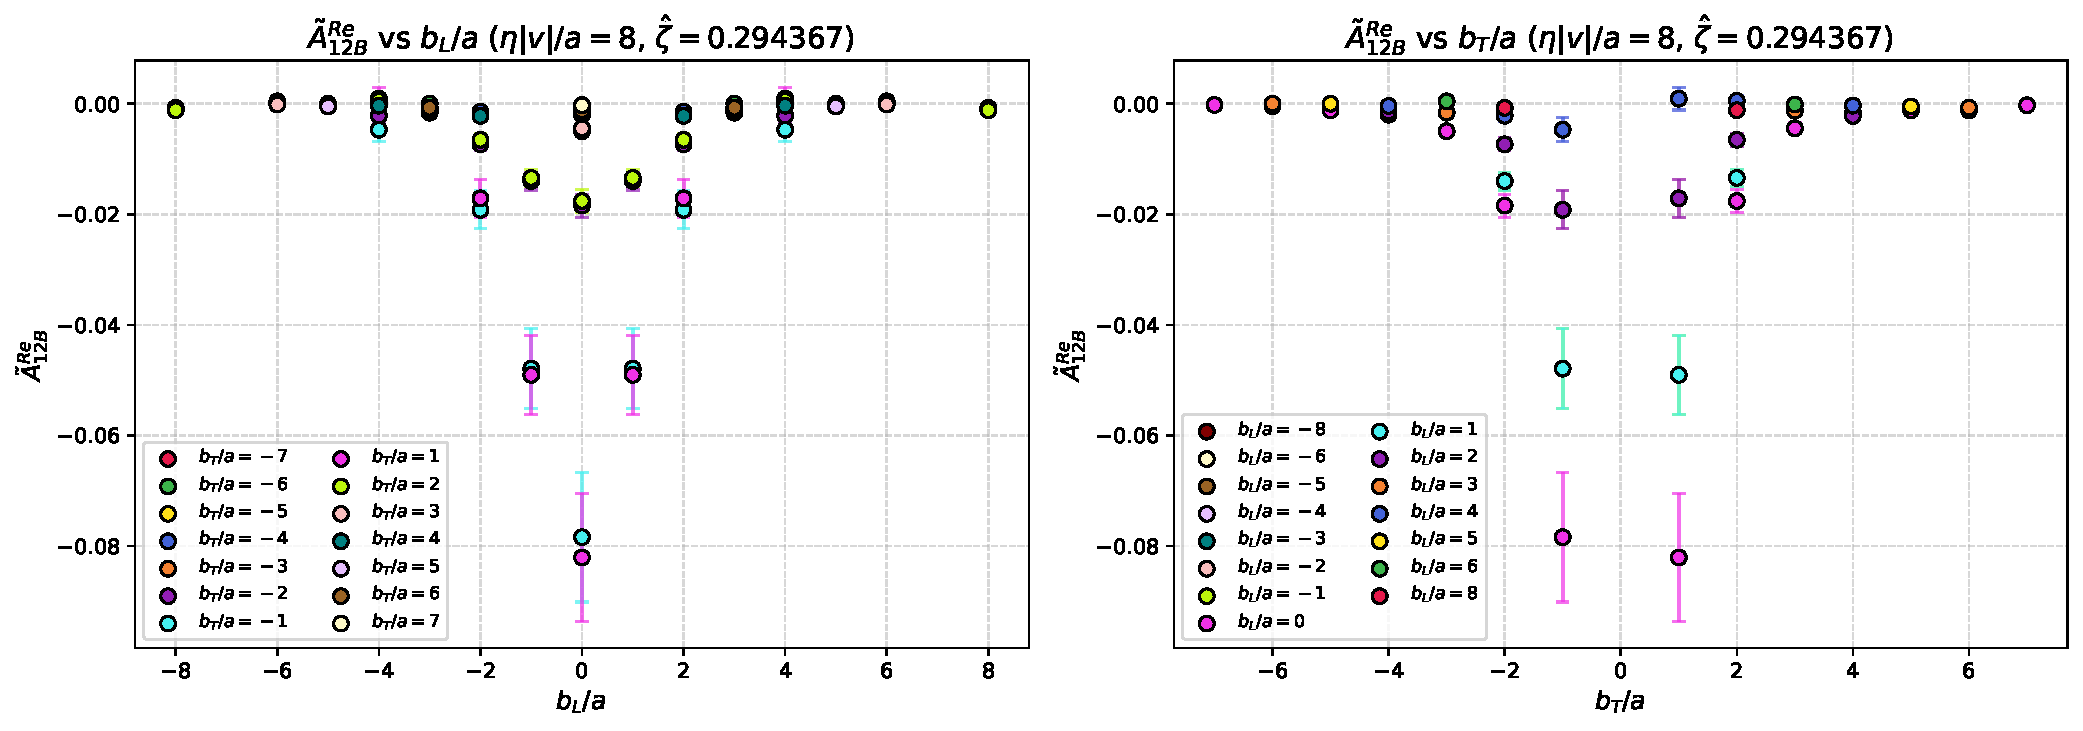
\includegraphics[width=0.98\linewidth,height=0.73\textheight,keepaspectratio]{ReA12B_eta8_PL-2_2D.pdf}\\[1mm]
{\small $\zetahat=0.294367$; $(b_L,b_T)$; $\eta|v|/a=8$ slices}
\figsrc{Thesis, Ch. 5: raw amplitude profiles; complete original panels.}
\end{frame}

\begin{frame}{$\tAmp_{12B}^{\mathrm{Re}}$ at $P_L=-2$: invariant coordinates}
\centering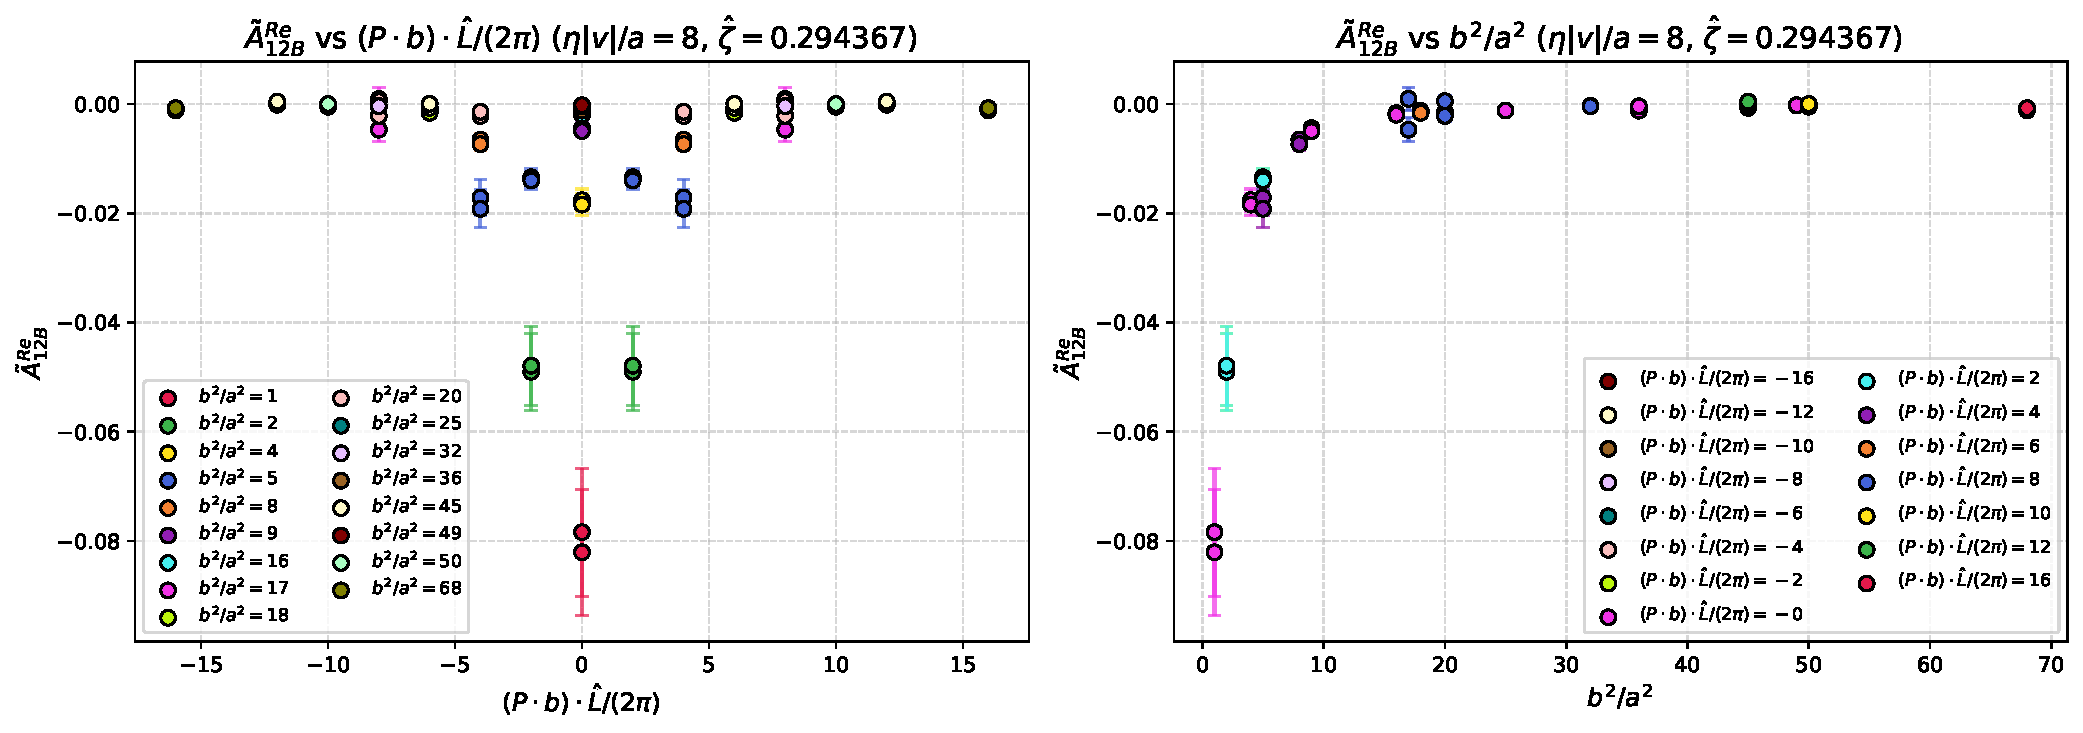
\includegraphics[width=0.98\linewidth,height=0.73\textheight,keepaspectratio]{ReA12B_Pb_bsq_eta8_PL-2_2D.pdf}\\[1mm]
{\small $\zetahat=0.294367$; $(\nu,s)$; $\eta|v|/a=8$ slices}
\figsrc{Thesis, Ch. 5: raw amplitude profiles; complete original panels.}
\end{frame}

\begin{frame}{$\tAmp_{12B}^{\mathrm{Im}}$ at $P_L=-2$: lattice coordinates}
\centering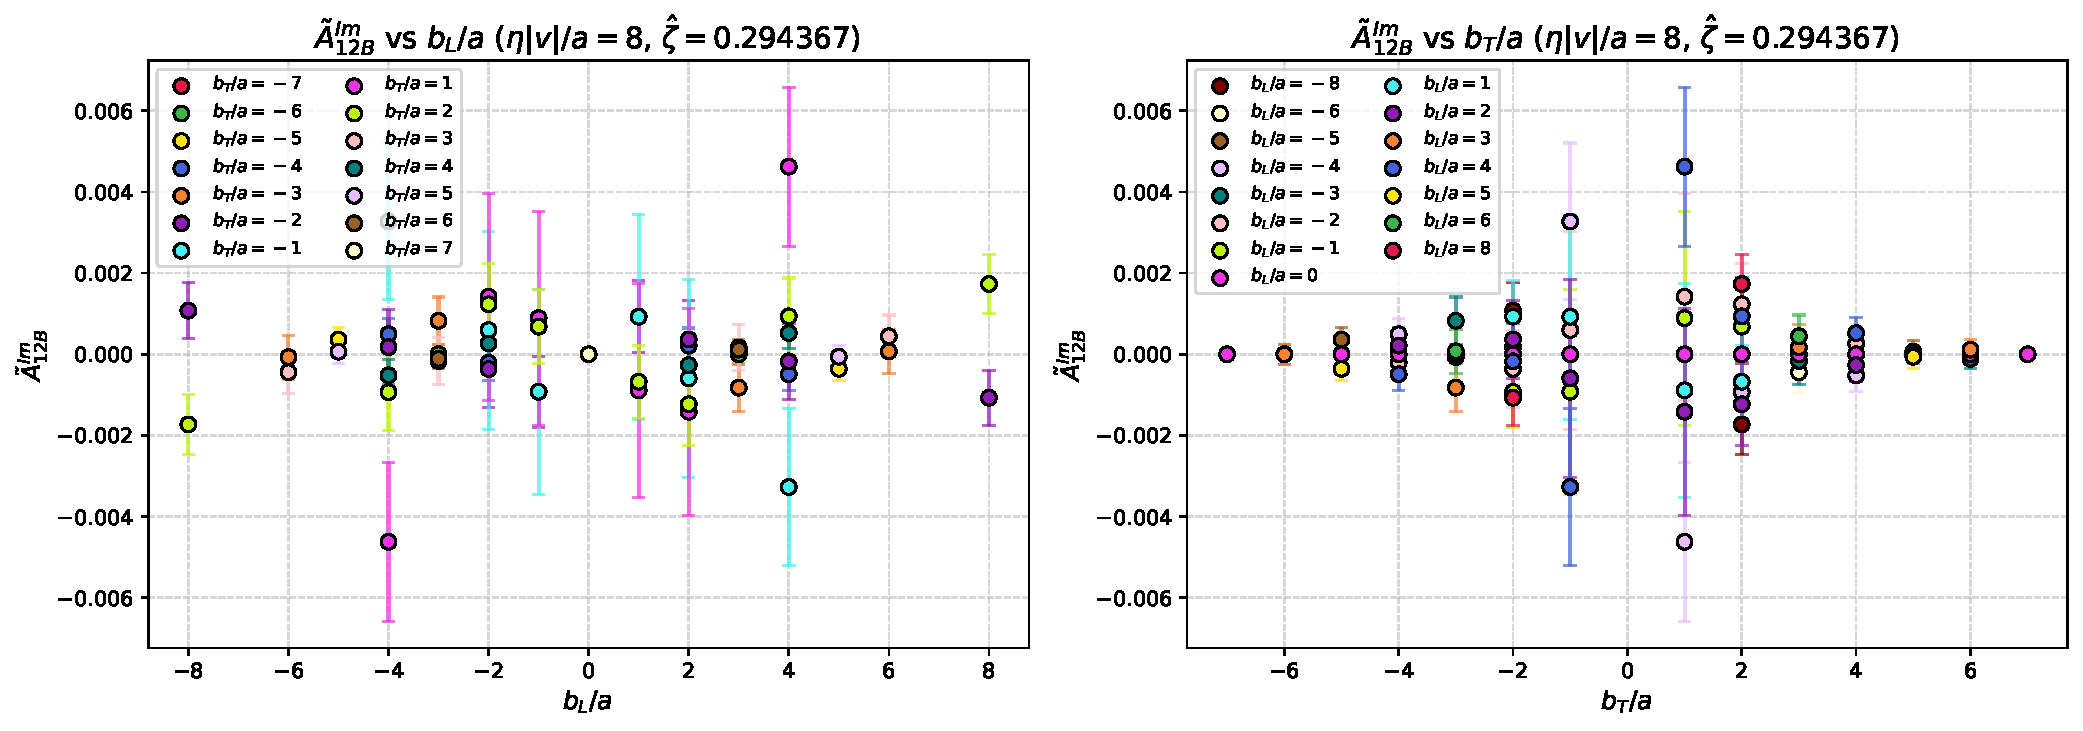
\includegraphics[width=0.98\linewidth,height=0.73\textheight,keepaspectratio]{ImA12B_eta8_PL-2_2D.pdf}\\[1mm]
{\small $\zetahat=0.294367$; $(b_L,b_T)$; $\eta|v|/a=8$ slices}
\figsrc{Thesis, Ch. 5: raw amplitude profiles; complete original panels.}
\end{frame}

\begin{frame}{$\tAmp_{12B}^{\mathrm{Im}}$ at $P_L=-2$: invariant coordinates}
\centering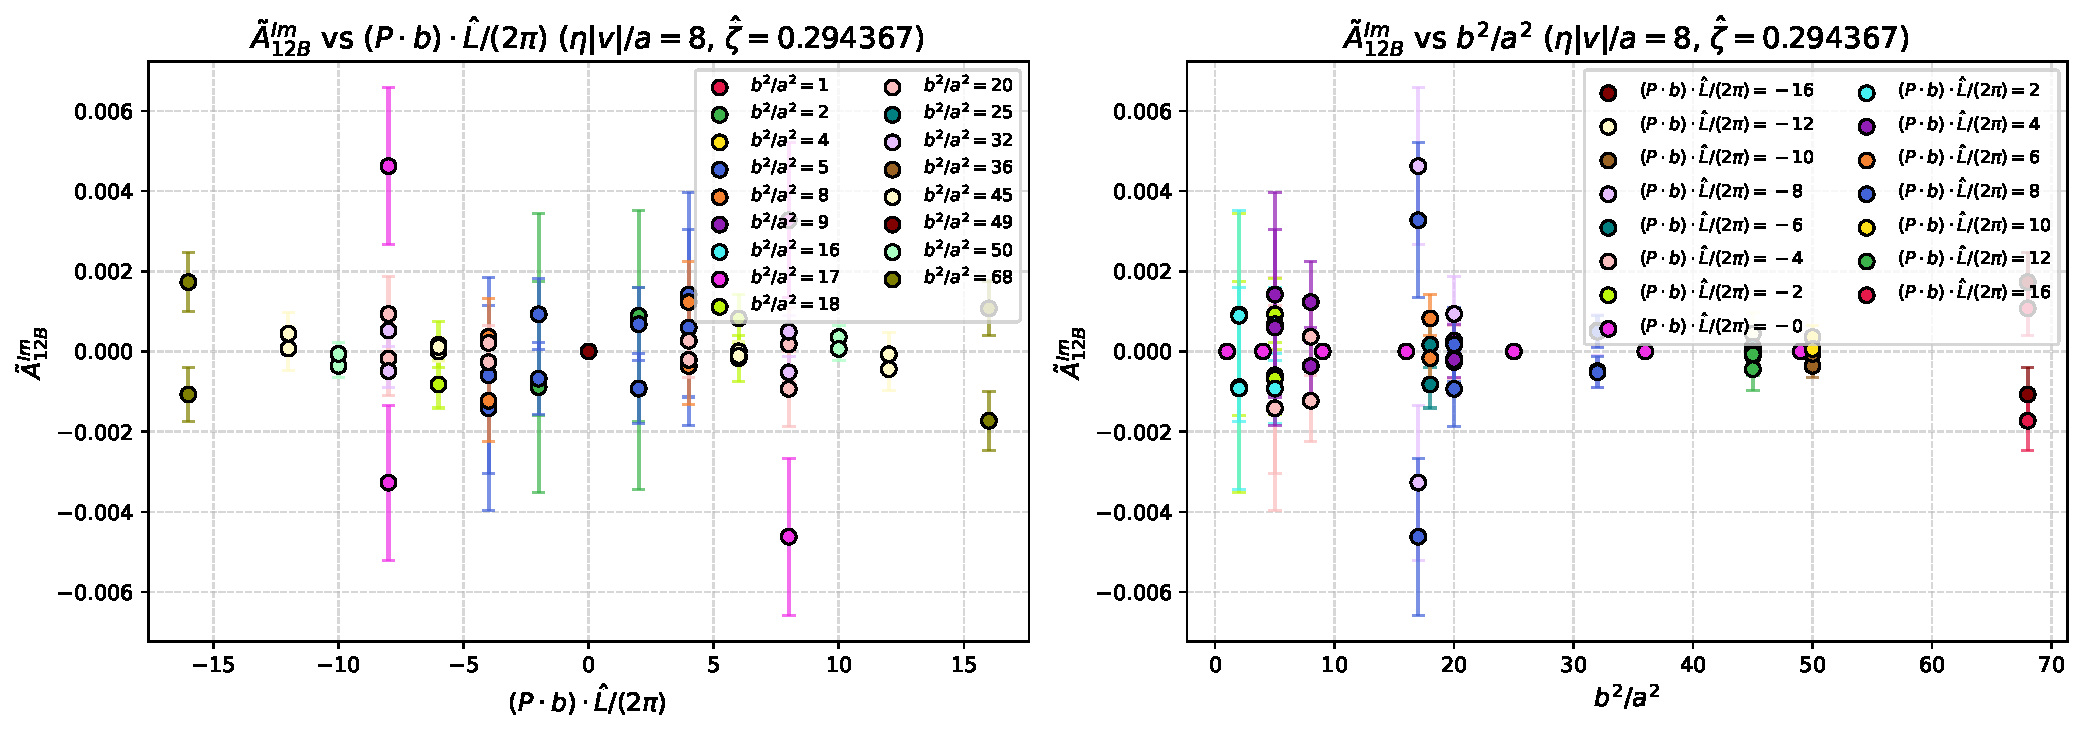
\includegraphics[width=0.98\linewidth,height=0.73\textheight,keepaspectratio]{ImA12B_Pb_bsq_eta8_PL-2_2D.pdf}\\[1mm]
{\small $\zetahat=0.294367$; $(\nu,s)$; $\eta|v|/a=8$ slices}
\figsrc{Thesis, Ch. 5: raw amplitude profiles; complete original panels.}
\end{frame}

\begin{frame}{$\tAmp_{2B}^{\mathrm{Re}}$ at $P_L=-3$: lattice coordinates}
\centering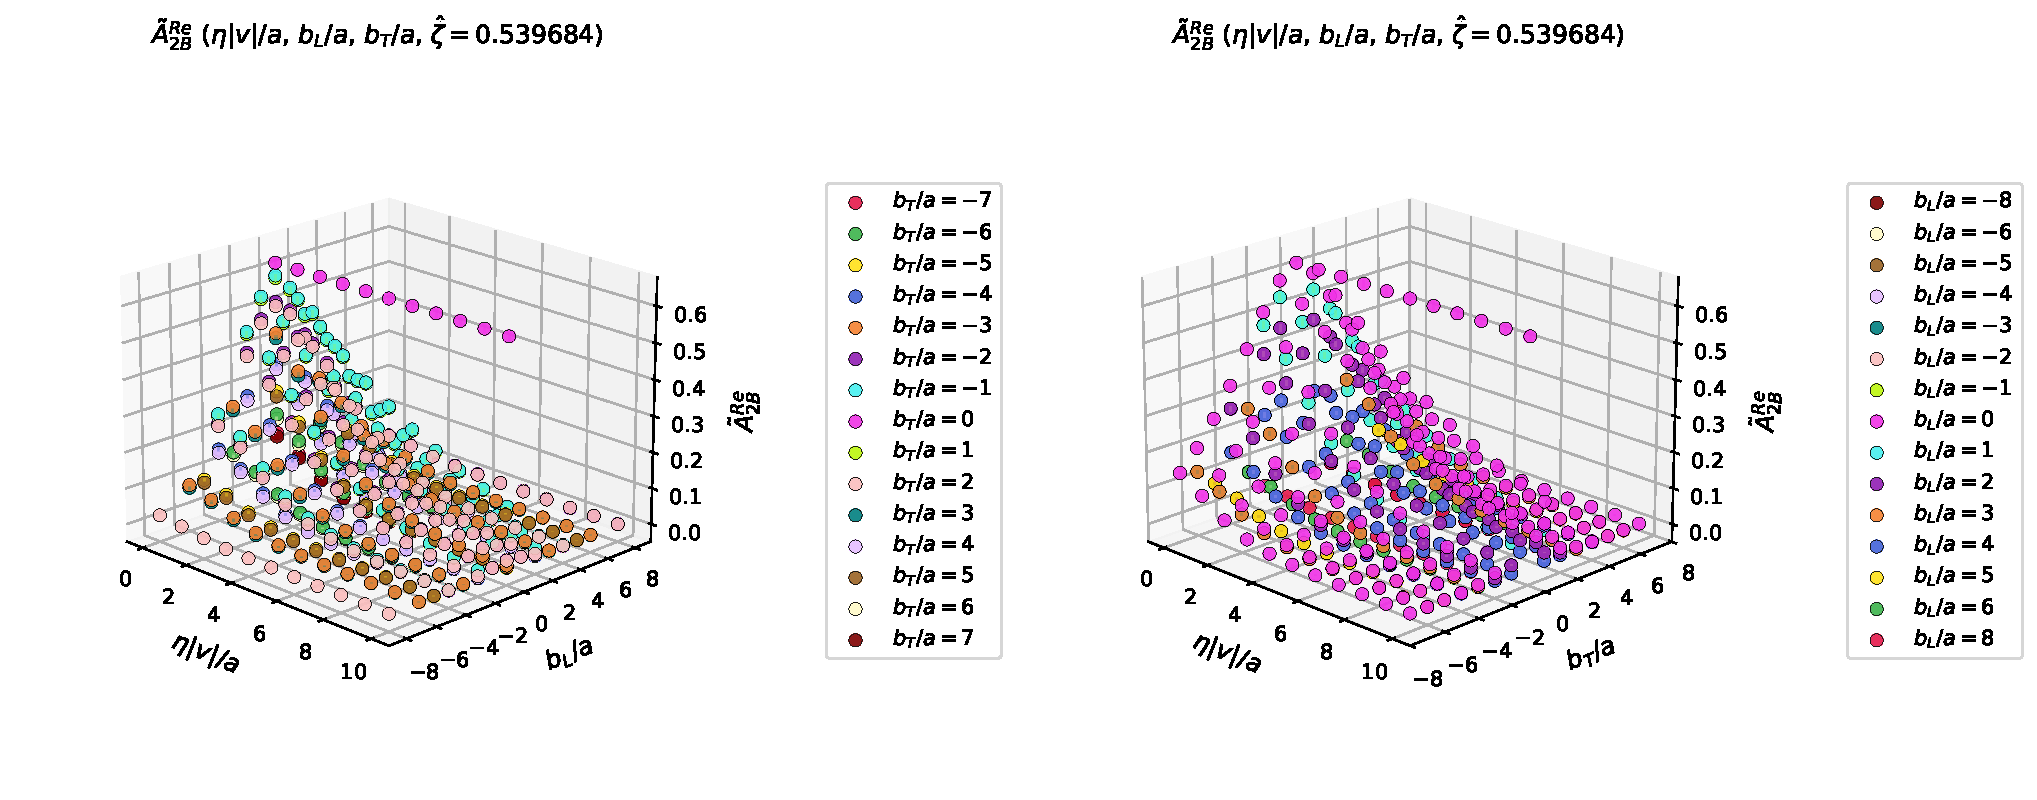
\includegraphics[width=0.98\linewidth,height=0.73\textheight,keepaspectratio]{ReA2B_PL-3_3D.pdf}\\[1mm]
{\small $\zetahat=0.539684$; $(b_L,b_T)$; staple-length dependence}
\figsrc{Thesis, Ch. 5: raw amplitude profiles; complete original panels.}
\end{frame}

\begin{frame}{$\tAmp_{2B}^{\mathrm{Re}}$ at $P_L=-3$: invariant coordinates}
\centering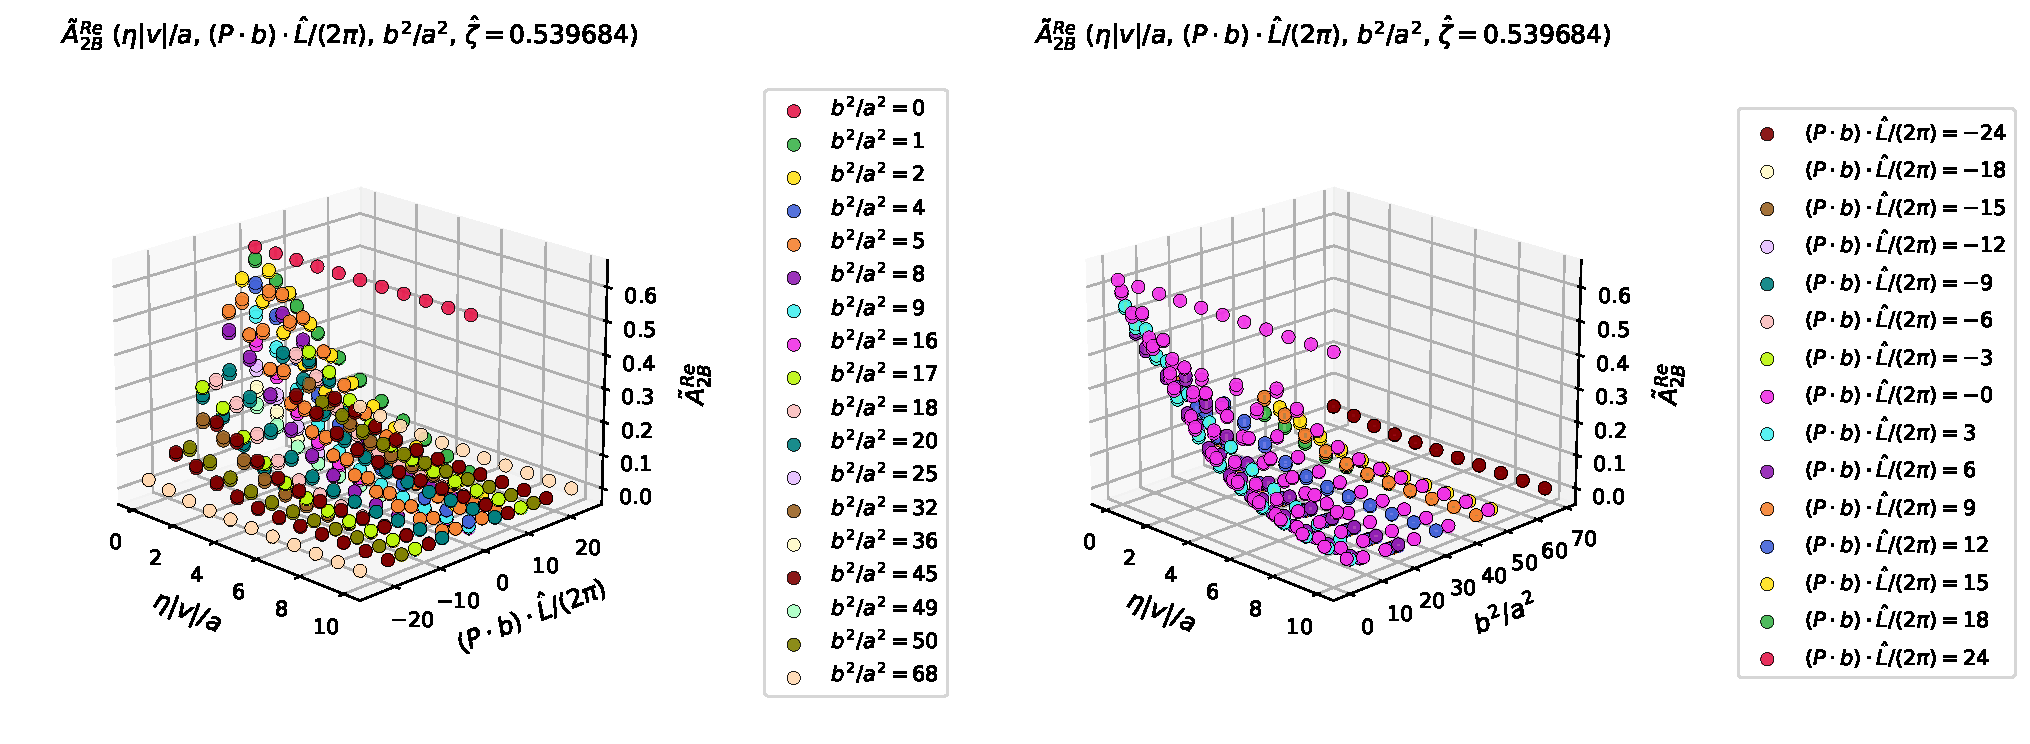
\includegraphics[width=0.98\linewidth,height=0.73\textheight,keepaspectratio]{ReA2B_Pb_bsq_PL-3_3D.pdf}\\[1mm]
{\small $\zetahat=0.539684$; $(\nu,s)$; staple-length dependence}
\figsrc{Thesis, Ch. 5: raw amplitude profiles; complete original panels.}
\end{frame}

\begin{frame}{$\tAmp_{2B}^{\mathrm{Im}}$ at $P_L=-3$: lattice coordinates}
\centering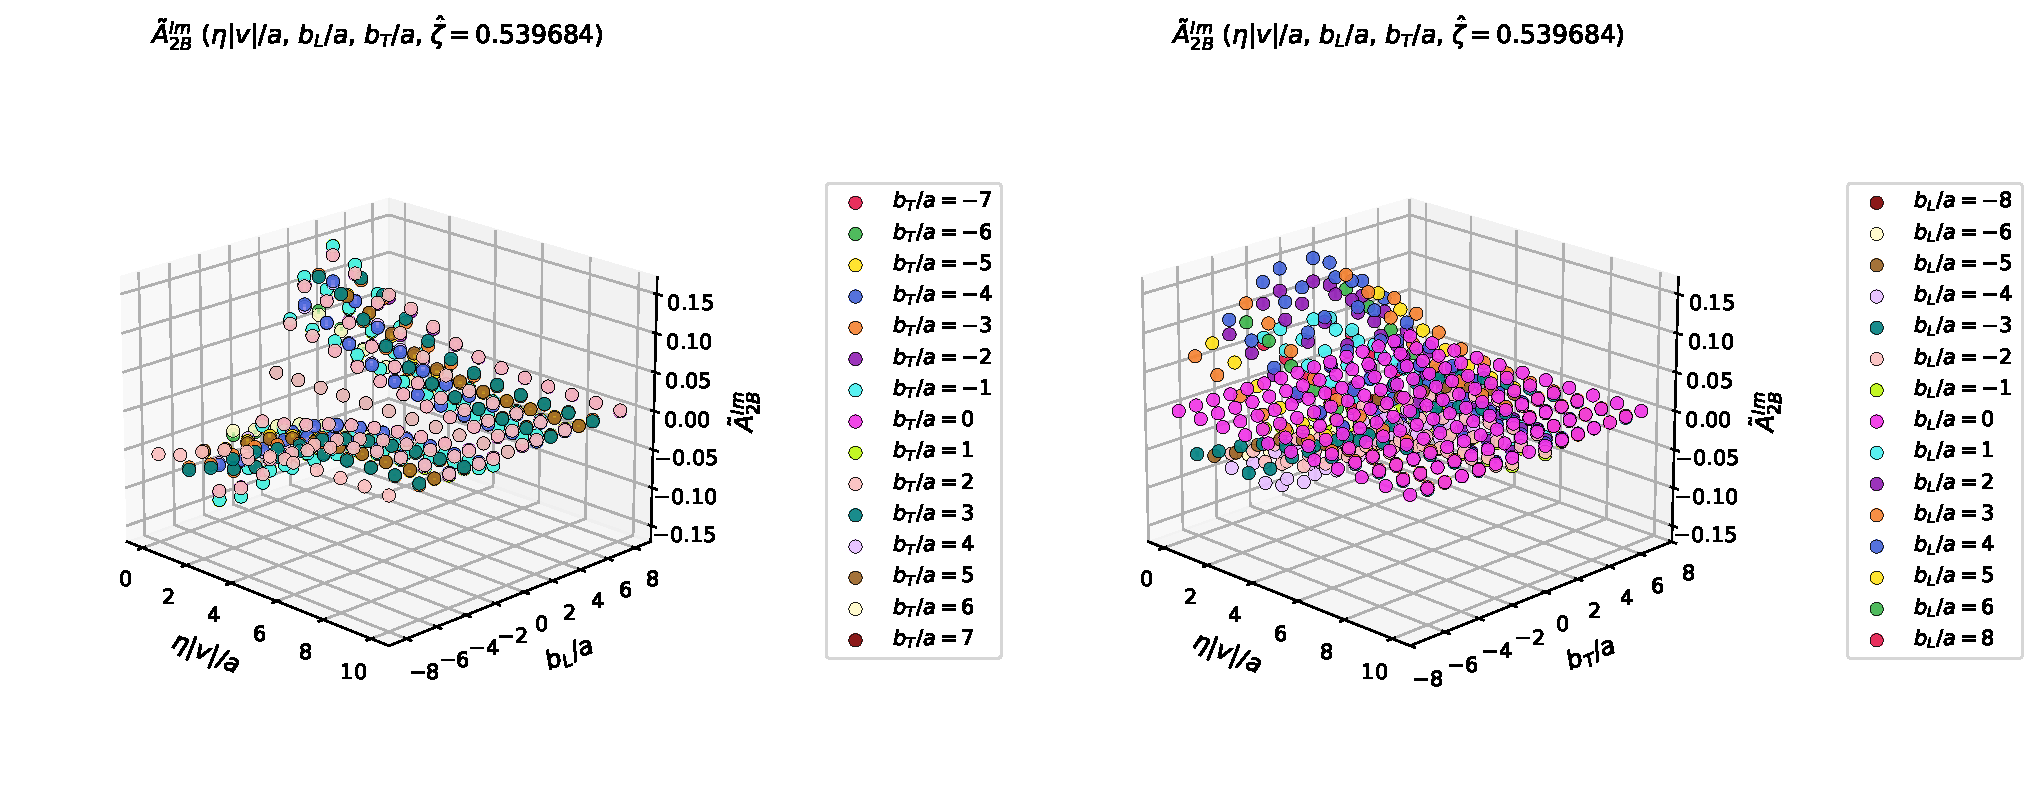
\includegraphics[width=0.98\linewidth,height=0.73\textheight,keepaspectratio]{ImA2B_PL-3_3D.pdf}\\[1mm]
{\small $\zetahat=0.539684$; $(b_L,b_T)$; staple-length dependence}
\figsrc{Thesis, Ch. 5: raw amplitude profiles; complete original panels.}
\end{frame}

\begin{frame}{$\tAmp_{2B}^{\mathrm{Im}}$ at $P_L=-3$: invariant coordinates}
\centering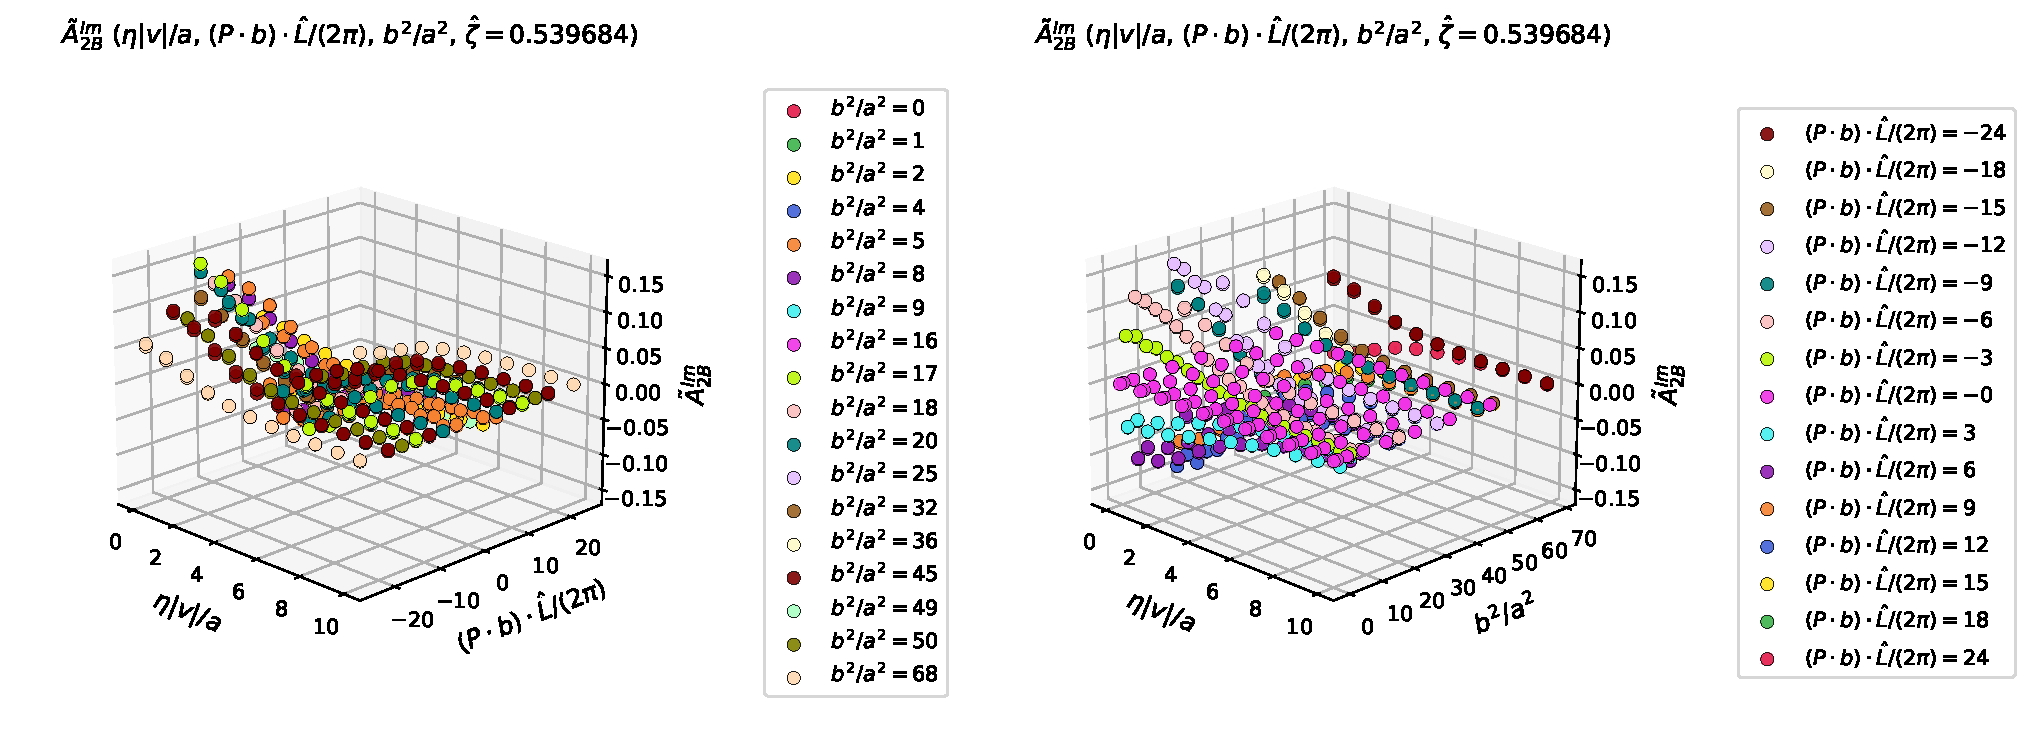
\includegraphics[width=0.98\linewidth,height=0.73\textheight,keepaspectratio]{ImA2B_Pb_bsq_PL-3_3D.pdf}\\[1mm]
{\small $\zetahat=0.539684$; $(\nu,s)$; staple-length dependence}
\figsrc{Thesis, Ch. 5: raw amplitude profiles; complete original panels.}
\end{frame}

\begin{frame}{$\tAmp_{12B}^{\mathrm{Re}}$ at $P_L=-3$: lattice coordinates}
\centering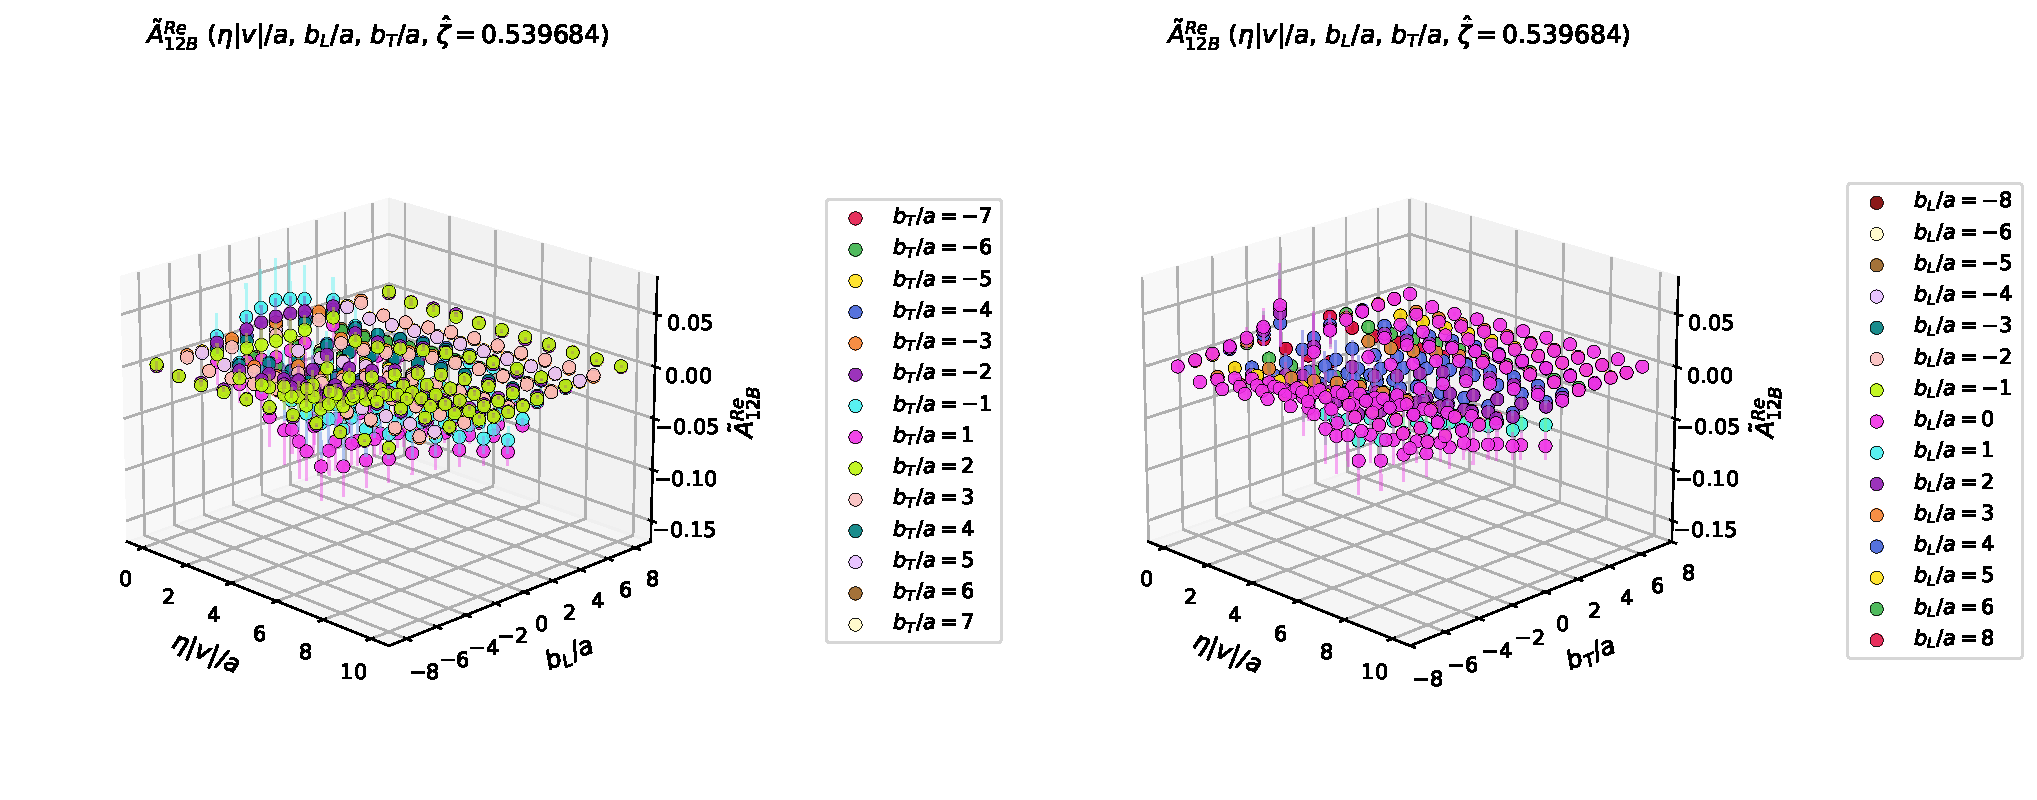
\includegraphics[width=0.98\linewidth,height=0.73\textheight,keepaspectratio]{ReA12B_PL-3_3D.pdf}\\[1mm]
{\small $\zetahat=0.539684$; $(b_L,b_T)$; staple-length dependence}
\figsrc{Thesis, Ch. 5: raw amplitude profiles; complete original panels.}
\end{frame}

\begin{frame}{$\tAmp_{12B}^{\mathrm{Re}}$ at $P_L=-3$: invariant coordinates}
\centering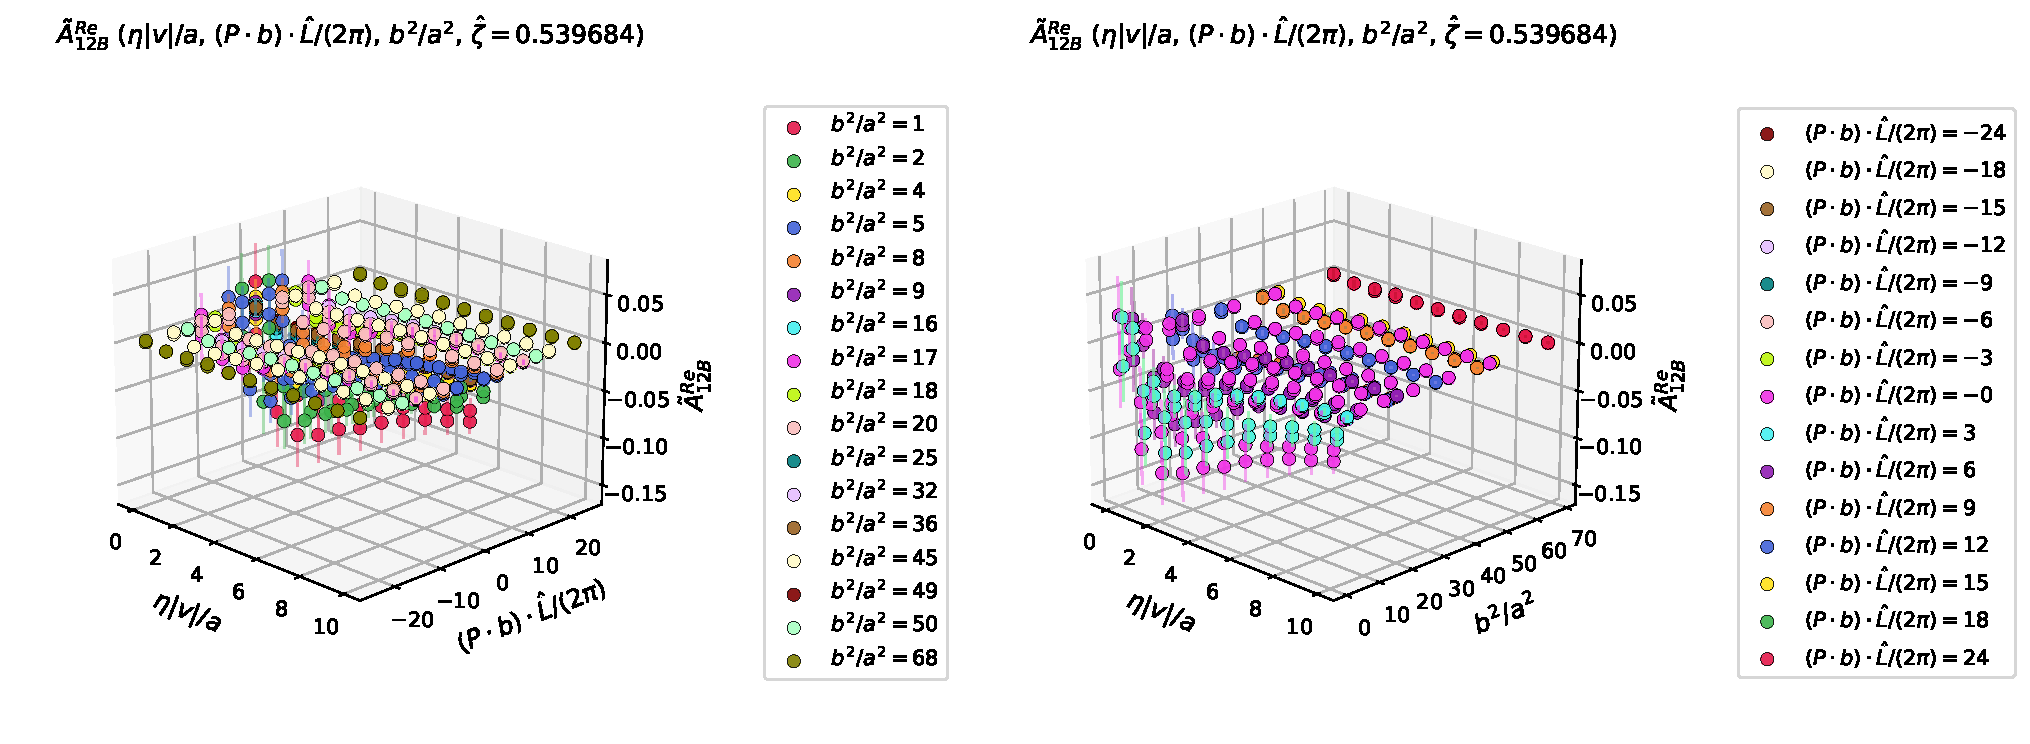
\includegraphics[width=0.98\linewidth,height=0.73\textheight,keepaspectratio]{ReA12B_Pb_bsq_PL-3_3D.pdf}\\[1mm]
{\small $\zetahat=0.539684$; $(\nu,s)$; staple-length dependence}
\figsrc{Thesis, Ch. 5: raw amplitude profiles; complete original panels.}
\end{frame}

\begin{frame}{$\tAmp_{12B}^{\mathrm{Im}}$ at $P_L=-3$: lattice coordinates}
\centering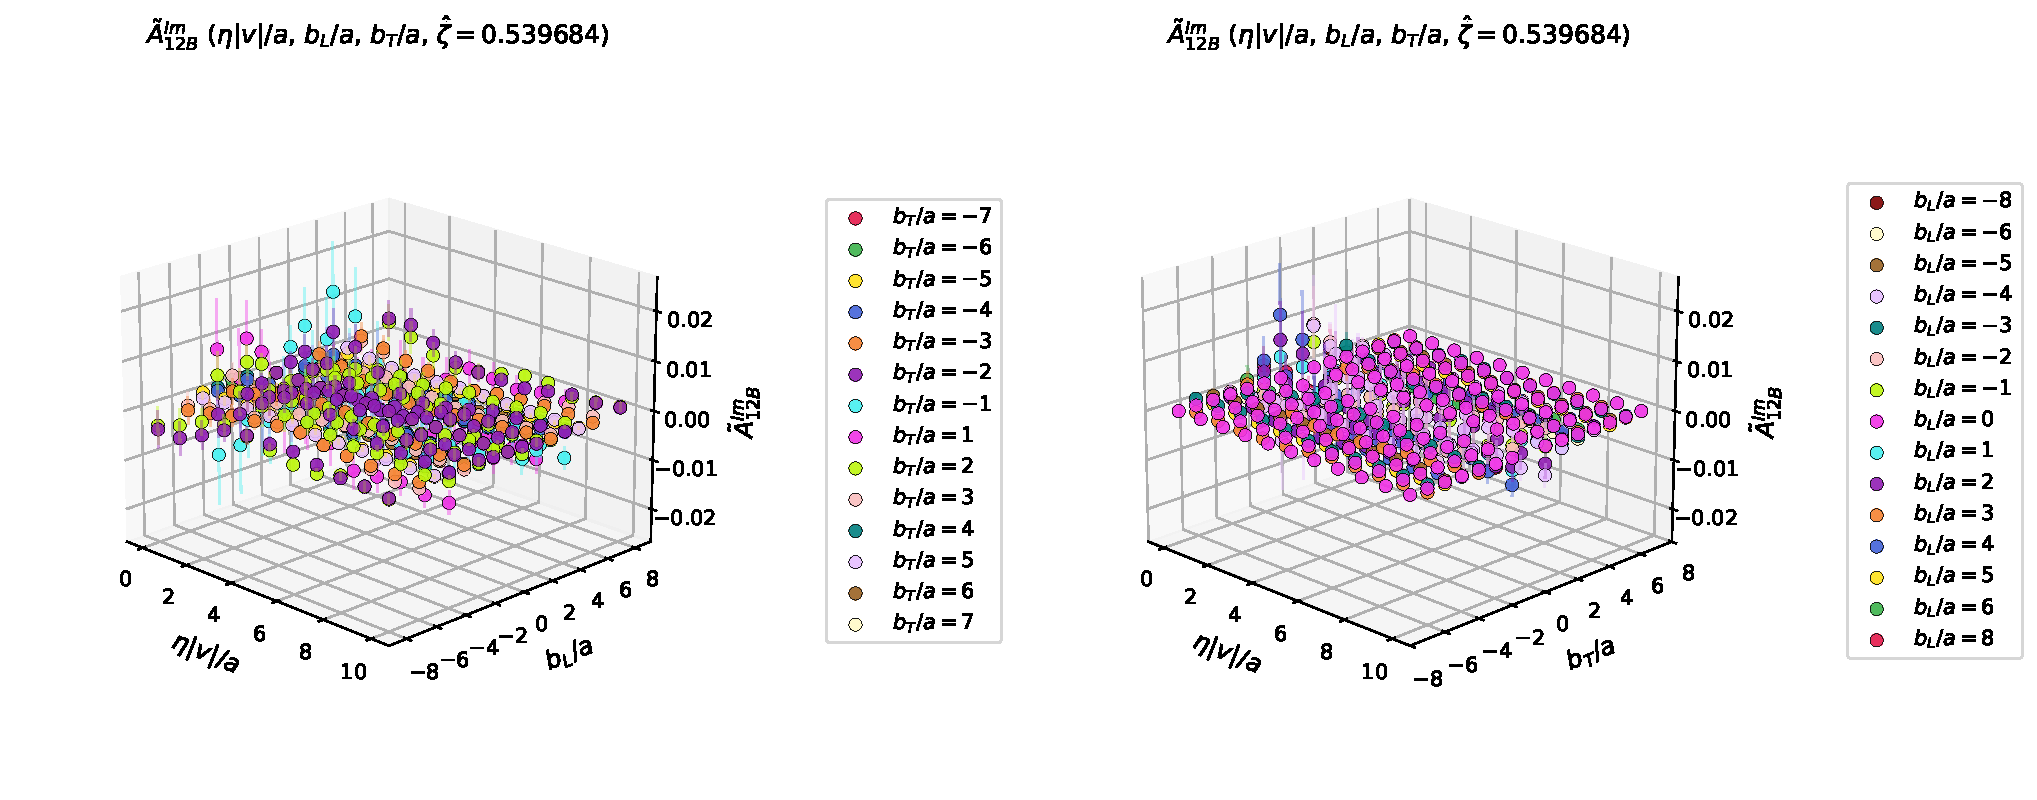
\includegraphics[width=0.98\linewidth,height=0.73\textheight,keepaspectratio]{ImA12B_PL-3_3D.pdf}\\[1mm]
{\small $\zetahat=0.539684$; $(b_L,b_T)$; staple-length dependence}
\figsrc{Thesis, Ch. 5: raw amplitude profiles; complete original panels.}
\end{frame}

\begin{frame}{$\tAmp_{12B}^{\mathrm{Im}}$ at $P_L=-3$: invariant coordinates}
\centering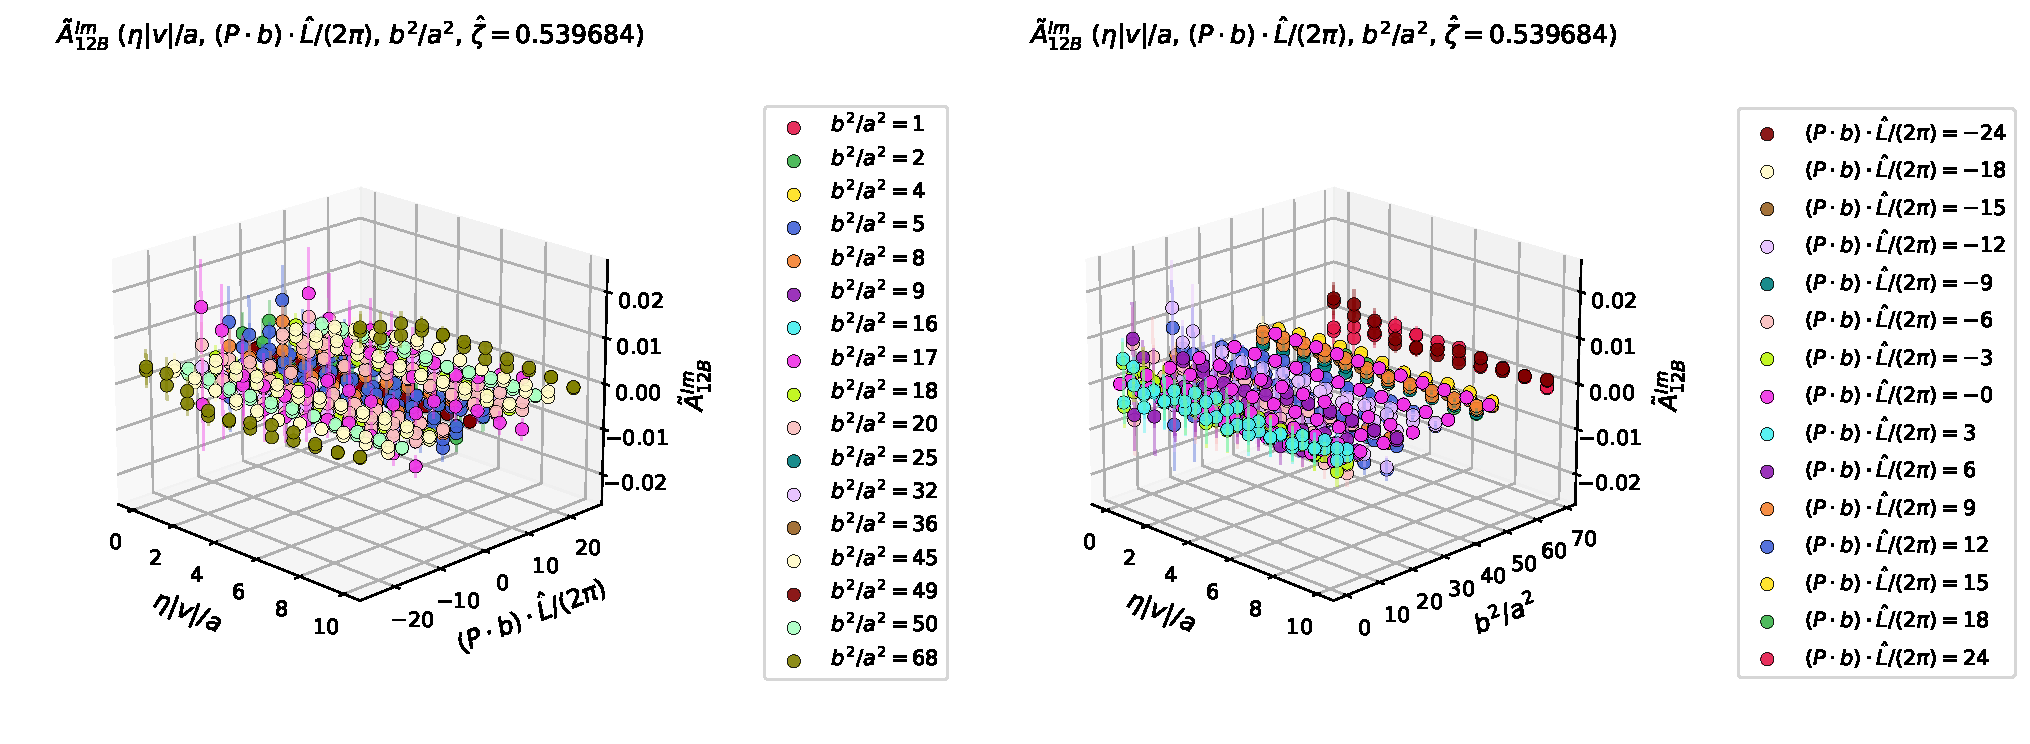
\includegraphics[width=0.98\linewidth,height=0.73\textheight,keepaspectratio]{ImA12B_Pb_bsq_PL-3_3D.pdf}\\[1mm]
{\small $\zetahat=0.539684$; $(\nu,s)$; staple-length dependence}
\figsrc{Thesis, Ch. 5: raw amplitude profiles; complete original panels.}
\end{frame}

\begin{frame}{$\tAmp_{2B}^{\mathrm{Re}}$ at $P_L=-3$: lattice coordinates}
\centering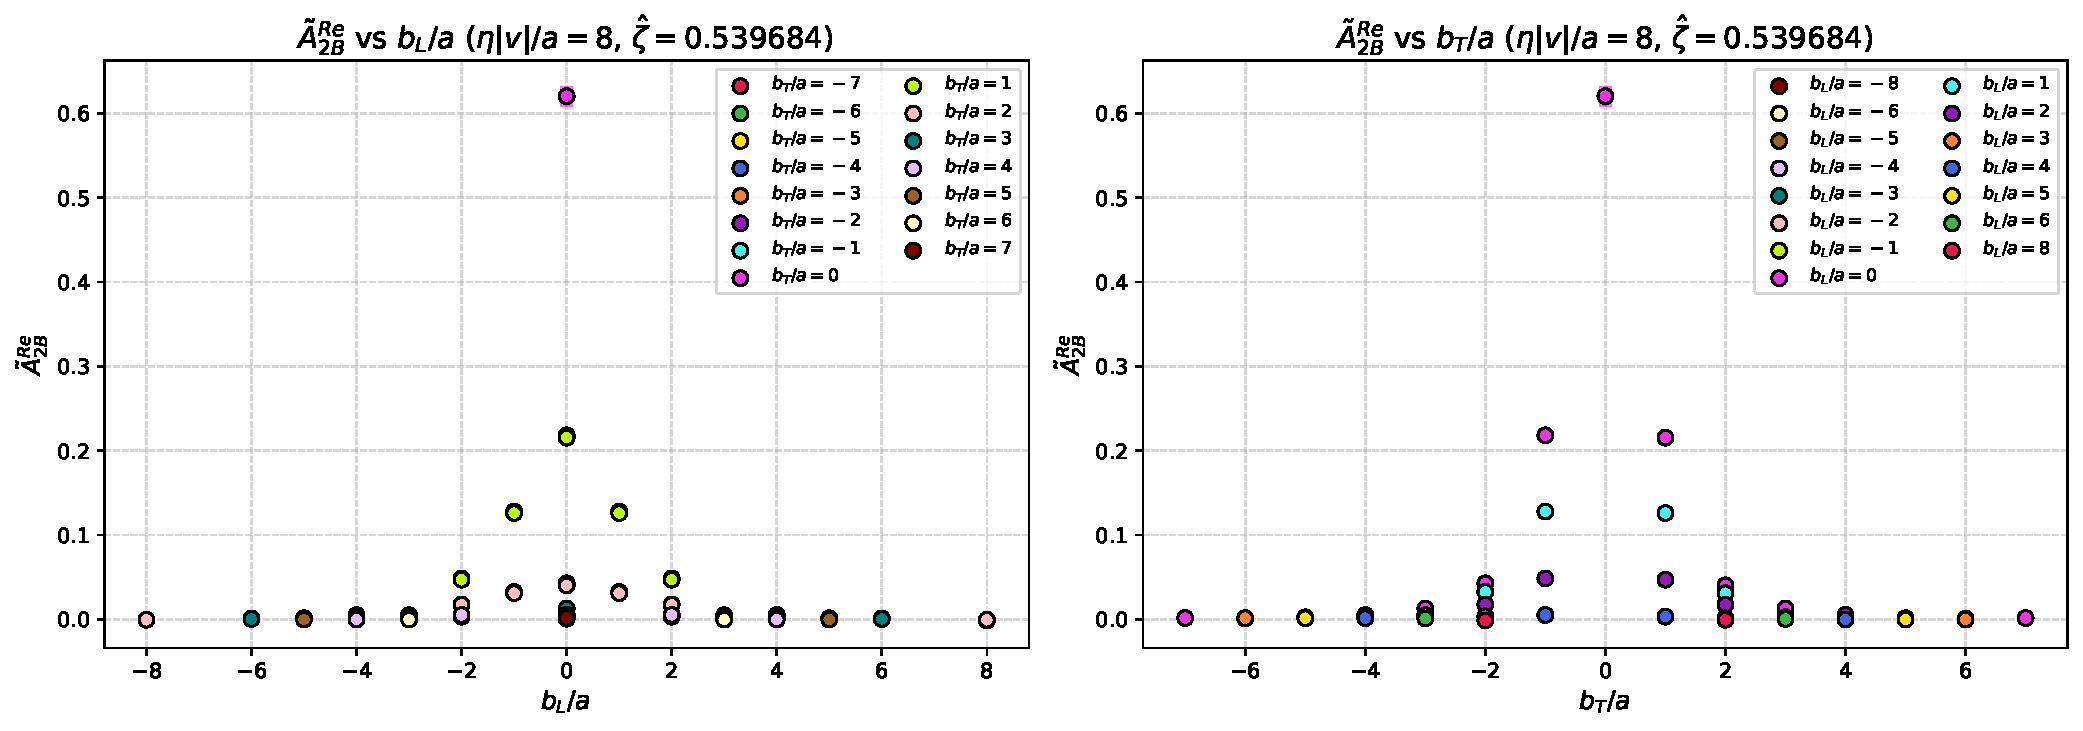
\includegraphics[width=0.98\linewidth,height=0.73\textheight,keepaspectratio]{ReA2B_eta8_PL-3_2D.pdf}\\[1mm]
{\small $\zetahat=0.539684$; $(b_L,b_T)$; $\eta|v|/a=8$ slices}
\figsrc{Thesis, Ch. 5: raw amplitude profiles; complete original panels.}
\end{frame}

\begin{frame}{$\tAmp_{2B}^{\mathrm{Re}}$ at $P_L=-3$: invariant coordinates}
\centering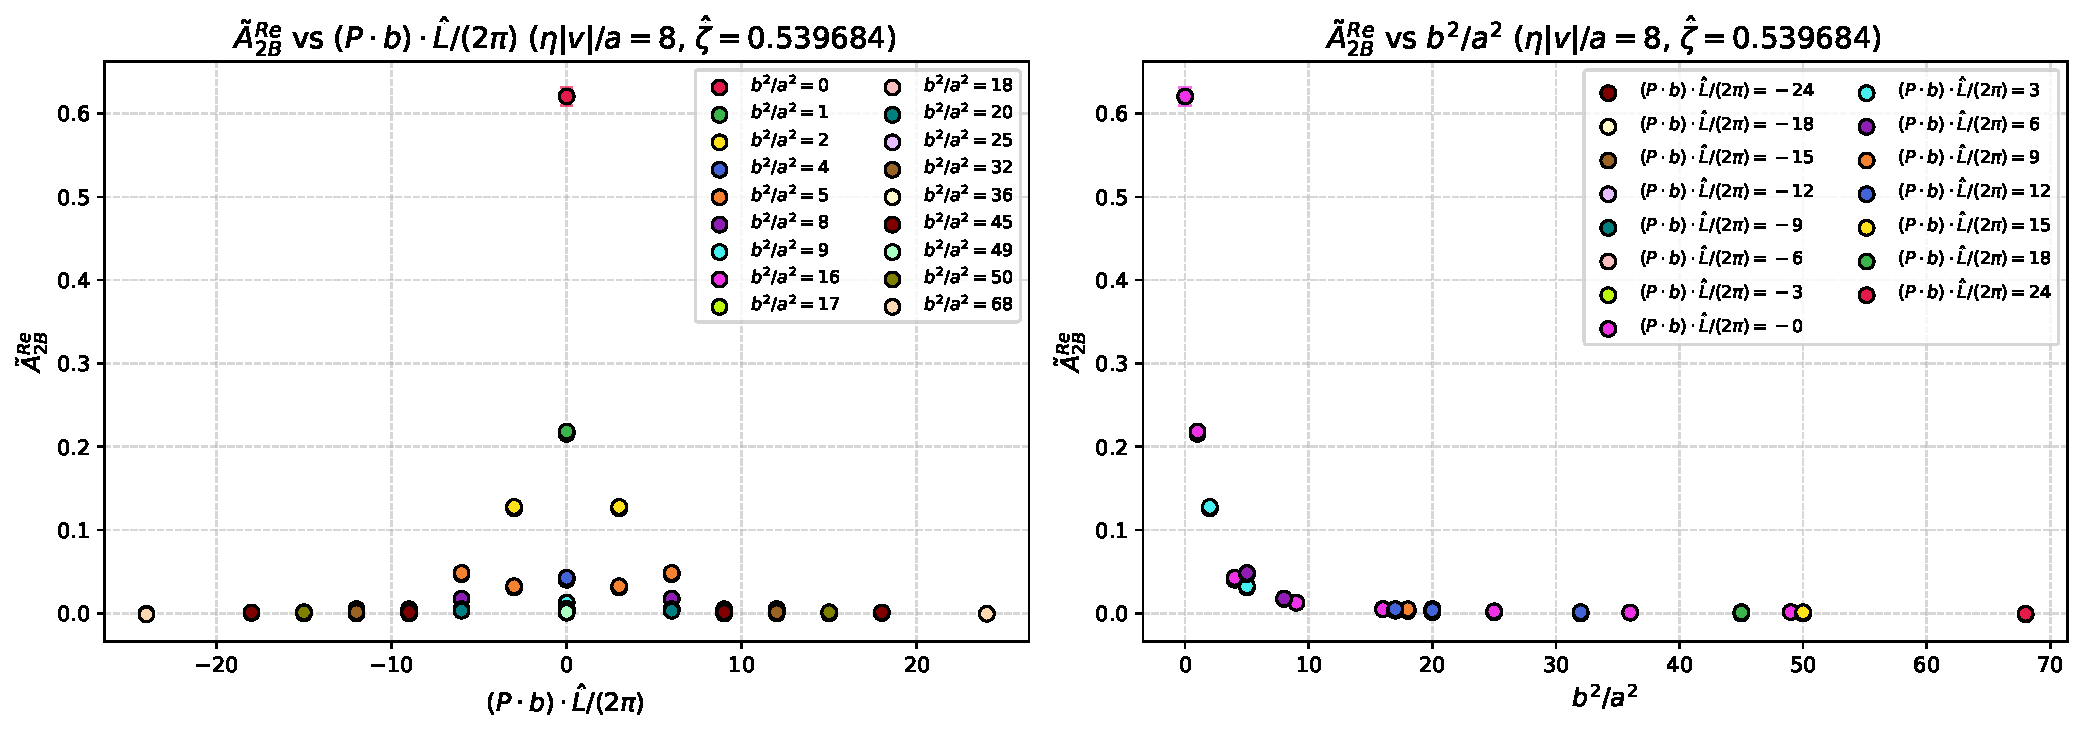
\includegraphics[width=0.98\linewidth,height=0.73\textheight,keepaspectratio]{ReA2B_Pb_bsq_eta8_PL-3_2D.pdf}\\[1mm]
{\small $\zetahat=0.539684$; $(\nu,s)$; $\eta|v|/a=8$ slices}
\figsrc{Thesis, Ch. 5: raw amplitude profiles; complete original panels.}
\end{frame}

\begin{frame}{$\tAmp_{2B}^{\mathrm{Im}}$ at $P_L=-3$: lattice coordinates}
\centering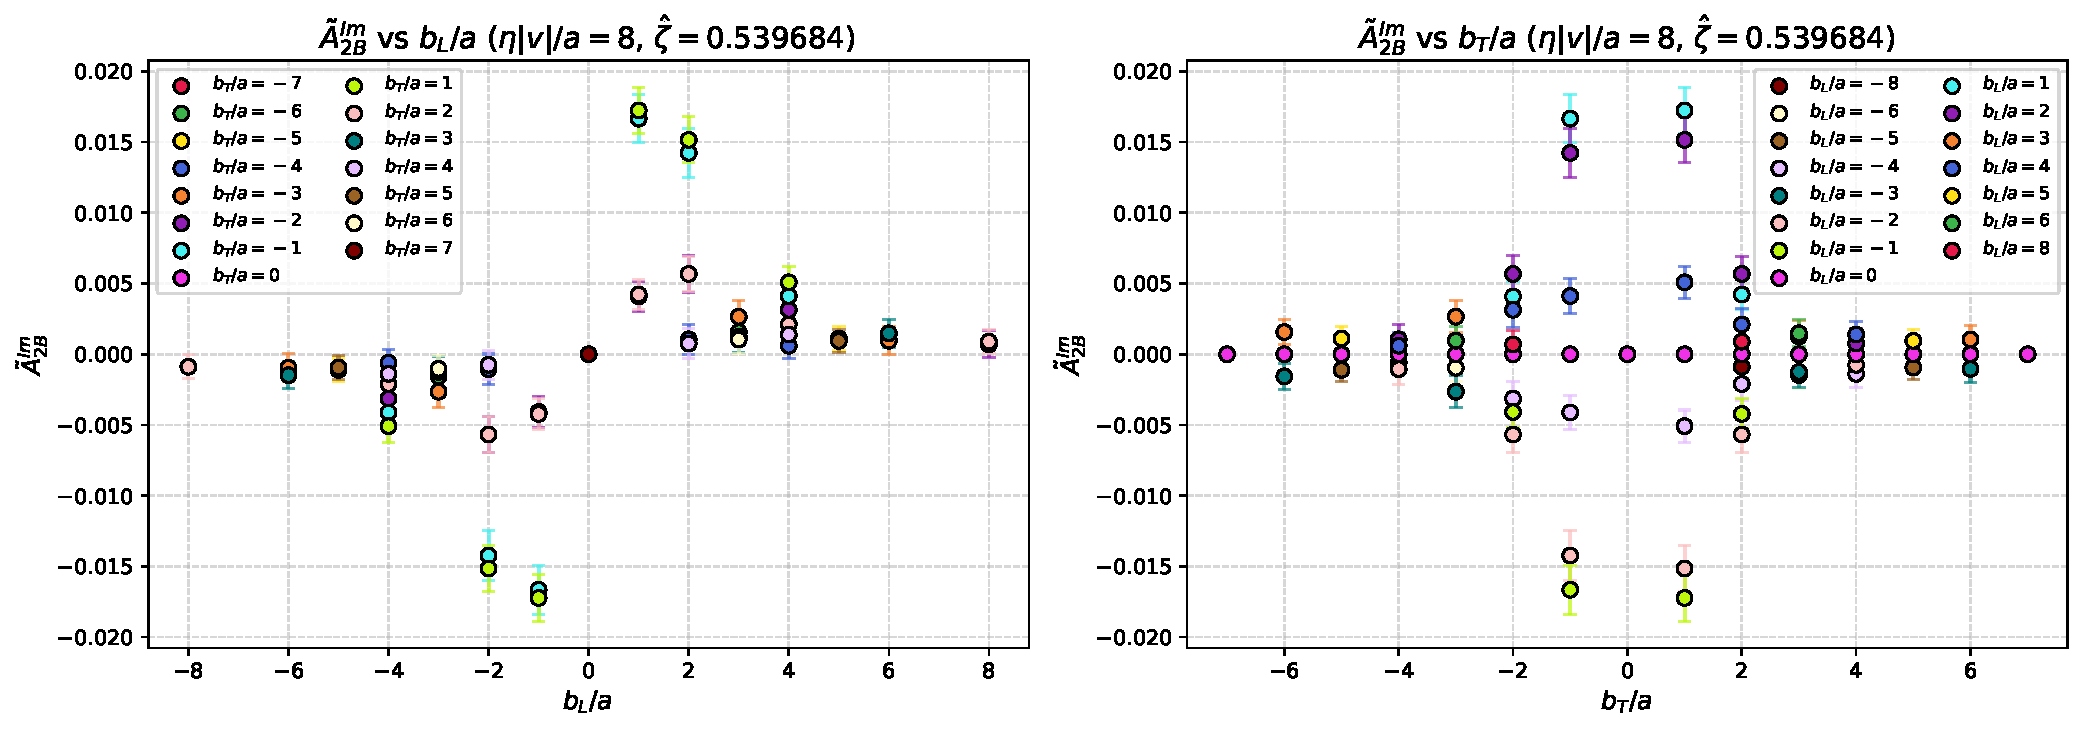
\includegraphics[width=0.98\linewidth,height=0.73\textheight,keepaspectratio]{ImA2B_eta8_PL-3_2D.pdf}\\[1mm]
{\small $\zetahat=0.539684$; $(b_L,b_T)$; $\eta|v|/a=8$ slices}
\figsrc{Thesis, Ch. 5: raw amplitude profiles; complete original panels.}
\end{frame}

\begin{frame}{$\tAmp_{2B}^{\mathrm{Im}}$ at $P_L=-3$: invariant coordinates}
\centering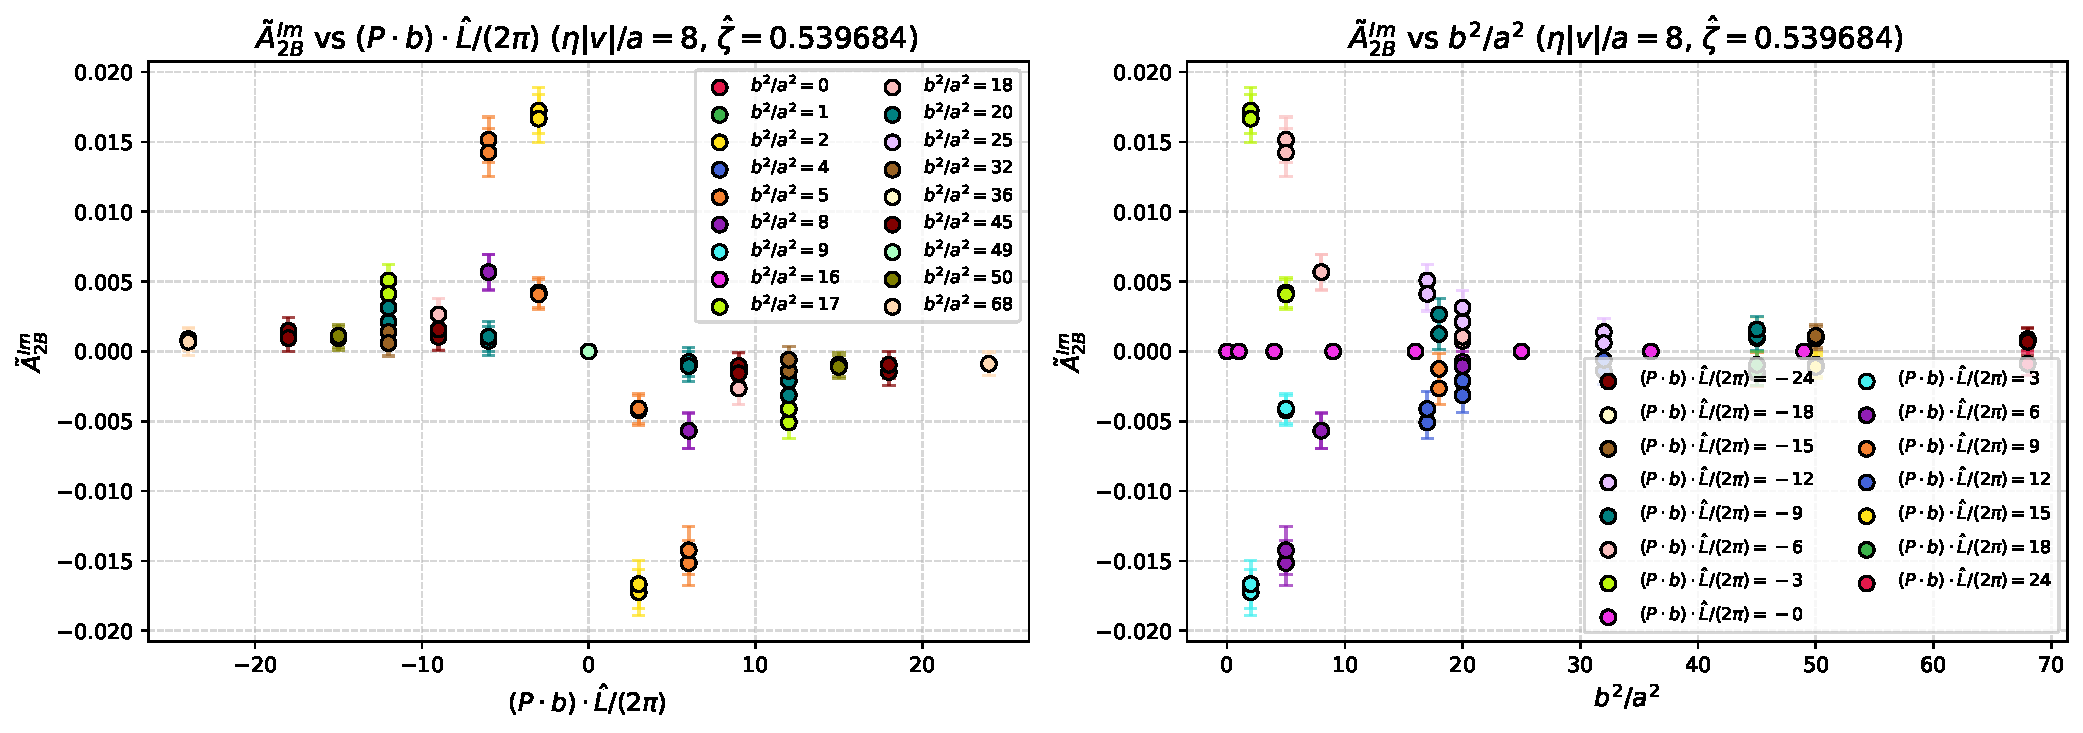
\includegraphics[width=0.98\linewidth,height=0.73\textheight,keepaspectratio]{ImA2B_Pb_bsq_eta8_PL-3_2D.pdf}\\[1mm]
{\small $\zetahat=0.539684$; $(\nu,s)$; $\eta|v|/a=8$ slices}
\figsrc{Thesis, Ch. 5: raw amplitude profiles; complete original panels.}
\end{frame}

\begin{frame}{$\tAmp_{12B}^{\mathrm{Re}}$ at $P_L=-3$: lattice coordinates}
\centering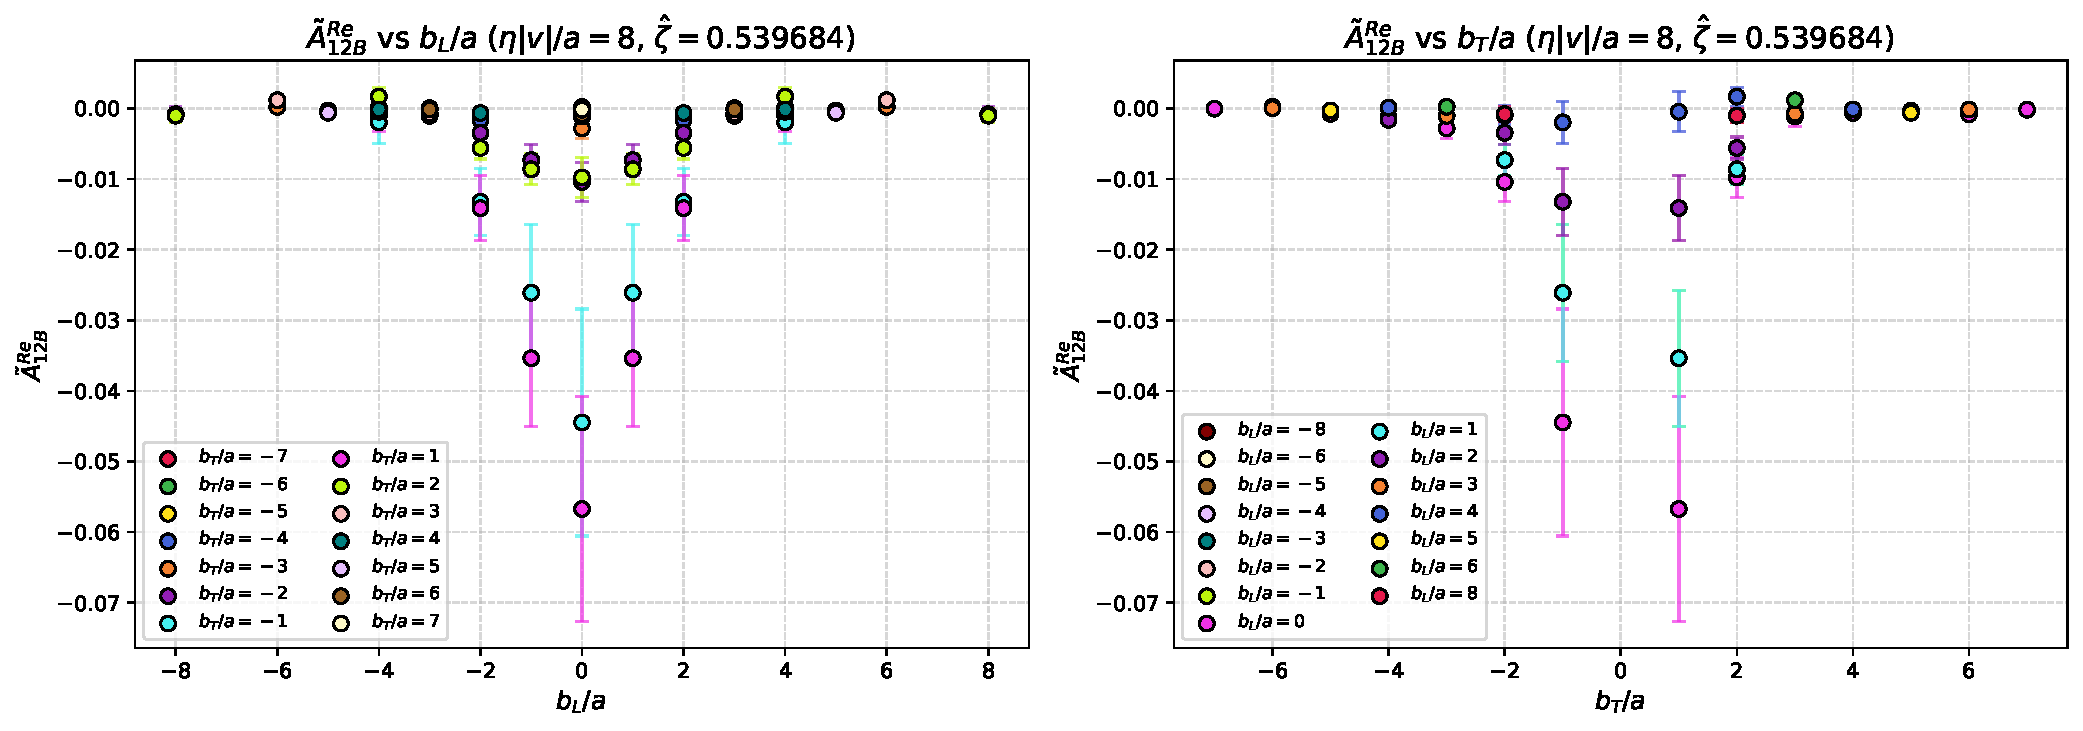
\includegraphics[width=0.98\linewidth,height=0.73\textheight,keepaspectratio]{ReA12B_eta8_PL-3_2D.pdf}\\[1mm]
{\small $\zetahat=0.539684$; $(b_L,b_T)$; $\eta|v|/a=8$ slices}
\figsrc{Thesis, Ch. 5: raw amplitude profiles; complete original panels.}
\end{frame}

\begin{frame}{$\tAmp_{12B}^{\mathrm{Re}}$ at $P_L=-3$: invariant coordinates}
\centering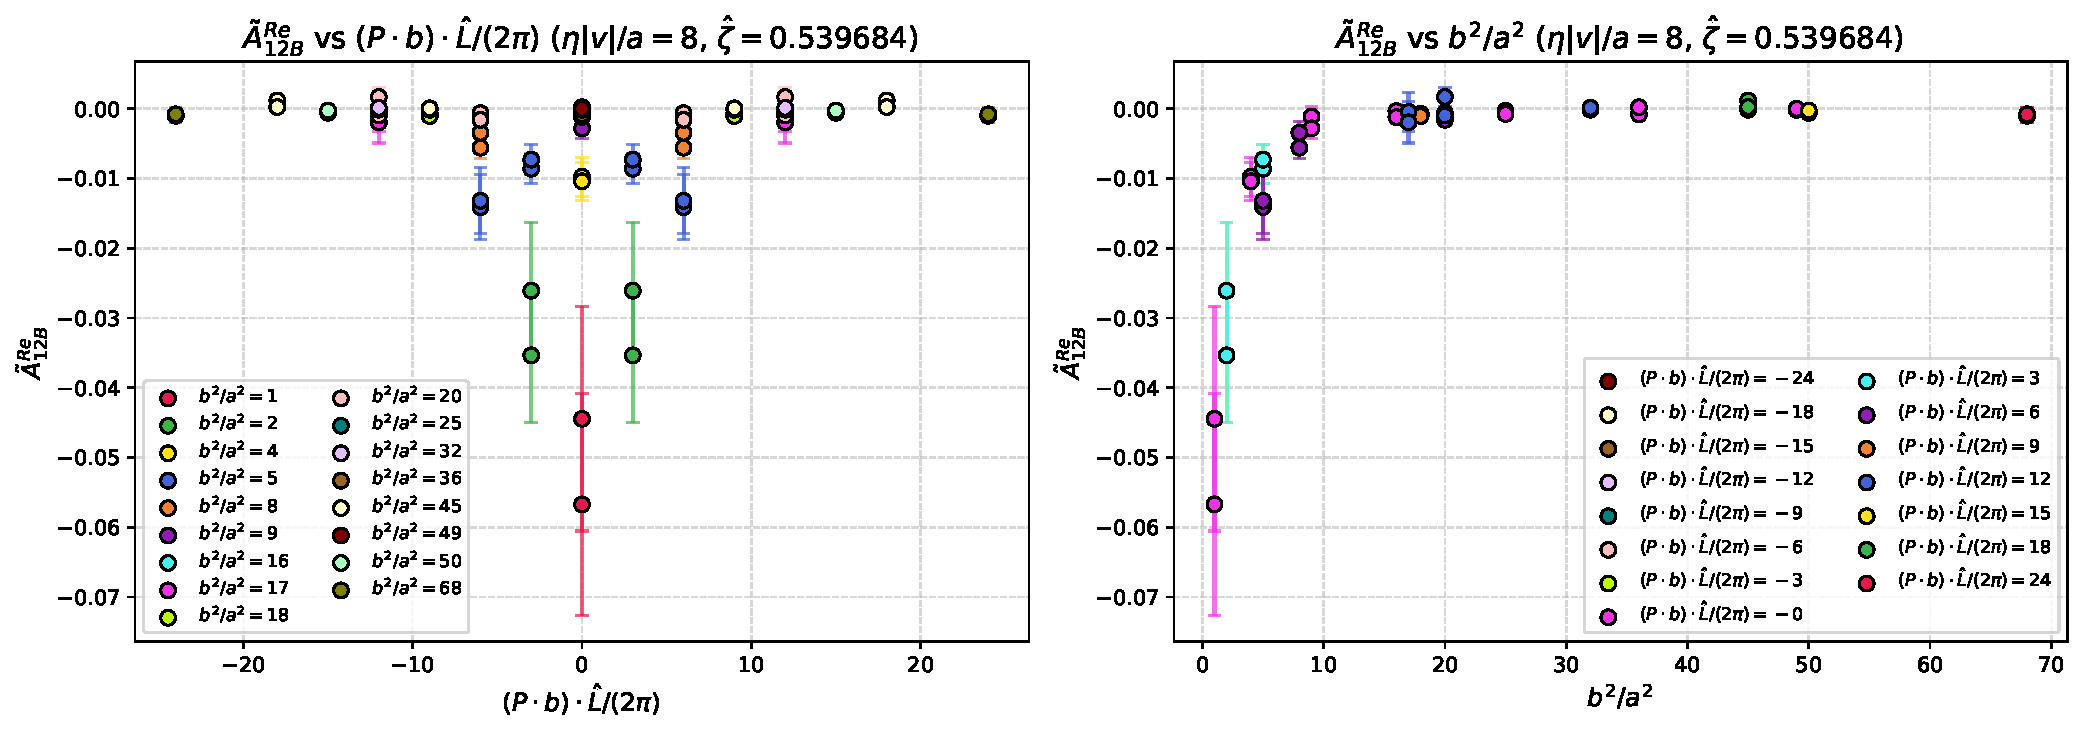
\includegraphics[width=0.98\linewidth,height=0.73\textheight,keepaspectratio]{ReA12B_Pb_bsq_eta8_PL-3_2D.pdf}\\[1mm]
{\small $\zetahat=0.539684$; $(\nu,s)$; $\eta|v|/a=8$ slices}
\figsrc{Thesis, Ch. 5: raw amplitude profiles; complete original panels.}
\end{frame}

\begin{frame}{$\tAmp_{12B}^{\mathrm{Im}}$ at $P_L=-3$: lattice coordinates}
\centering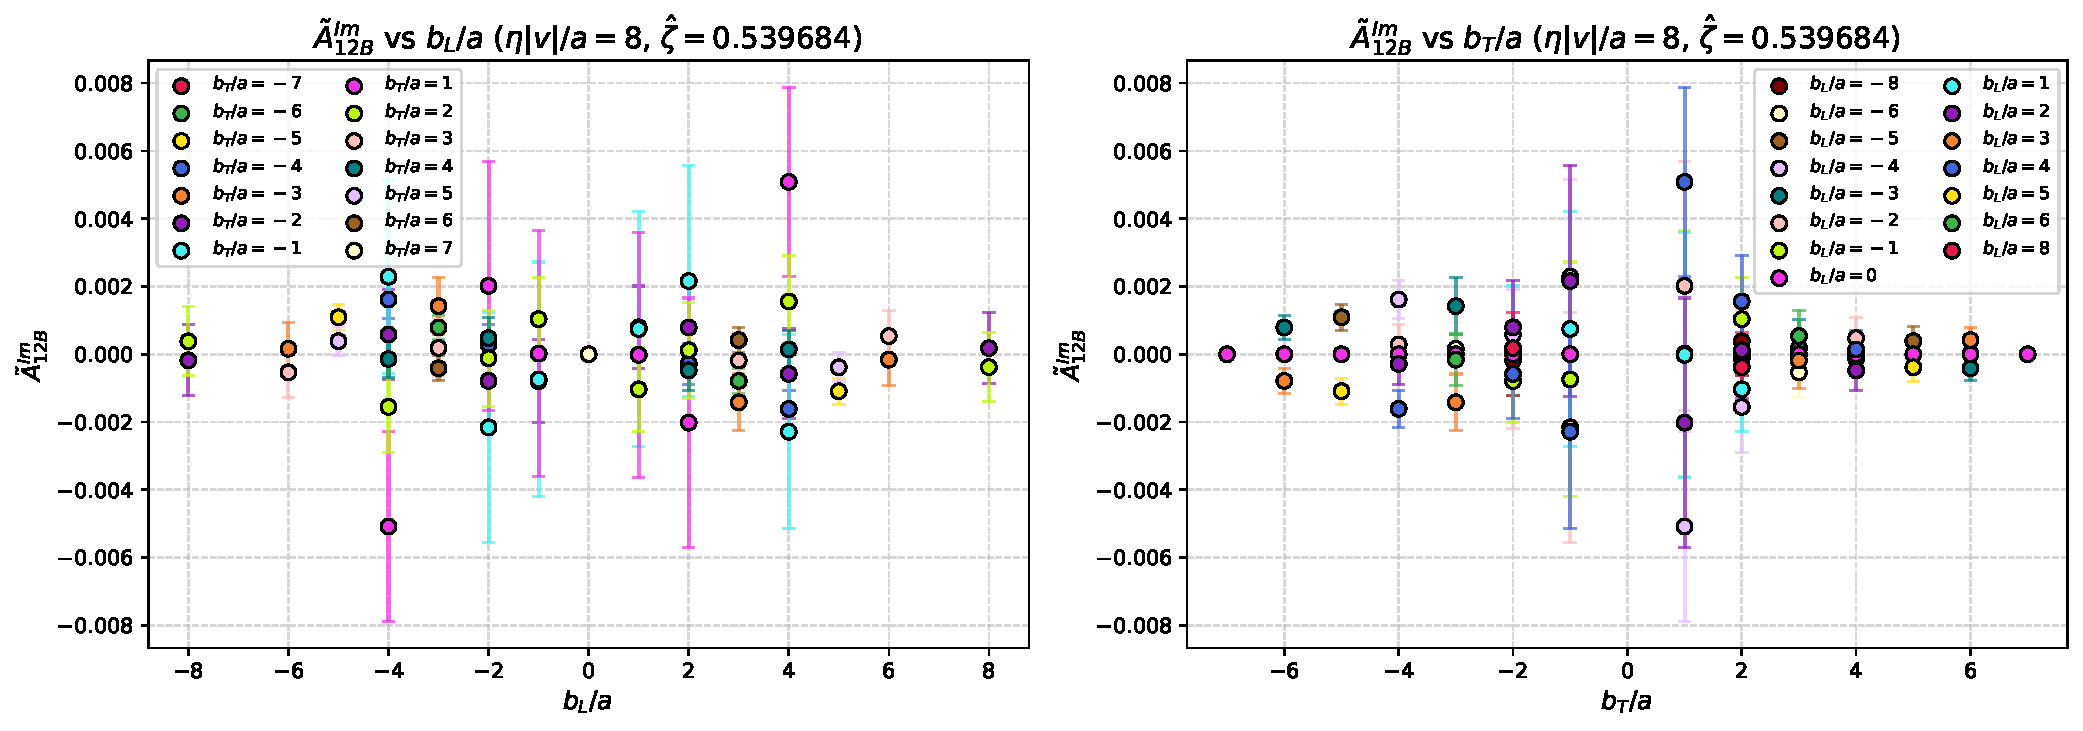
\includegraphics[width=0.98\linewidth,height=0.73\textheight,keepaspectratio]{ImA12B_eta8_PL-3_2D.pdf}\\[1mm]
{\small $\zetahat=0.539684$; $(b_L,b_T)$; $\eta|v|/a=8$ slices}
\figsrc{Thesis, Ch. 5: raw amplitude profiles; complete original panels.}
\end{frame}

\begin{frame}{$\tAmp_{12B}^{\mathrm{Im}}$ at $P_L=-3$: invariant coordinates}
\centering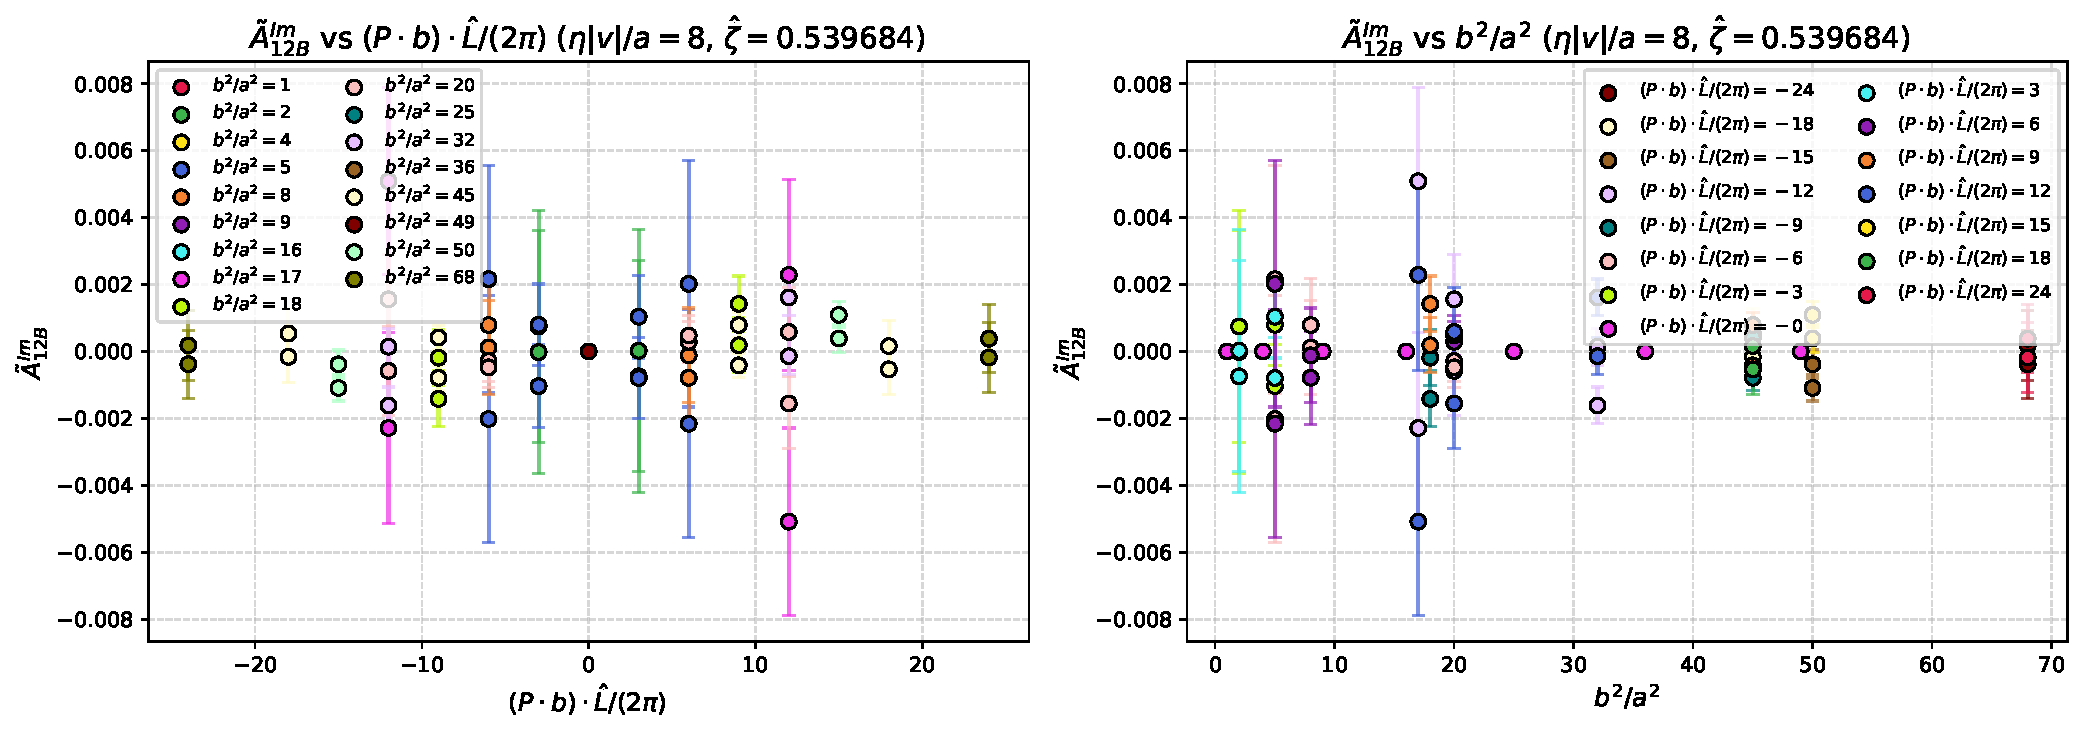
\includegraphics[width=0.98\linewidth,height=0.73\textheight,keepaspectratio]{ImA12B_Pb_bsq_eta8_PL-3_2D.pdf}\\[1mm]
{\small $\zetahat=0.539684$; $(\nu,s)$; $\eta|v|/a=8$ slices}
\figsrc{Thesis, Ch. 5: raw amplitude profiles; complete original panels.}
\end{frame}

\begin{frame}{$\tAmp_{2B}^{\mathrm{Re}}$ at $P_L=-4$: lattice coordinates}
\centering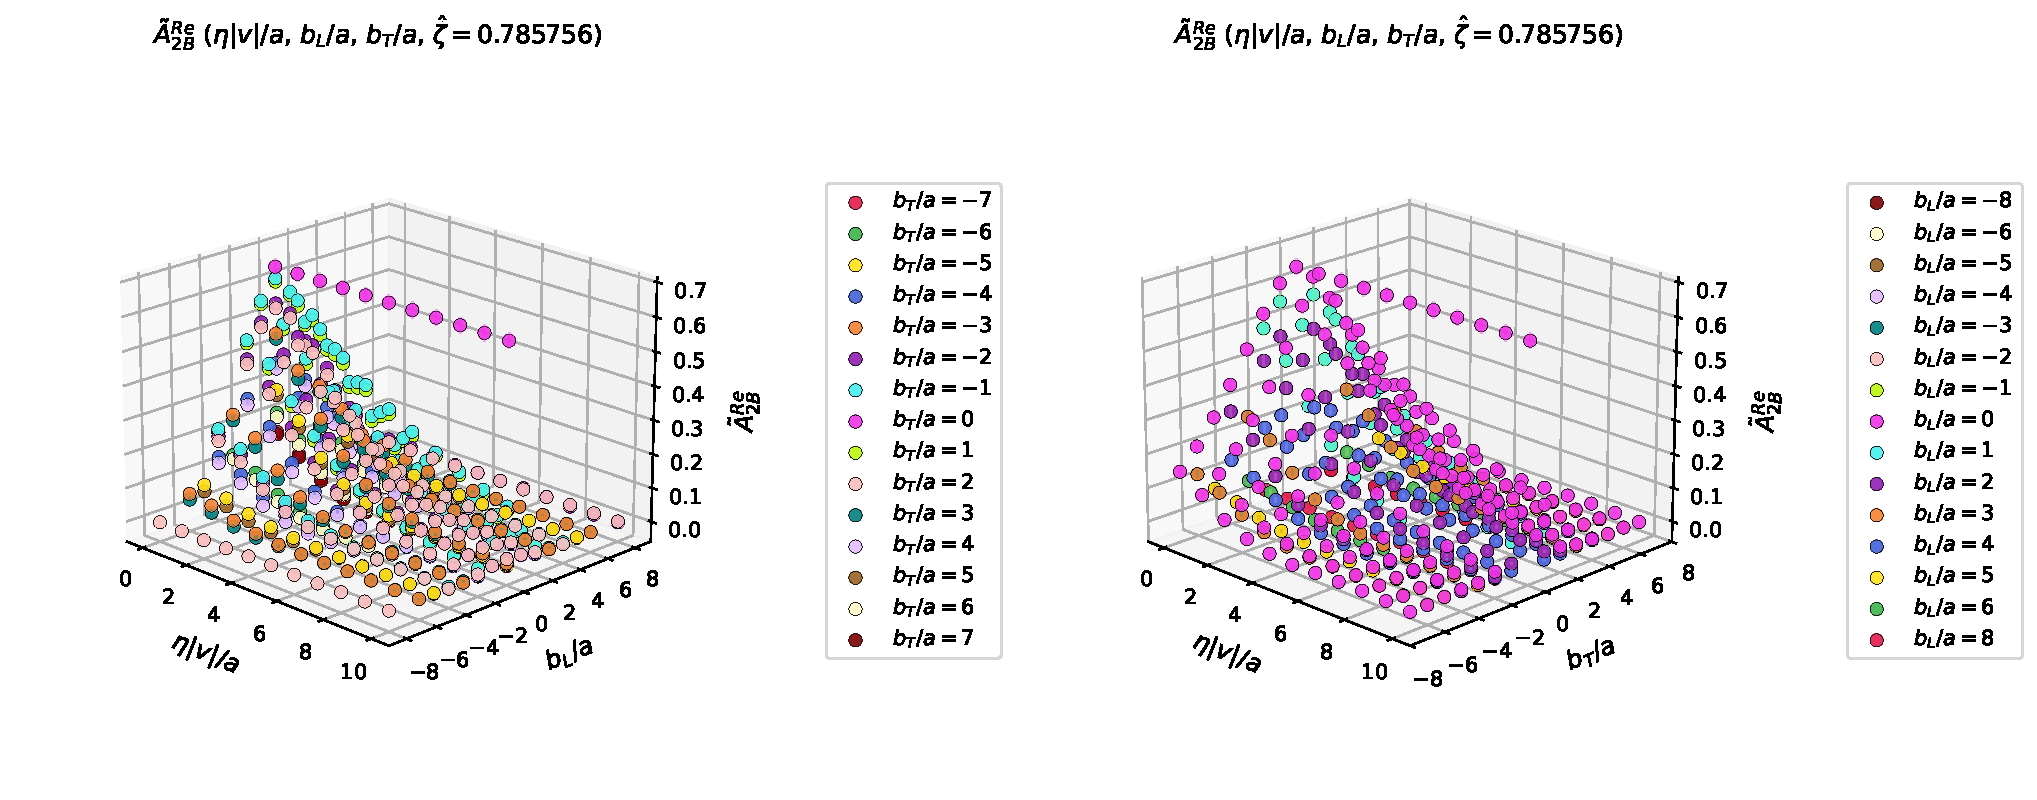
\includegraphics[width=0.98\linewidth,height=0.73\textheight,keepaspectratio]{ReA2B_PL-4_3D.pdf}\\[1mm]
{\small $\zetahat=0.785756$; $(b_L,b_T)$; staple-length dependence}
\figsrc{Thesis, Ch. 5: raw amplitude profiles; complete original panels.}
\end{frame}

\begin{frame}{$\tAmp_{2B}^{\mathrm{Re}}$ at $P_L=-4$: invariant coordinates}
\centering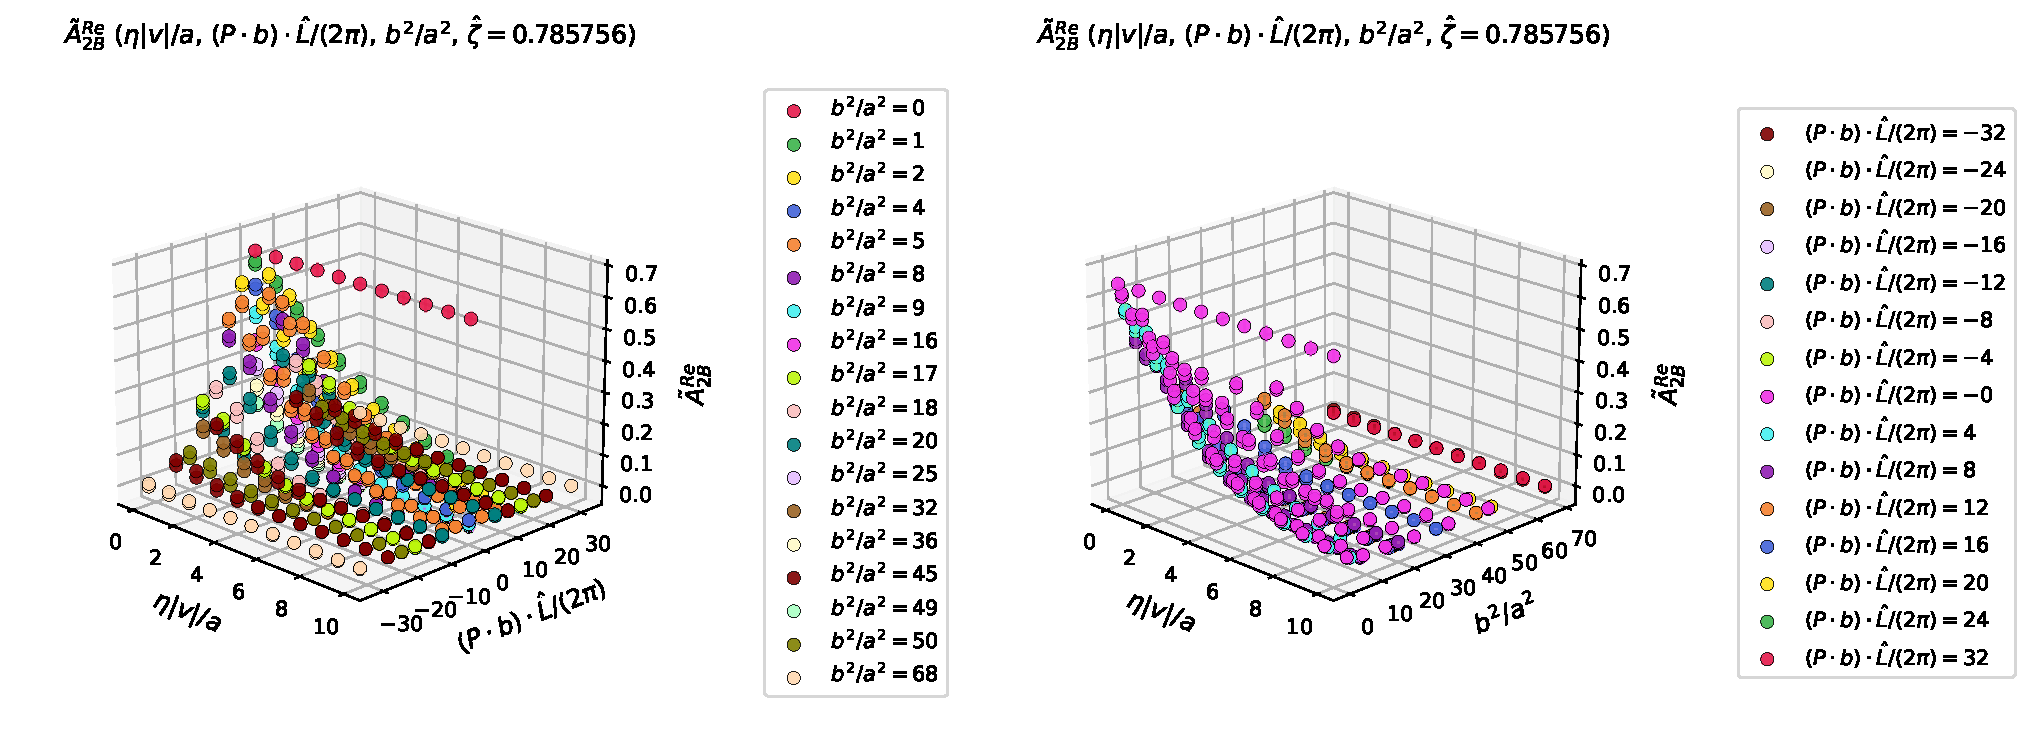
\includegraphics[width=0.98\linewidth,height=0.73\textheight,keepaspectratio]{ReA2B_Pb_bsq_PL-4_3D.pdf}\\[1mm]
{\small $\zetahat=0.785756$; $(\nu,s)$; staple-length dependence}
\figsrc{Thesis, Ch. 5: raw amplitude profiles; complete original panels.}
\end{frame}

\begin{frame}{$\tAmp_{2B}^{\mathrm{Im}}$ at $P_L=-4$: lattice coordinates}
\centering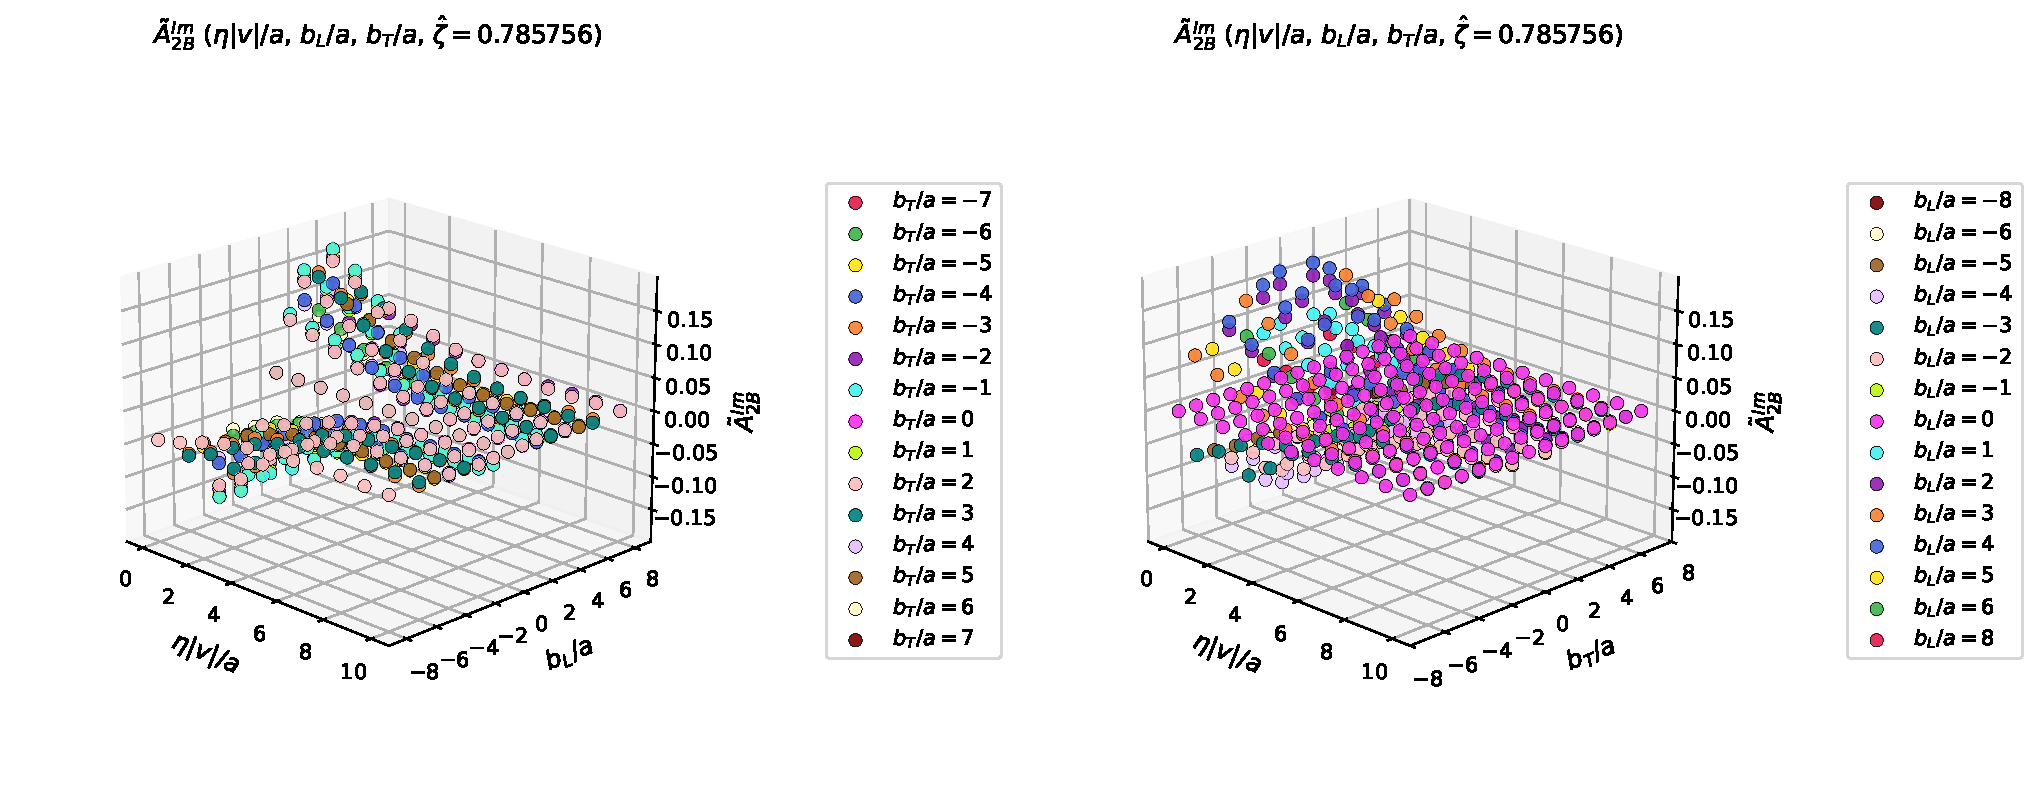
\includegraphics[width=0.98\linewidth,height=0.73\textheight,keepaspectratio]{ImA2B_PL-4_3D.pdf}\\[1mm]
{\small $\zetahat=0.785756$; $(b_L,b_T)$; staple-length dependence}
\figsrc{Thesis, Ch. 5: raw amplitude profiles; complete original panels.}
\end{frame}

\begin{frame}{$\tAmp_{2B}^{\mathrm{Im}}$ at $P_L=-4$: invariant coordinates}
\centering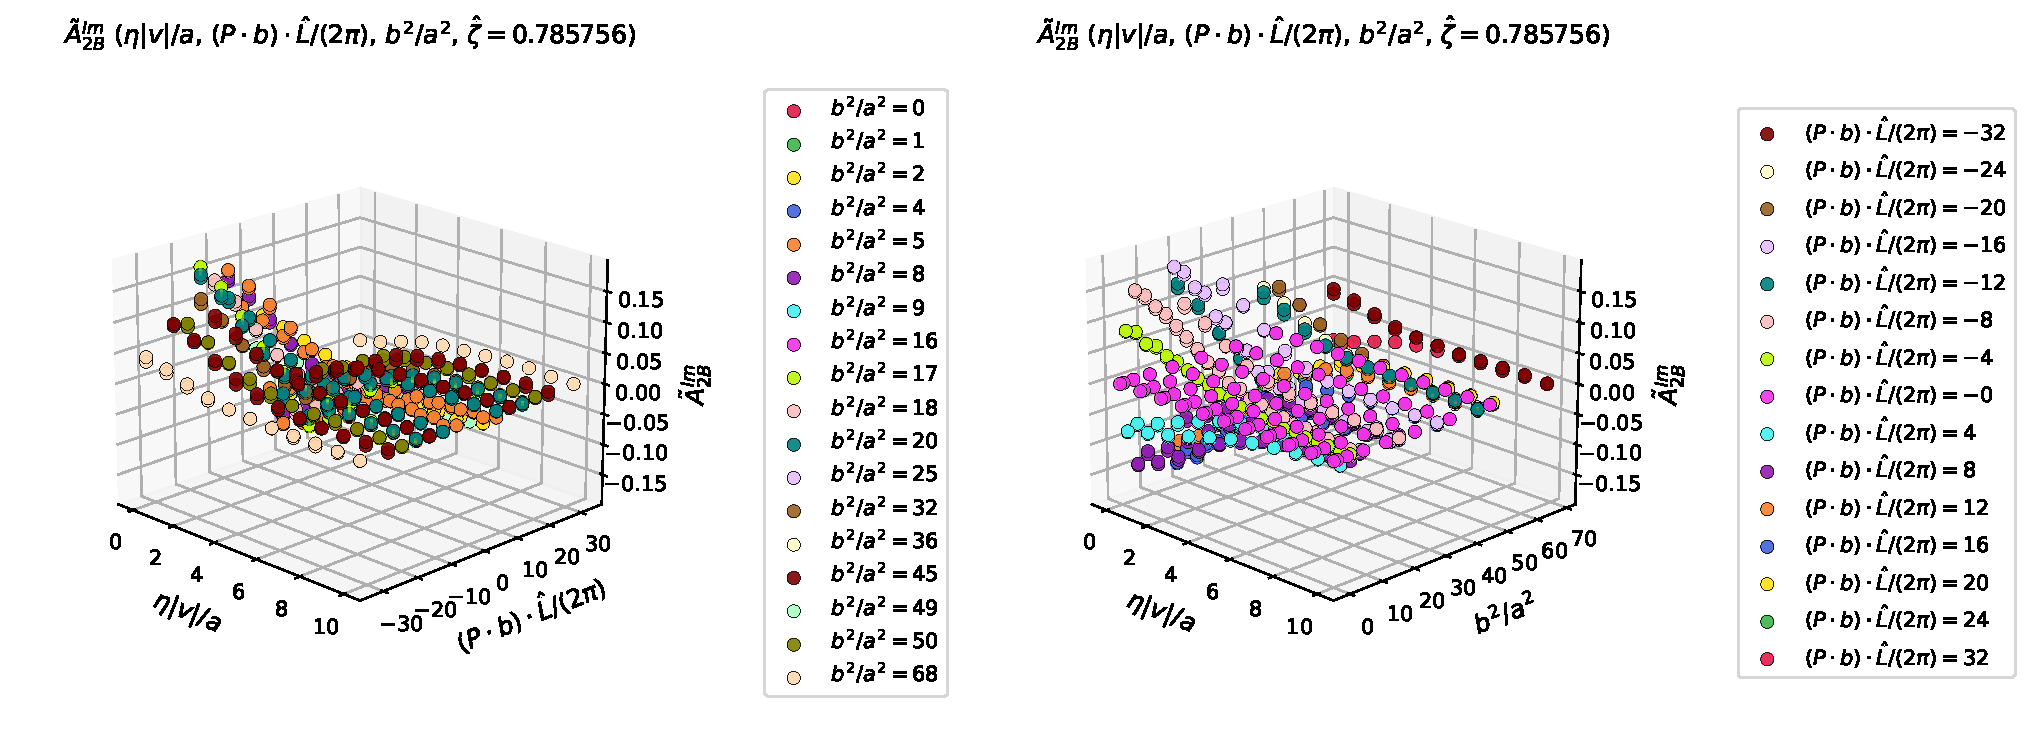
\includegraphics[width=0.98\linewidth,height=0.73\textheight,keepaspectratio]{ImA2B_Pb_bsq_PL-4_3D.pdf}\\[1mm]
{\small $\zetahat=0.785756$; $(\nu,s)$; staple-length dependence}
\figsrc{Thesis, Ch. 5: raw amplitude profiles; complete original panels.}
\end{frame}

\begin{frame}{$\tAmp_{12B}^{\mathrm{Re}}$ at $P_L=-4$: lattice coordinates}
\centering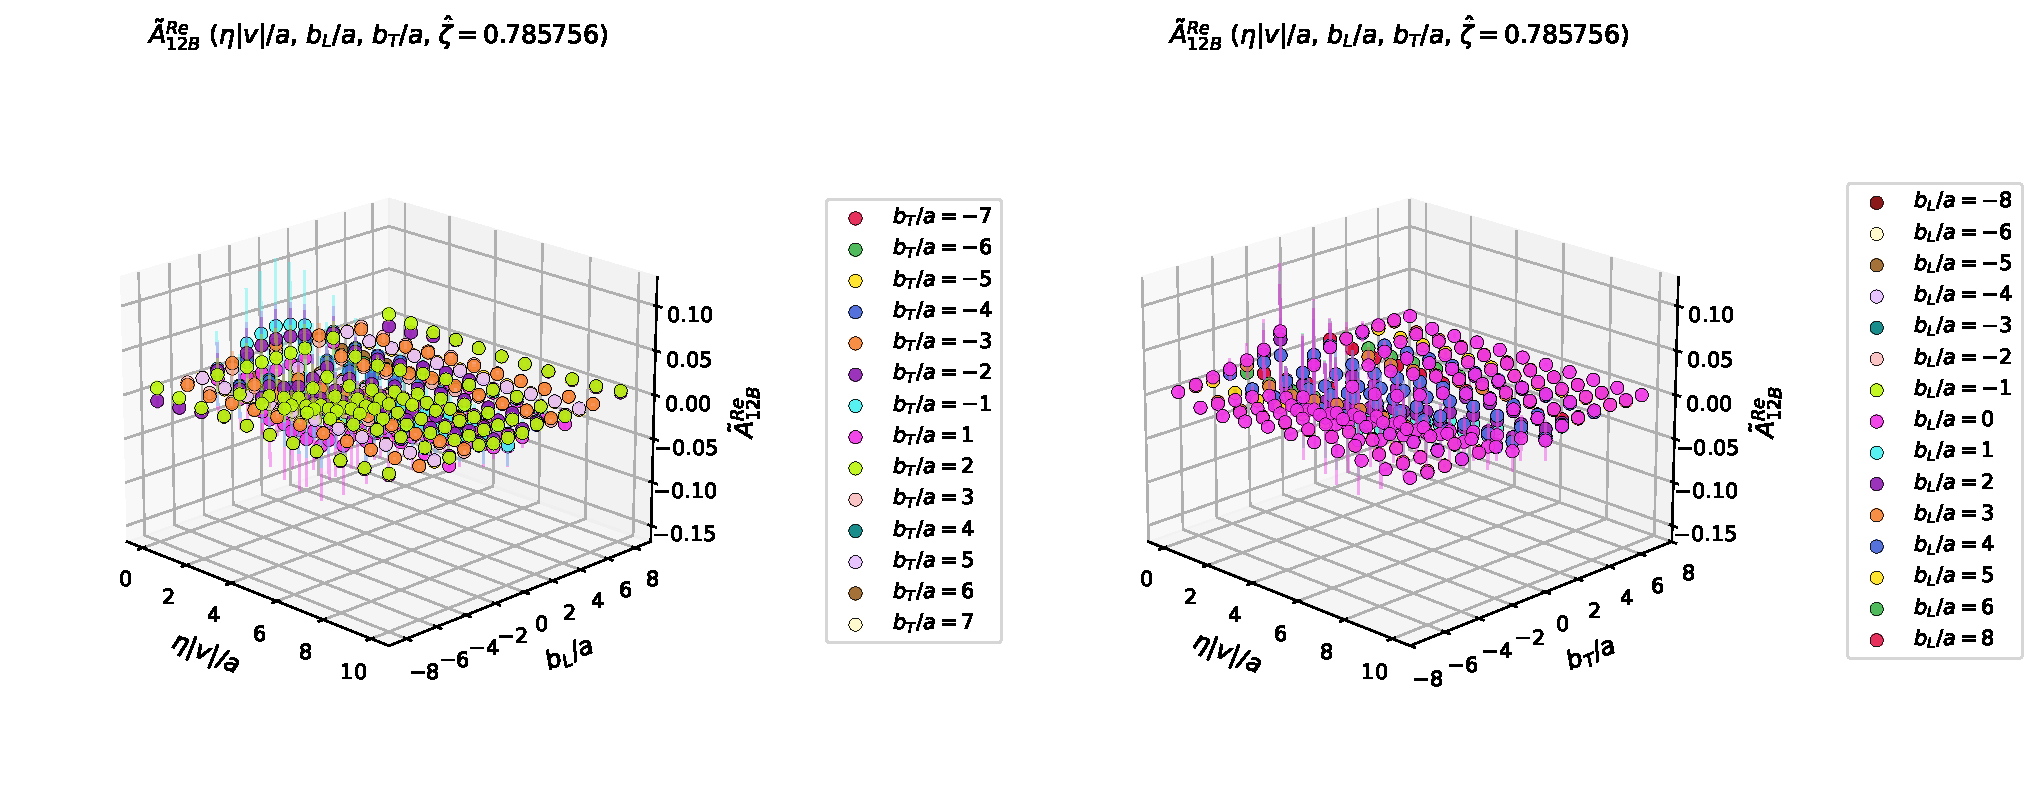
\includegraphics[width=0.98\linewidth,height=0.73\textheight,keepaspectratio]{ReA12B_PL-4_3D.pdf}\\[1mm]
{\small $\zetahat=0.785756$; $(b_L,b_T)$; staple-length dependence}
\figsrc{Thesis, Ch. 5: raw amplitude profiles; complete original panels.}
\end{frame}

\begin{frame}{$\tAmp_{12B}^{\mathrm{Re}}$ at $P_L=-4$: invariant coordinates}
\centering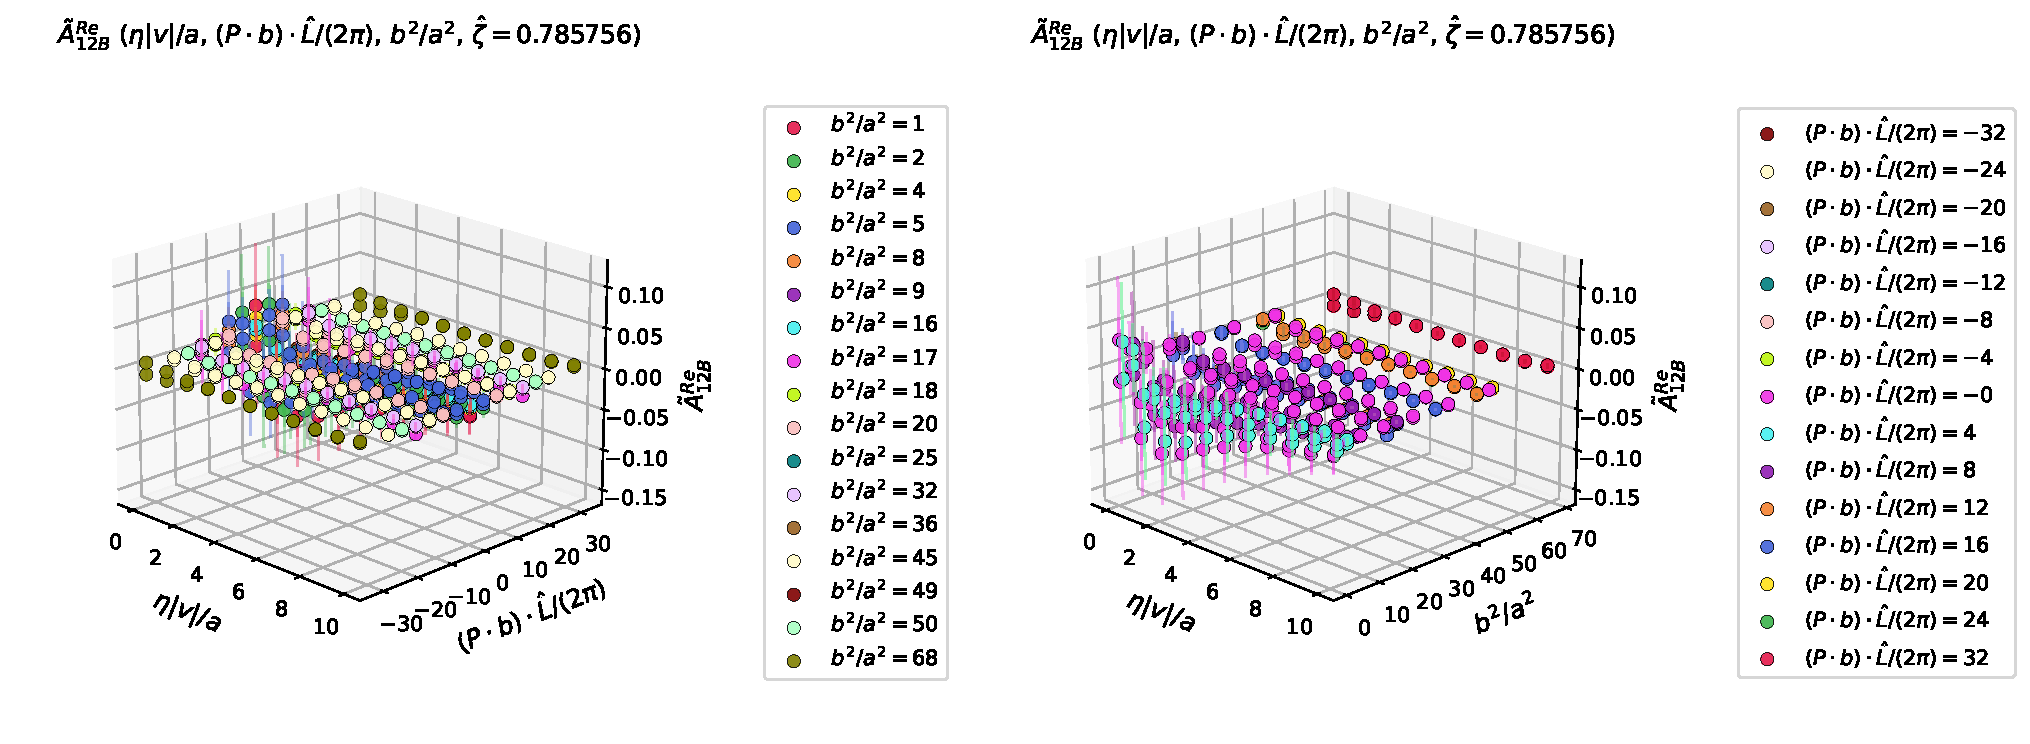
\includegraphics[width=0.98\linewidth,height=0.73\textheight,keepaspectratio]{ReA12B_Pb_bsq_PL-4_3D.pdf}\\[1mm]
{\small $\zetahat=0.785756$; $(\nu,s)$; staple-length dependence}
\figsrc{Thesis, Ch. 5: raw amplitude profiles; complete original panels.}
\end{frame}

\begin{frame}{$\tAmp_{12B}^{\mathrm{Im}}$ at $P_L=-4$: lattice coordinates}
\centering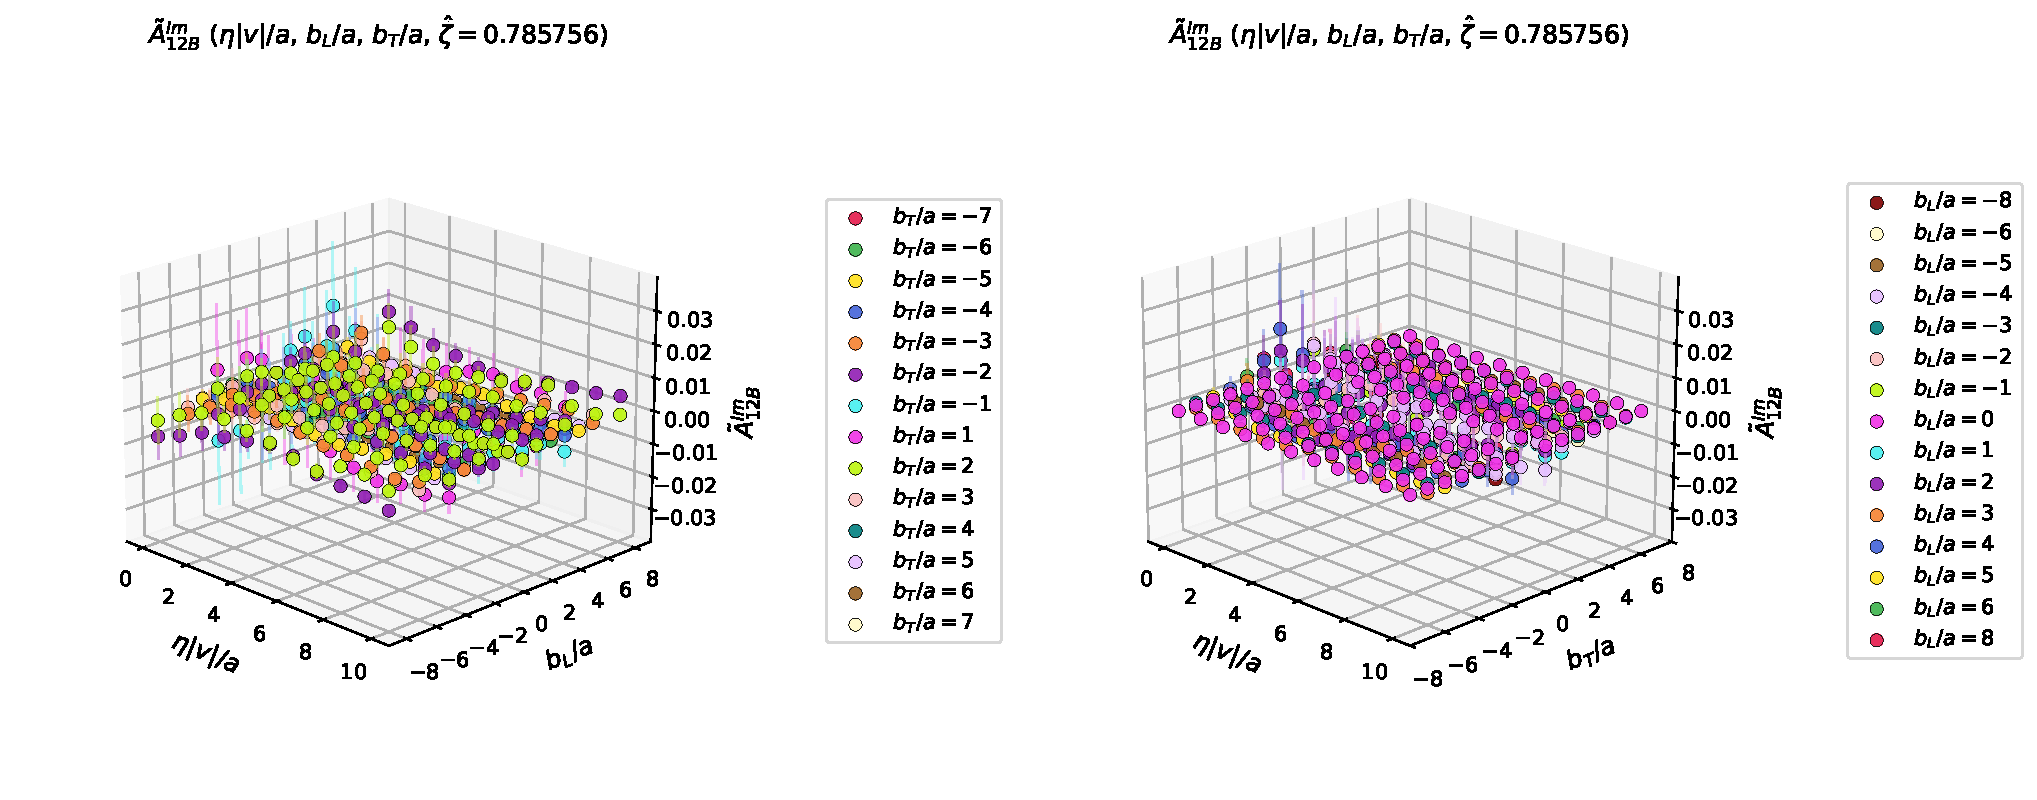
\includegraphics[width=0.98\linewidth,height=0.73\textheight,keepaspectratio]{ImA12B_PL-4_3D.pdf}\\[1mm]
{\small $\zetahat=0.785756$; $(b_L,b_T)$; staple-length dependence}
\figsrc{Thesis, Ch. 5: raw amplitude profiles; complete original panels.}
\end{frame}

\begin{frame}{$\tAmp_{12B}^{\mathrm{Im}}$ at $P_L=-4$: invariant coordinates}
\centering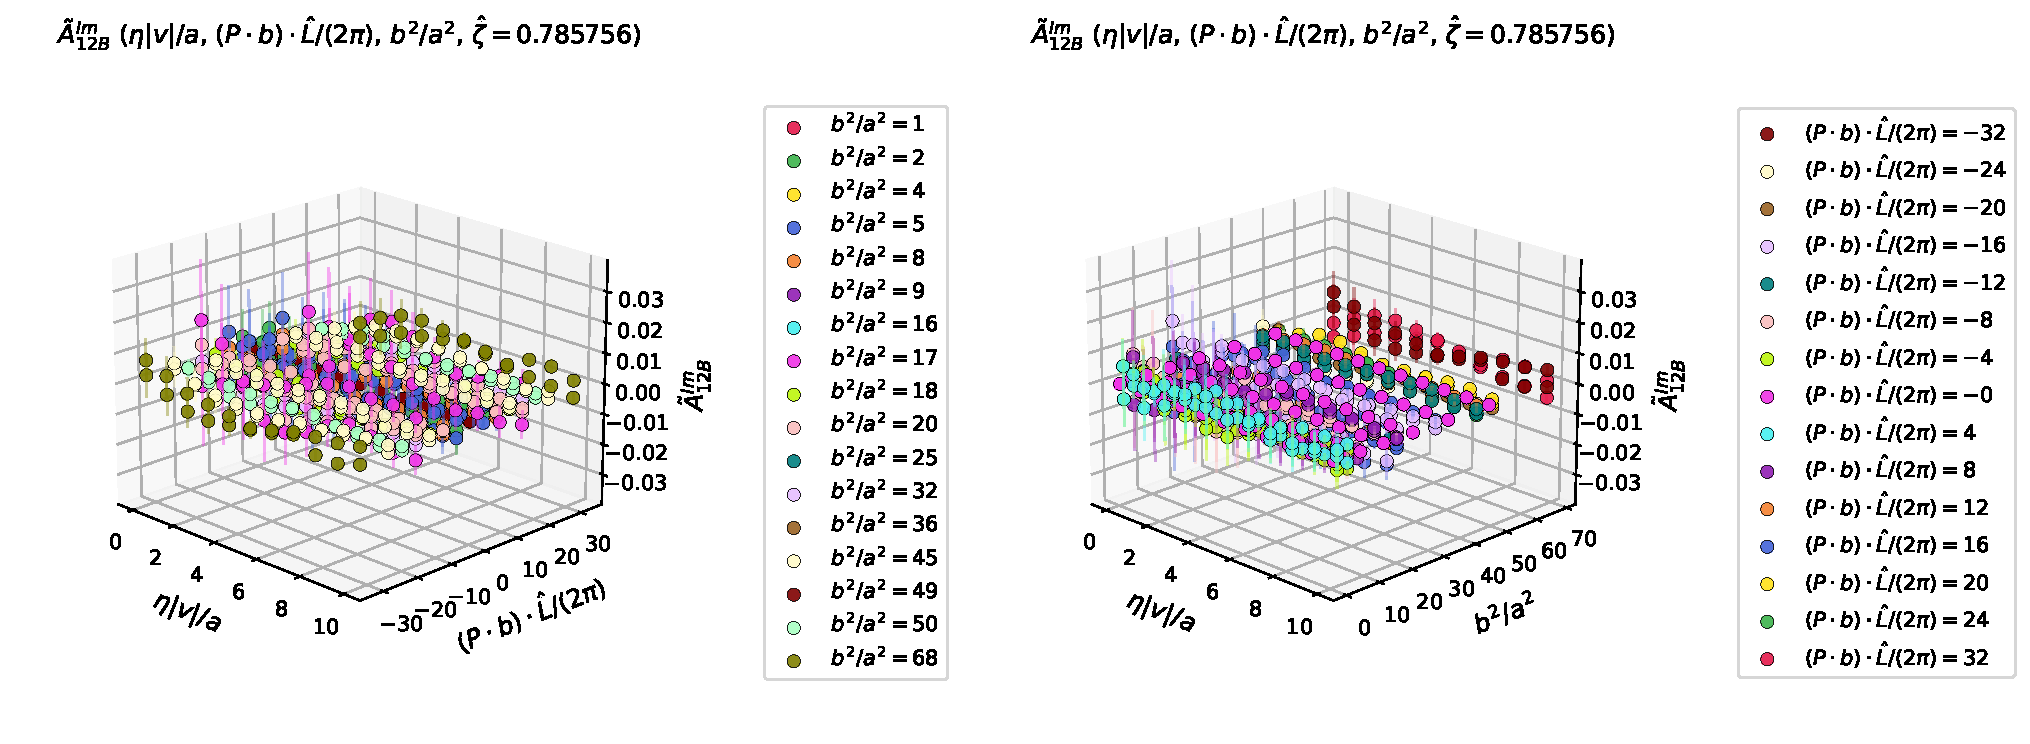
\includegraphics[width=0.98\linewidth,height=0.73\textheight,keepaspectratio]{ImA12B_Pb_bsq_PL-4_3D.pdf}\\[1mm]
{\small $\zetahat=0.785756$; $(\nu,s)$; staple-length dependence}
\figsrc{Thesis, Ch. 5: raw amplitude profiles; complete original panels.}
\end{frame}

\begin{frame}{$\tAmp_{2B}^{\mathrm{Re}}$ at $P_L=-4$: lattice coordinates}
\centering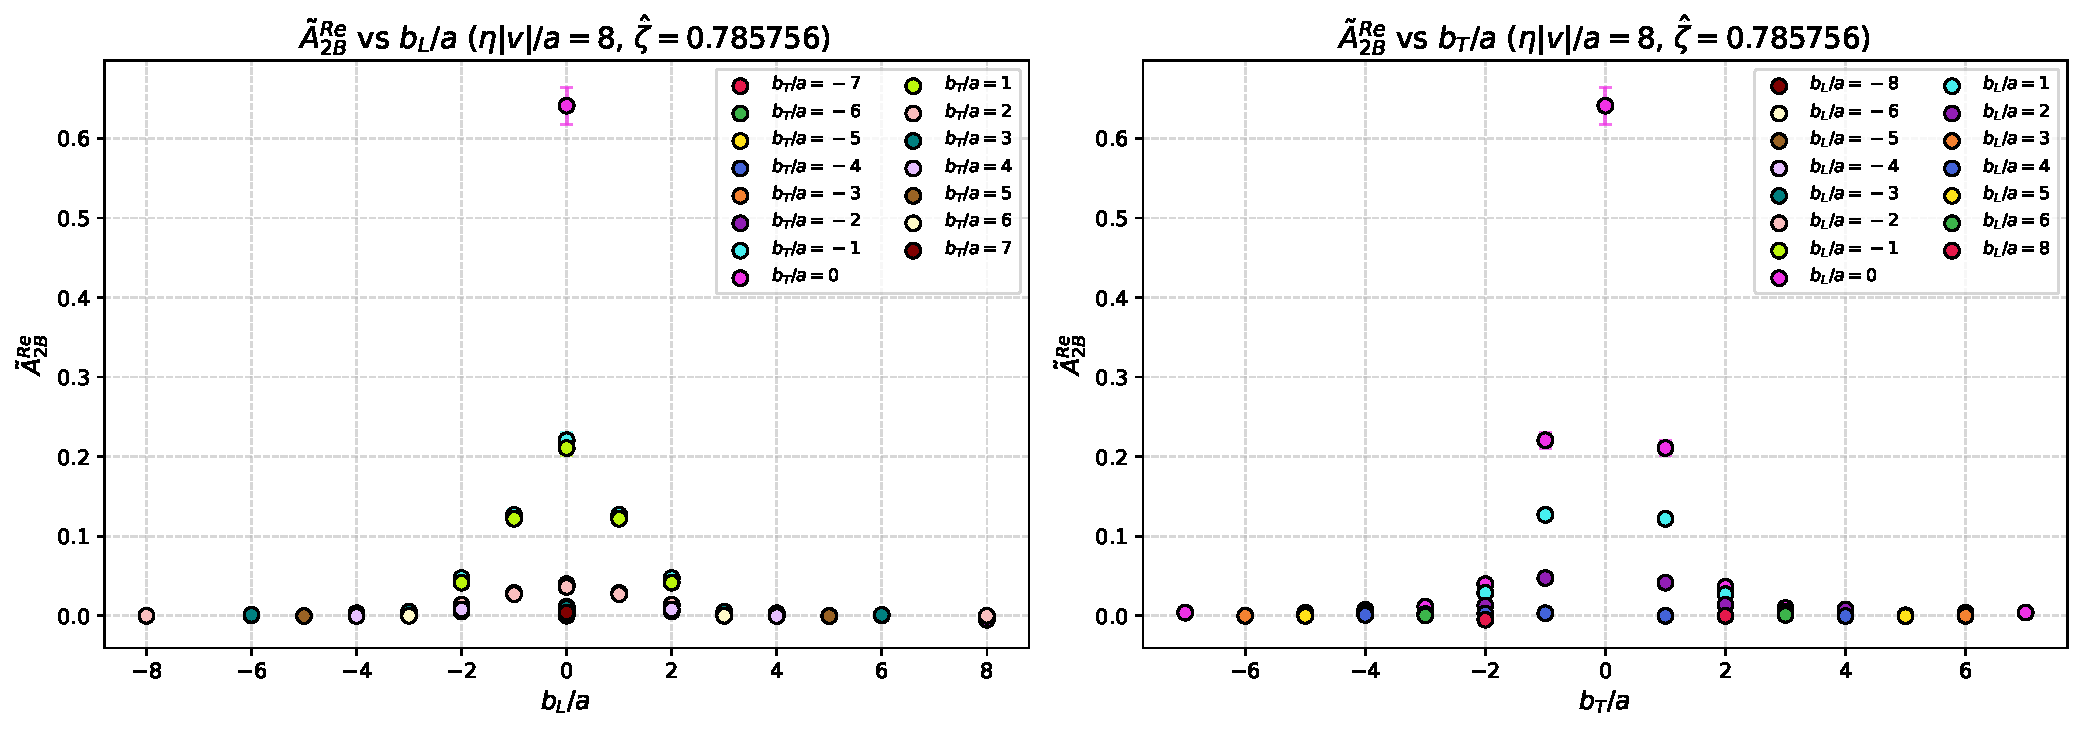
\includegraphics[width=0.98\linewidth,height=0.73\textheight,keepaspectratio]{ReA2B_eta8_PL-4_2D.pdf}\\[1mm]
{\small $\zetahat=0.785756$; $(b_L,b_T)$; $\eta|v|/a=8$ slices}
\figsrc{Thesis, Ch. 5: raw amplitude profiles; complete original panels.}
\end{frame}

\begin{frame}{$\tAmp_{2B}^{\mathrm{Re}}$ at $P_L=-4$: invariant coordinates}
\centering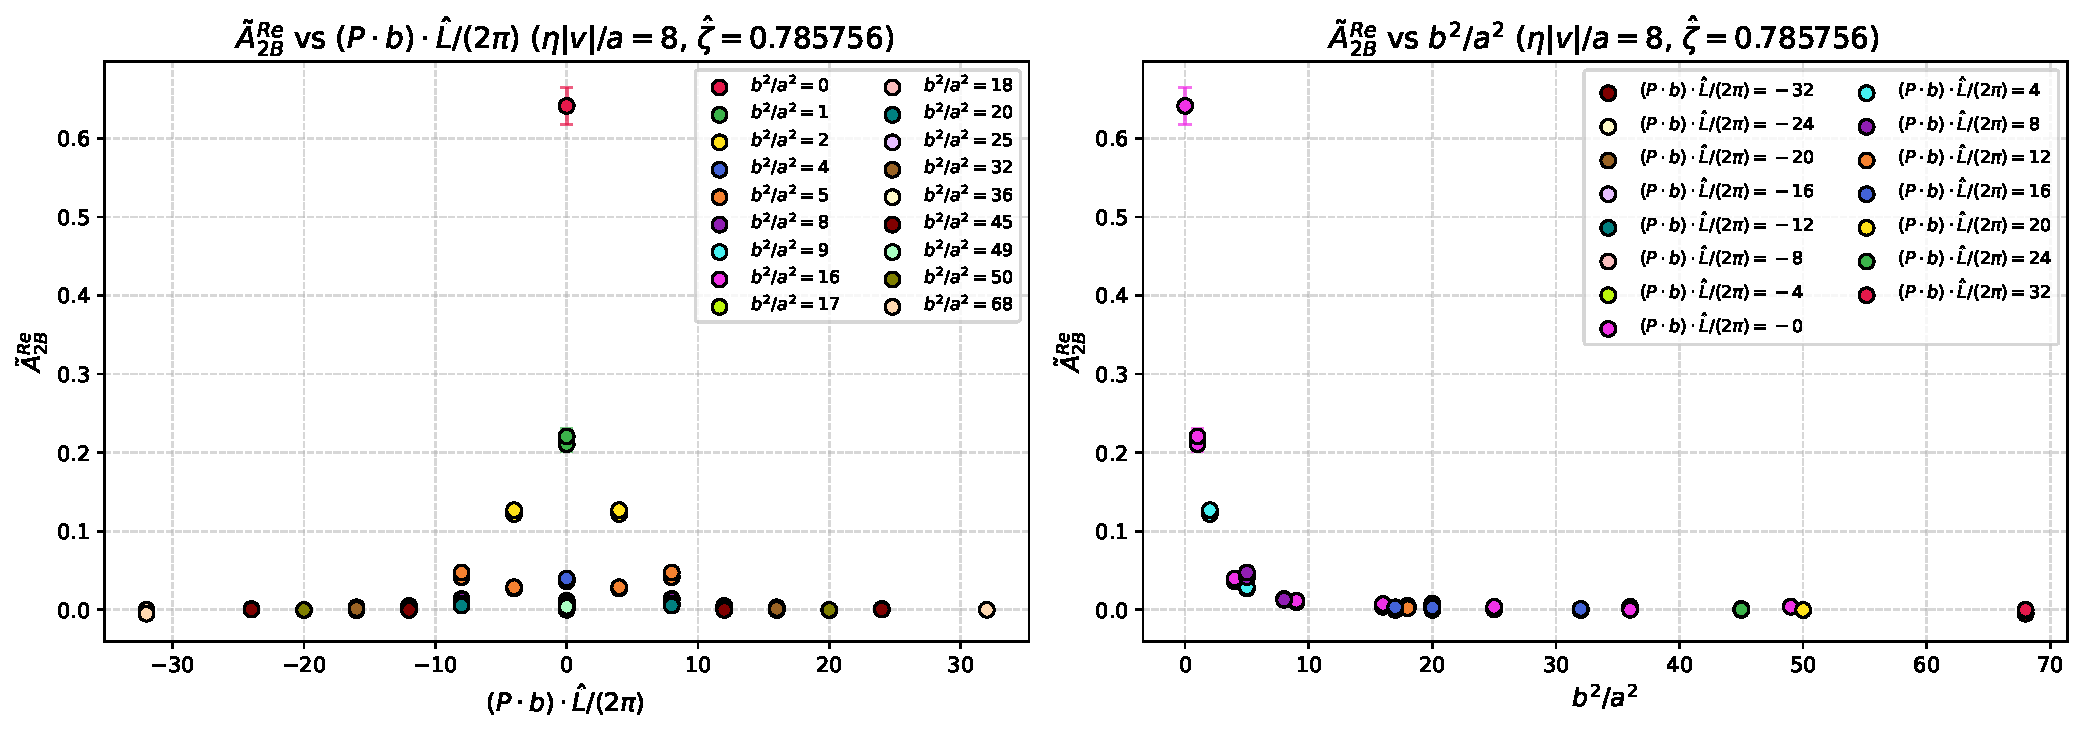
\includegraphics[width=0.98\linewidth,height=0.73\textheight,keepaspectratio]{ReA2B_Pb_bsq_eta8_PL-4_2D.pdf}\\[1mm]
{\small $\zetahat=0.785756$; $(\nu,s)$; $\eta|v|/a=8$ slices}
\figsrc{Thesis, Ch. 5: raw amplitude profiles; complete original panels.}
\end{frame}

\begin{frame}{$\tAmp_{2B}^{\mathrm{Im}}$ at $P_L=-4$: lattice coordinates}
\centering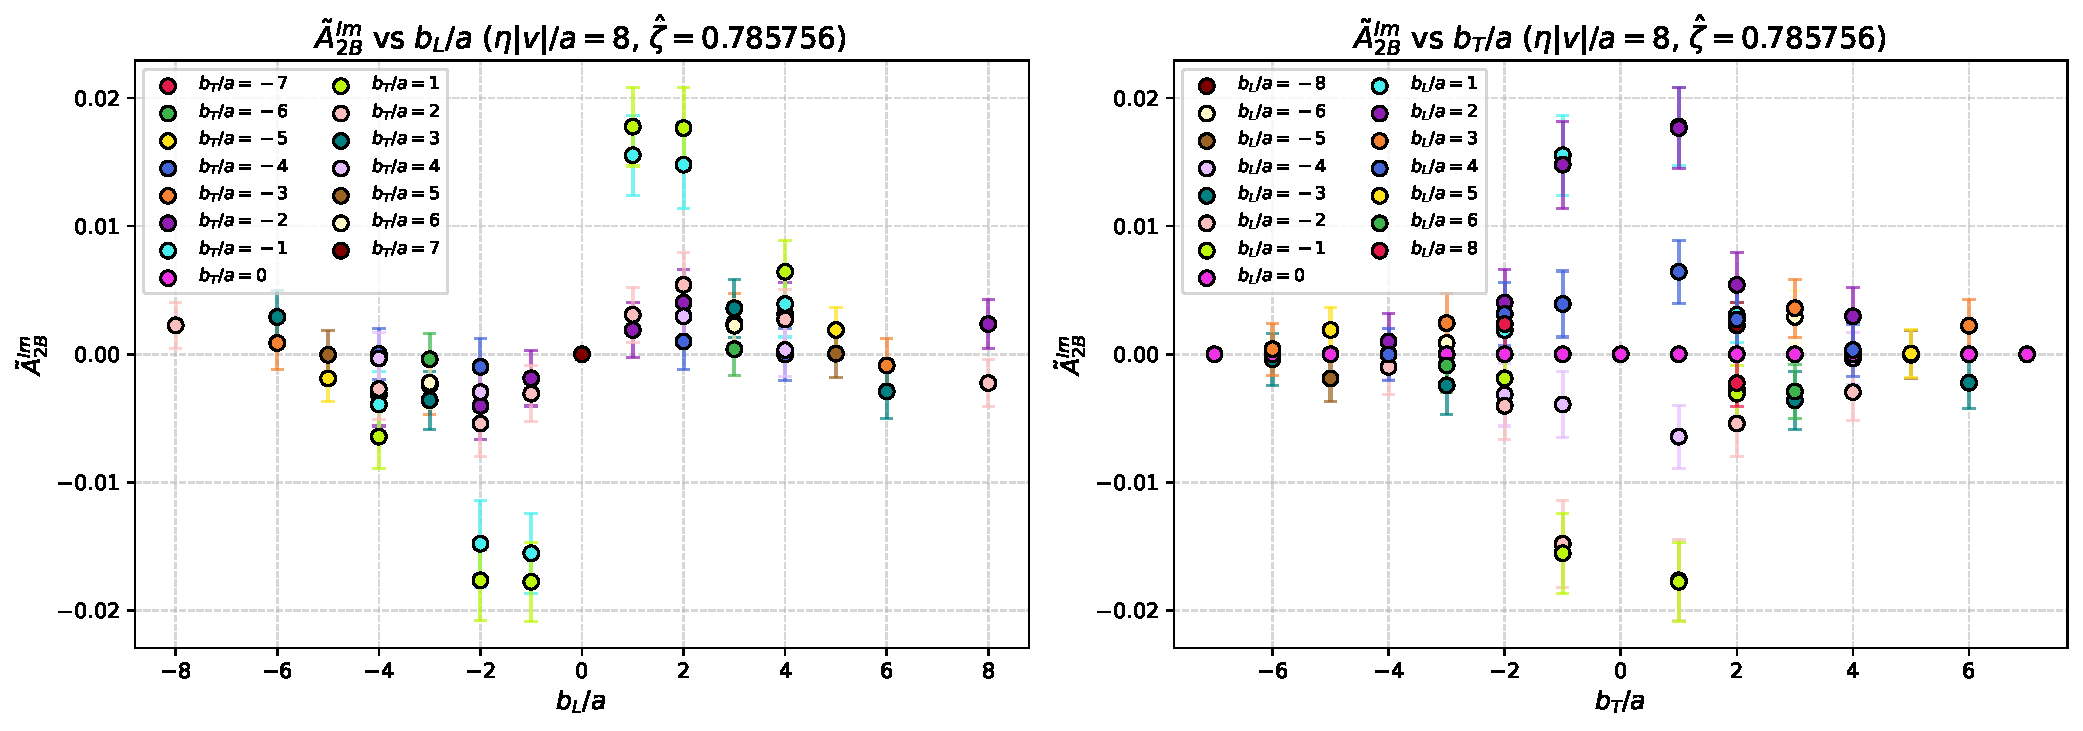
\includegraphics[width=0.98\linewidth,height=0.73\textheight,keepaspectratio]{ImA2B_eta8_PL-4_2D.pdf}\\[1mm]
{\small $\zetahat=0.785756$; $(b_L,b_T)$; $\eta|v|/a=8$ slices}
\figsrc{Thesis, Ch. 5: raw amplitude profiles; complete original panels.}
\end{frame}

\begin{frame}{$\tAmp_{2B}^{\mathrm{Im}}$ at $P_L=-4$: invariant coordinates}
\centering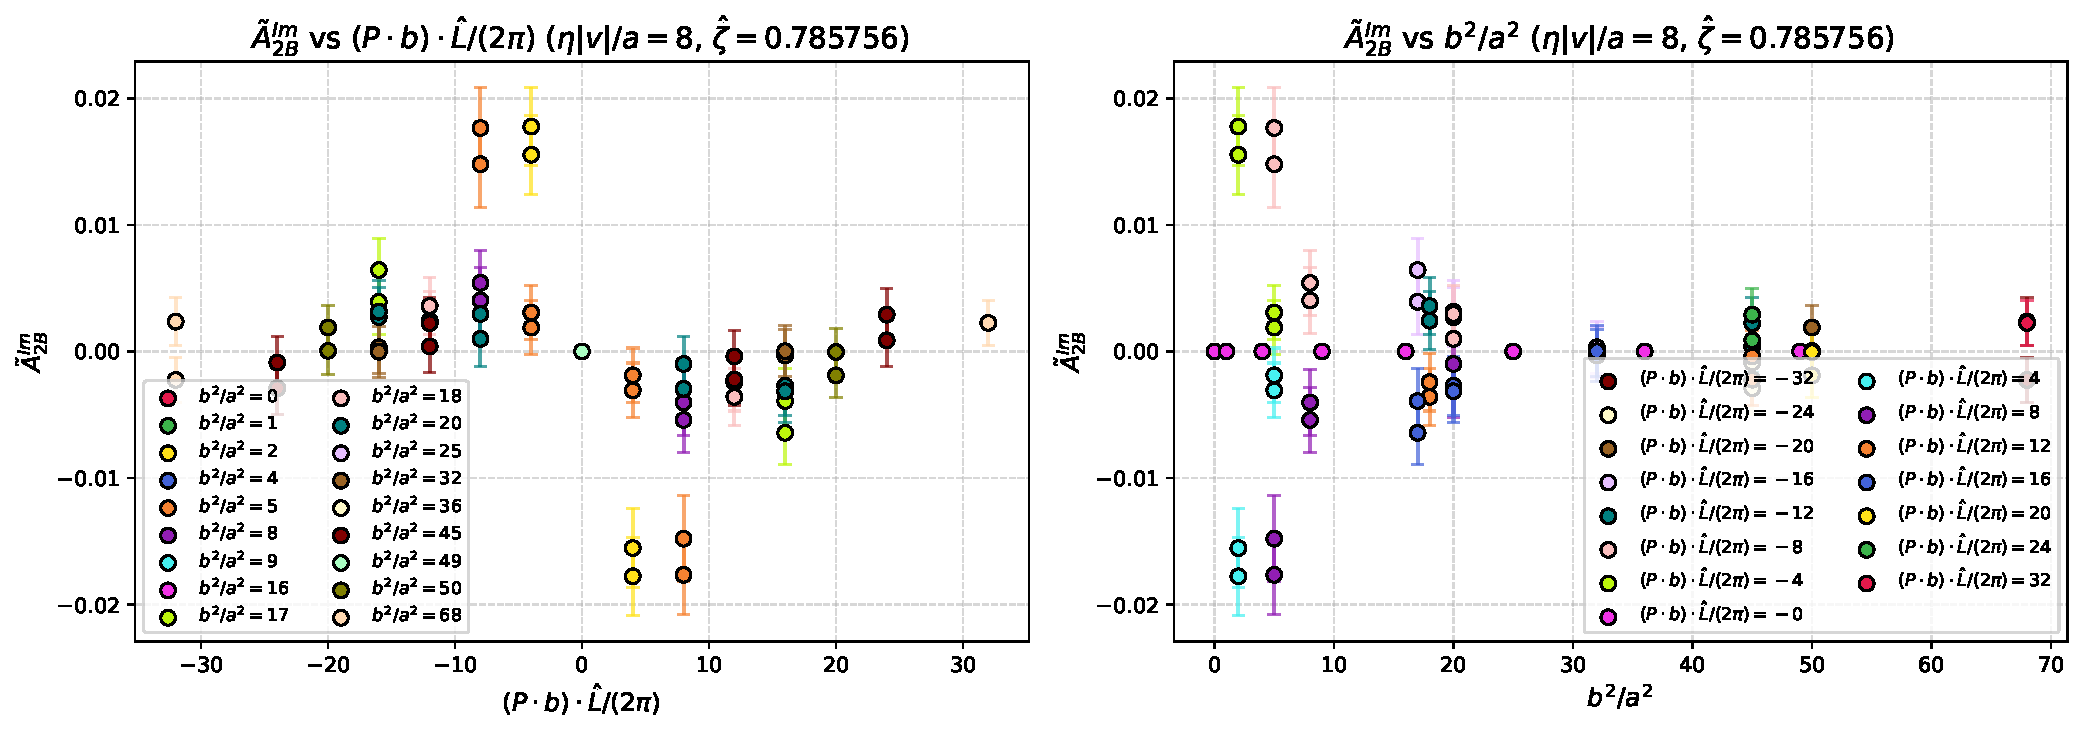
\includegraphics[width=0.98\linewidth,height=0.73\textheight,keepaspectratio]{ImA2B_Pb_bsq_eta8_PL-4_2D.pdf}\\[1mm]
{\small $\zetahat=0.785756$; $(\nu,s)$; $\eta|v|/a=8$ slices}
\figsrc{Thesis, Ch. 5: raw amplitude profiles; complete original panels.}
\end{frame}

\begin{frame}{$\tAmp_{12B}^{\mathrm{Re}}$ at $P_L=-4$: lattice coordinates}
\centering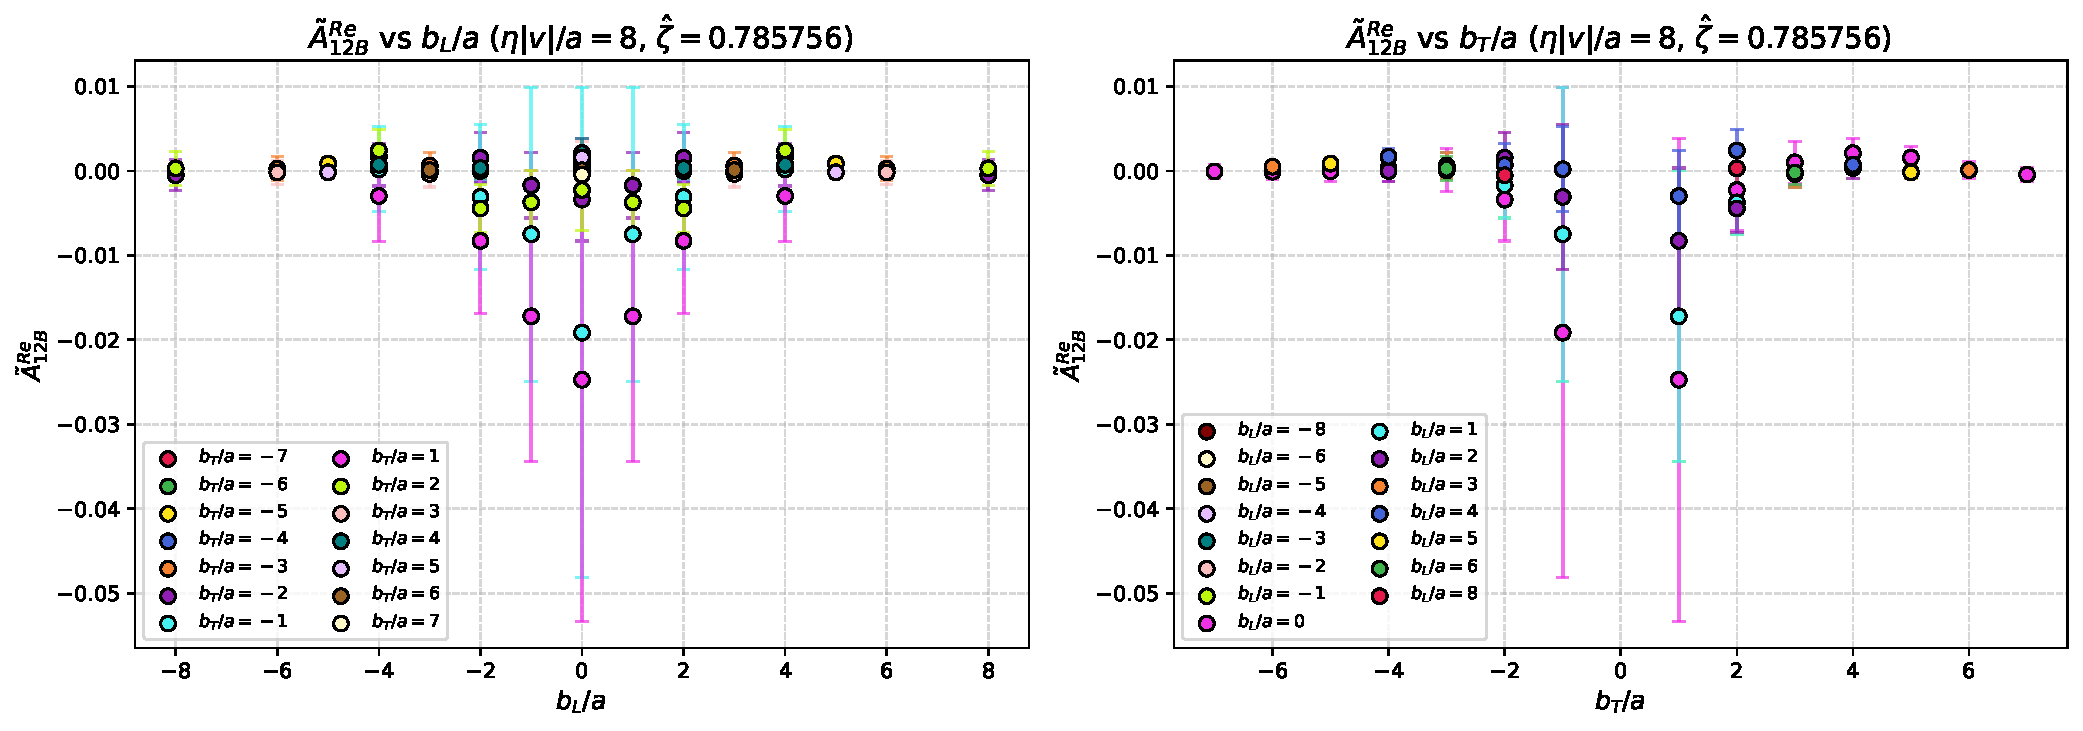
\includegraphics[width=0.98\linewidth,height=0.73\textheight,keepaspectratio]{ReA12B_eta8_PL-4_2D.pdf}\\[1mm]
{\small $\zetahat=0.785756$; $(b_L,b_T)$; $\eta|v|/a=8$ slices}
\figsrc{Thesis, Ch. 5: raw amplitude profiles; complete original panels.}
\end{frame}

\begin{frame}{$\tAmp_{12B}^{\mathrm{Re}}$ at $P_L=-4$: invariant coordinates}
\centering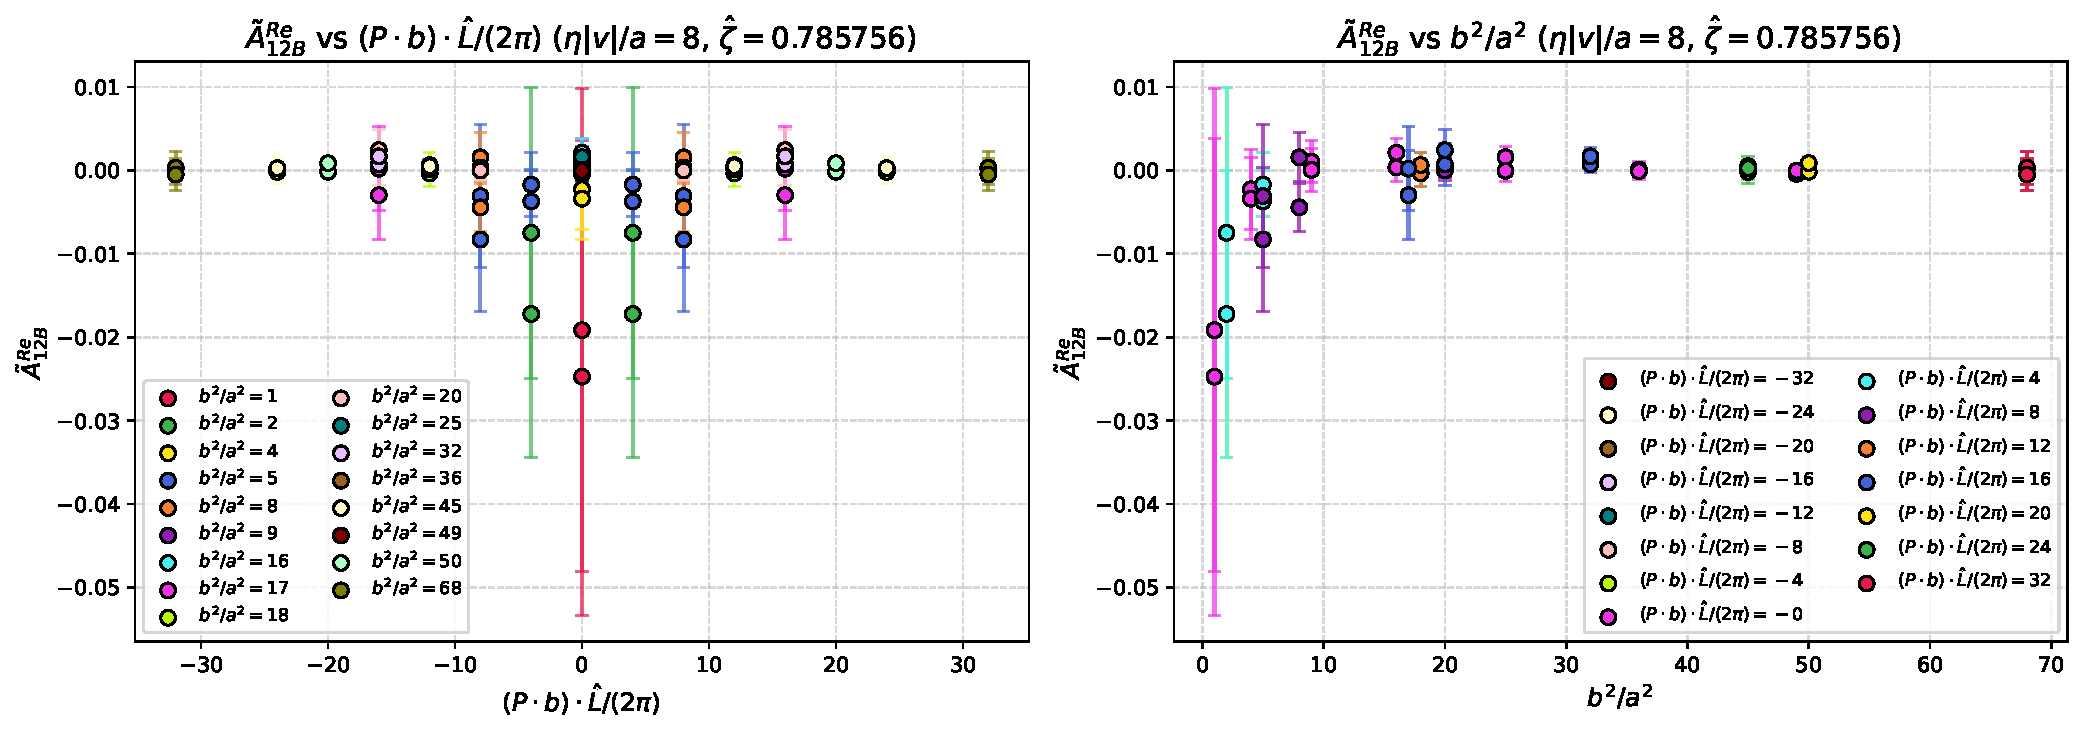
\includegraphics[width=0.98\linewidth,height=0.73\textheight,keepaspectratio]{ReA12B_Pb_bsq_eta8_PL-4_2D.pdf}\\[1mm]
{\small $\zetahat=0.785756$; $(\nu,s)$; $\eta|v|/a=8$ slices}
\figsrc{Thesis, Ch. 5: raw amplitude profiles; complete original panels.}
\end{frame}

\begin{frame}{$\tAmp_{12B}^{\mathrm{Im}}$ at $P_L=-4$: lattice coordinates}
\centering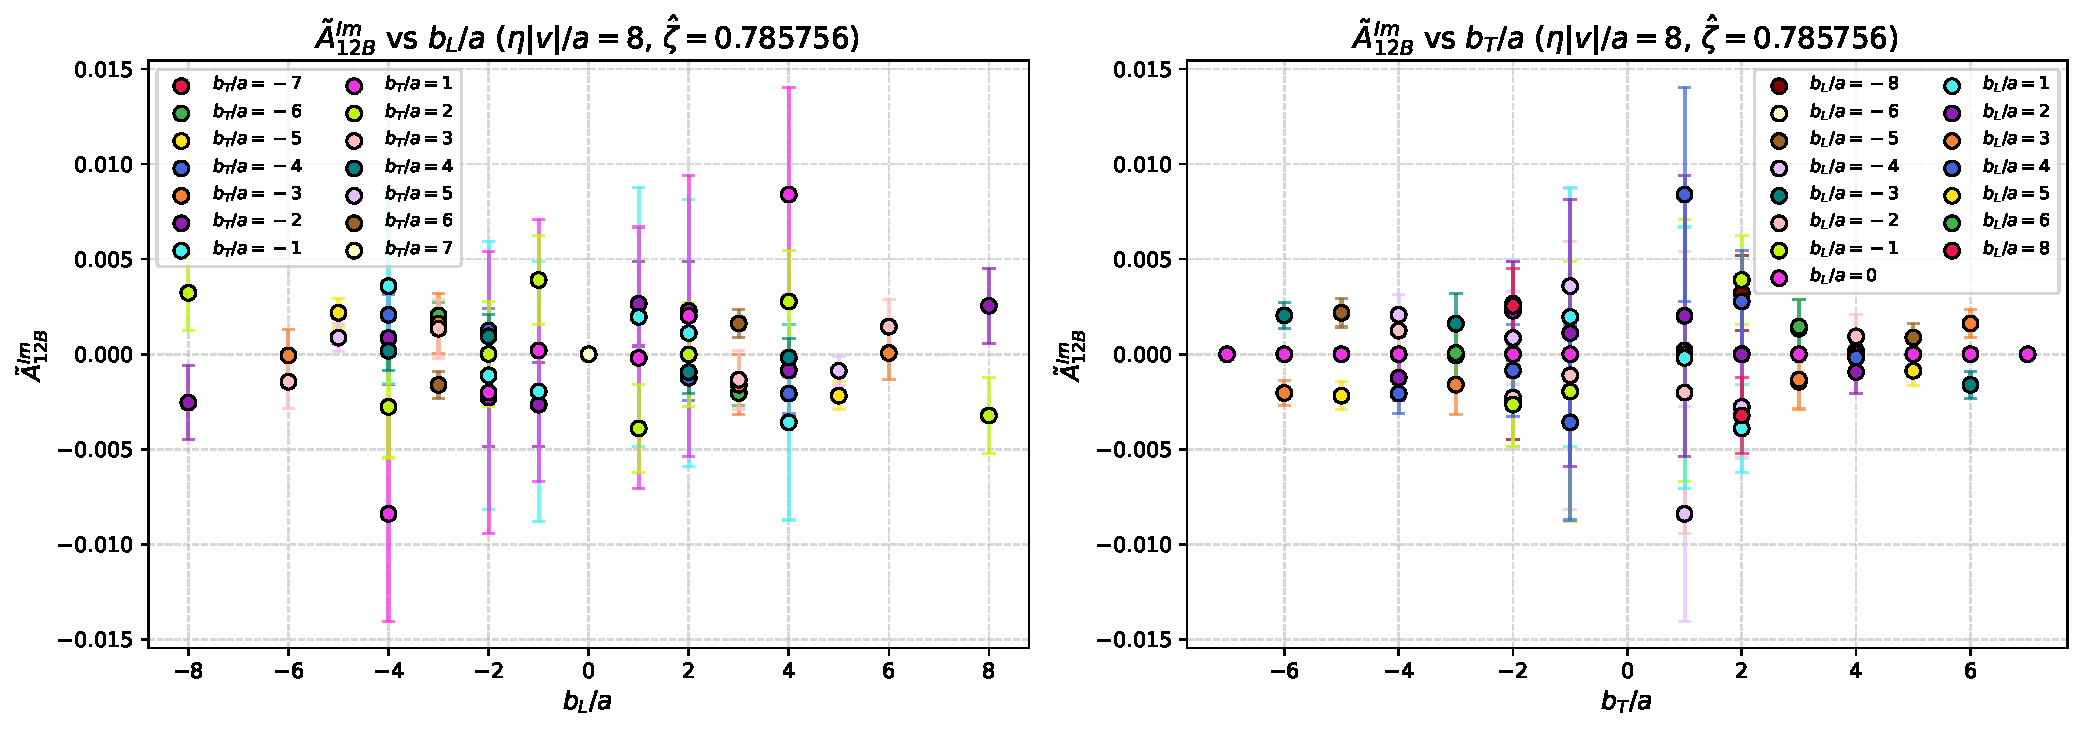
\includegraphics[width=0.98\linewidth,height=0.73\textheight,keepaspectratio]{ImA12B_eta8_PL-4_2D.pdf}\\[1mm]
{\small $\zetahat=0.785756$; $(b_L,b_T)$; $\eta|v|/a=8$ slices}
\figsrc{Thesis, Ch. 5: raw amplitude profiles; complete original panels.}
\end{frame}

\begin{frame}{$\tAmp_{12B}^{\mathrm{Im}}$ at $P_L=-4$: invariant coordinates}
\centering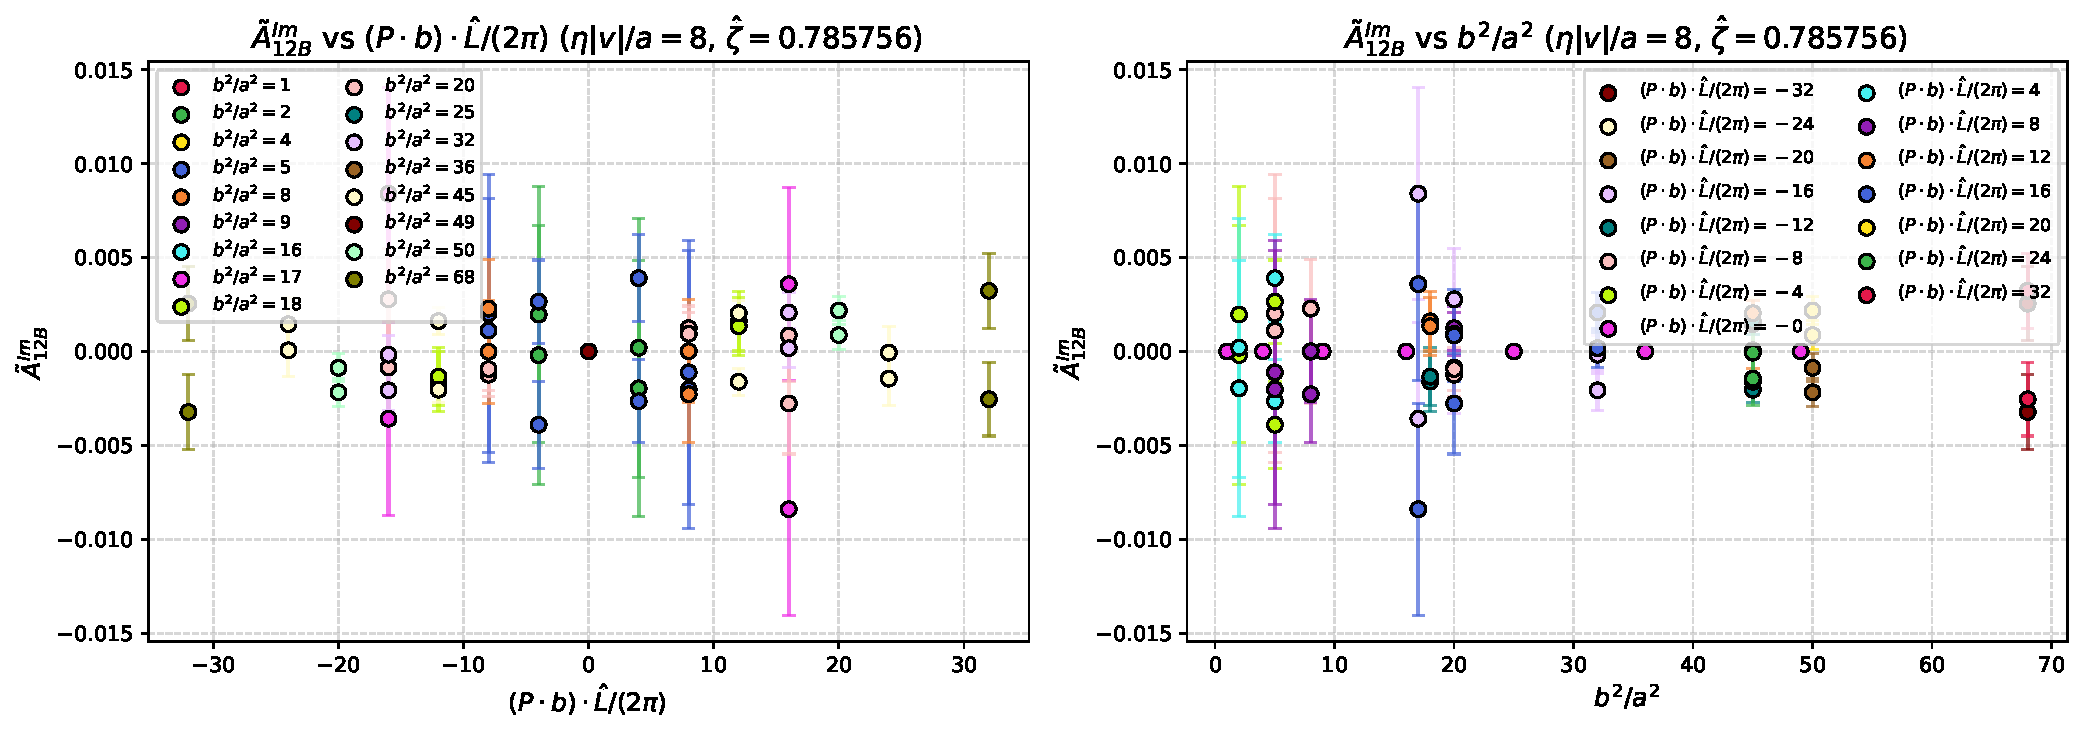
\includegraphics[width=0.98\linewidth,height=0.73\textheight,keepaspectratio]{ImA12B_Pb_bsq_eta8_PL-4_2D.pdf}\\[1mm]
{\small $\zetahat=0.785756$; $(\nu,s)$; $\eta|v|/a=8$ slices}
\figsrc{Thesis, Ch. 5: raw amplitude profiles; complete original panels.}
\end{frame}
